\documentclass[a4paper]{article}

% ========== ENCODING & LANGUAGE ==========
\usepackage{vntex}
\usepackage{mathptmx}[ptm]

% ========== MATH PACKAGES ==========
\usepackage{amsmath}
\usepackage{amsthm}
\usepackage{amssymb}
\usepackage{amscd}
\usepackage[makeroom]{cancel}

% ========== GRAPHICS & FIGURES ==========
\usepackage{graphicx}  % Replaces both graphics and epsfig
\usepackage{tikz}
\usetikzlibrary{arrows,snakes,backgrounds,calc}
\usepackage[framemethod=tikz]{mdframed}
\usepackage{color}

% ========== TABLES ==========
\usepackage{array}
\usepackage{tabularx}
\usepackage{multirow}
\usepackage{booktabs}
\usepackage{longtable}
\usepackage{diagbox}
\usepackage{hhline}

% ========== LAYOUT & FORMATTING ==========
\usepackage{geometry}
\usepackage{setspace}
\usepackage{fancyhdr}
\usepackage{lastpage}
\usepackage{float}
\usepackage{rotating}

% ========== LISTS & ENUMERATIONS ==========
\usepackage{enumerate}
\usepackage{enumitem}

% ========== TEXT FORMATTING ==========
\usepackage[normalem]{ulem}
\usepackage{alltt}

% ========== CAPTIONS ==========
\usepackage{caption}
\usepackage{subcaption}

% ========== COLUMNS ==========
\usepackage{multicol}

% ========== ALGORITHMS ==========
\usepackage[lined,boxed,commentsnumbered]{algorithm2e}

% ========== CODE LISTINGS ==========
\usepackage{listings}

% ========== HYPERLINKS (Load last) ==========
\usepackage[unicode]{hyperref}
\hypersetup{urlcolor=blue,linkcolor=black,citecolor=black,colorlinks=true}

% ========== THEOREM ENVIRONMENTS ==========
\newtheorem{theorem}{{\bf Định lý}}
\newtheorem{property}{{\bf Tính chất}}
\newtheorem{proposition}{{\bf Mệnh đề}}
\newtheorem{corollary}[proposition]{{\bf Hệ quả}}
\newtheorem{lemma}[proposition]{{\bf Bổ đề}}
\theoremstyle{definition}
\newtheorem{exer}{Bài toán}

% ========== PAGE LAYOUT ==========
% Remove page numbers from TOC, LOF, LOT
\addtocontents{toc}{\protect\thispagestyle{empty}}
\addtocontents{lof}{\protect\thispagestyle{empty}}
\addtocontents{lot}{\protect\thispagestyle{empty}}

% Geometry settings (A4: 210 × 297mm)
\def\thesislayout{	% A4: 210 × 297
	\geometry{
		a4paper,
		total={160mm,240mm},
		left=30mm,
		top=22mm,
		right=20mm,
		bottom=20mm,
	}
}
\def\thesisheadlayout{	% A4: 210 × 297
	\geometry{
		a4paper,
		total={160mm,240mm},
		left=30mm,
		top=10mm,
	}
}
\thesislayout

% ========== CODE LISTINGS SETTINGS ==========
\lstdefinelanguage{JavaScript}{
  keywords={typeof, new, true, false, catch, function, return, null, catch, switch, var, if, in, while, do, else, case, break},
  keywordstyle=\color{blue}\bfseries,
  ndkeywords={class, export, boolean, throw, implements, import, this},
  ndkeywordstyle=\color{darkgray}\bfseries,
  identifierstyle=\color{black},
  sensitive=false,
  comment=[l]{//},
  morecomment=[s]{/*}{*/},
  commentstyle=\color{purple}\ttfamily,
  stringstyle=\color{red}\ttfamily,
  morestring=[b]',
  morestring=[b]"
}

\lstset{
    language=JavaScript,
    basicstyle=\footnotesize\ttfamily,
    numbers=left,
    numberstyle=\tiny\color{gray},
    stepnumber=1,
    numbersep=5pt,
    backgroundcolor=\color{white},
    showspaces=false,
    showstringspaces=false,
    showtabs=false,
    frame=single,
    rulecolor=\color{black},
    tabsize=2,
    captionpos=b,
    breaklines=true,
    breakatwhitespace=true,
    title=\lstname,
    extendedchars=true,
    inputencoding=utf8,
    literate={á}{{\'a}}1 {à}{{\`a}}1 {ả}{{\'a}}1 {ã}{{\~a}}1 {ạ}{{\d{a}}}1
             {Á}{{\'A}}1 {À}{{\`A}}1 {Ả}{{\'A}}1 {Ã}{{\~A}}1 {Ạ}{{\d{A}}}1
             {ă}{{\u{a}}}1 {ắ}{{\'{\u{a}}}}1 {ằ}{{\`{\u{a}}}}1 {ẳ}{{\'{\u{a}}}}1 {W}{{\~{\u{a}}}}1 {ặ}{{\d{\u{a}}}}1
             {Ă}{{\u{A}}}1 {Ắ}{{\'{\u{A}}}}1 {Ằ}{{\`{\u{A}}}}1 {Ẳ}{{\'{\u{A}}}}1 {W}{{\~{\u{A}}}}1 {Ặ}{{\d{\u{A}}}}1
             {â}{{\^a}}1 {ấ}{{\'{\^a}}}1 {ầ}{{\`{\^a}}}1 {ẩ}{{\'{\^a}}}1 {ẫ}{{\~{\^a}}}1 {ậ}{{\d{\^a}}}1
             {Â}{{\^A}}1 {Ấ}{{\'{\^A}}}1 {Ầ}{{\`{\^A}}}1 {Ẩ}{{\'{\^A}}}1 {Ẫ}{{\~{\^A}}}1 {Ậ}{{\d{\^A}}}1
             {đ}{{\d{d}}}1 {Đ}{{\d{D}}}1
             {é}{{\'e}}1 {è}{{\`e}}1 {ẻ}{{\'e}}1 {ẽ}{{\~e}}1 {ẹ}{{\d{e}}}1
             {É}{{\'E}}1 {È}{{\`E}}1 {Ẻ}{{\'E}}1 {Ẽ}{{\~E}}1 {Ẹ}{{\d{E}}}1
             {ê}{{\^e}}1 {ế}{{\'{\^e}}}1 {ề}{{\`{\^e}}}1 {ể}{{\'{\^e}}}1 {ễ}{{\~{\^e}}}1 {ệ}{{\d{\^e}}}1
             {Ê}{{\^E}}1 {Ế}{{\'{\^E}}}1 {Ề}{{\`{\^E}}}1 {Ể}{{\'{\^E}}}1 {Ễ}{{\~{\^E}}}1 {Ệ}{{\d{\^E}}}1
             {í}{{\'i}}1 {ì}{{\`i}}1 {ỉ}{{\'i}}1 {ĩ}{{\~i}}1 {ị}{{\d{i}}}1
             {Í}{{\'I}}1 {Ì}{{\`I}}1 {Ỉ}{{\'I}}1 {Ĩ}{{\~I}}1 {Ị}{{\d{I}}}1
             {ó}{{\'o}}1 {ò}{{\`o}}1 {ỏ}{{\'o}}1 {õ}{{\~o}}1 {ọ}{{\d{o}}}1
             {Ó}{{\'O}}1 {Ò}{{\`O}}1 {Ỏ}{{\'O}}1 {Õ}{{\~O}}1 {Ọ}{{\d{O}}}1
             {ô}{{\^o}}1 {ố}{{\'{\^o}}}1 {ồ}{{\`{\^o}}}1 {ổ}{{\'{\^o}}}1 {ỗ}{{\~{\^o}}}1 {ộ}{{\d{\^o}}}1
             {Ô}{{\^O}}1 {Ố}{{\'{\^O}}}1 {Ồ}{{\`{\^O}}}1 {Ổ}{{\'{\^O}}}1 {Ỗ}{{\~{\^O}}}1 {Ộ}{{\d{\^O}}}1
             {ơ}{{\h{o}}}1 {ớ}{{\'{\h{o}}}}1 {ờ}{{\`{\h{o}}}}1 {ở}{{\'{\h{o}}}}1 {ỡ}{{\~{\h{o}}}}1 {ợ}{{\d{\h{o}}}}1
             {Ơ}{{\h{O}}}1 {Ớ}{{\'{\h{O}}}}1 {Ờ}{{\`{\h{O}}}}1 {Ở}{{\'{\h{O}}}}1 {Ỡ}{{\~{\h{O}}}}1 {Ợ}{{\d{\h{O}}}}1
             {ú}{{\'u}}1 {ù}{{\`u}}1 {ủ}{{\'u}}1 {ũ}{{\~u}}1 {ụ}{{\d{u}}}1
             {Ú}{{\'U}}1 {Ù}{{\`U}}1 {Ủ}{{\'U}}1 {Ũ}{{\~U}}1 {Ụ}{{\d{U}}}1
             {ư}{{\h{u}}}1 {ứ}{{\'{\h{u}}}}1 {ừ}{{\`{\h{u}}}}1 {ử}{{\'{\h{u}}}}1 {ữ}{{\~{\h{u}}}}1 {ự}{{\d{\h{u}}}}1
             {Ư}{{\h{U}}}1 {Ứ}{{\'{\h{U}}}}1 {Ừ}{{\`{\h{U}}}}1 {Ử}{{\'{\h{U}}}}1 {Ữ}{{\~{\h{U}}}}1 {Ự}{{\d{\h{U}}}}1
             {ý}{{\'y}}1 {ỳ}{{\`y}}1 {ỷ}{{\'y}}1 {ỹ}{{\~y}}1 {ỵ}{{\d{y}}}1
             {Ý}{{\'Y}}1 {Ỳ}{{\`Y}}1 {Ỷ}{{\'Y}}1 {Ỹ}{{\~Y}}1 {Ỵ}{{\d{Y}}}1
             {°}{{$^{\circ}$}}1
             {©}{{\textcopyright}}1
}
%\usepackage{fancyhdr}
\setlength{\headheight}{40pt}
\pagestyle{fancy}
\fancyhead{} % clear all header fields
\renewcommand{\footruleskip}{1mm}

\fancyhead[L]{
 \begin{tabular}{rl}
    \begin{picture}(25,15)(0,0)
    \put(0,-8){
\includegraphics[width=10mm, height=10mm]{Images/hcmut.png}}
    %\put(0,-8){
\epsfig{width=10mm,figure=hcmut.eps}}
   \end{picture}&
	%
\includegraphics[width=8mm, height=8mm]{hcmut.png} & %
	\begin{tabular}{l}
		\textbf{  Trường Đại Học Bách Khoa - Đại học Quốc gia TP.HCM }\\
		\textbf{  Khoa Khoa Học \& Kỹ Thuật Máy Tính}
	\end{tabular} 	
 \end{tabular}
}
\fancyhead[R]{
	\begin{tabular}{l}
		\tiny \bf \\
		\tiny \bf 
	\end{tabular}  }
\fancyfoot{} % clear all footer fields
\fancyfoot[L]{\scriptsize  Báo cáo Đồ án kỹ thuật máy tính (CO4041) - HK1 2025 - 2026}
\fancyfoot[R]{\scriptsize  Trang {\thepage}/\pageref{LastPage}}

\renewcommand{\headrulewidth}{0.3pt}
\renewcommand{\footrulewidth}{0.3pt}

%%%
\setcounter{secnumdepth}{4}
\setcounter{tocdepth}{3}
% ========== SECTION NUMBERING (4 levels) ==========
\makeatletter
\newcounter{subsubsubsection}[subsubsection]
\renewcommand\thesubsubsubsection{\thesubsubsection .\@alph\c@subsubsubsection}
\newcommand\subsubsubsection{\@startsection{subsubsubsection}{4}{\z@}%
    {-3.25ex\@plus -1ex \@minus -.2ex}%
    {1.5ex \@plus .2ex}%
    {\normalfont\normalsize\bfseries}}
\newcommand*\l@subsubsubsection{\@dottedtocline{3}{10.0em}{4.1em}}
\newcommand*{\subsubsubsectionmark}[1]{}
\makeatother

% ========== MATH & CAPTION FORMATTING ==========
\everymath{\color{black}}
\sloppy

% Caption settings
\captionsetup[figure]{
    labelfont={small,bf},
    textfont={small,it},
    belowskip=-1pt,
    aboveskip=-9pt
}
\captionsetup[table]{
    labelfont={small,bf},
    textfont={small,it},
    belowskip=-1pt,
    aboveskip=7pt
}

% Float spacing
\setlength{\floatsep}{5pt plus 2pt minus 2pt}
\setlength{\textfloatsep}{5pt plus 2pt minus 2pt}
\setlength{\intextsep}{10pt plus 2pt minus 2pt}

\thesislayout

% ========== BEGIN DOCUMENT ==========

\begin{document}

\begin{titlepage}
\thispagestyle{empty}
\begin{tikzpicture}[remember picture, overlay]
  \draw[line width = 4pt] ($(current page.north west) + (1cm,-1cm)$) rectangle ($(current page.south east) + (-1cm,1cm)$);
  \draw[line width=1.5pt]
    ($ (current page.north west) + (1.1cm,-1.1cm) $)
    rectangle
    ($ (current page.south east) + (-1.1cm,1.1cm) $);
\end{tikzpicture}

\begin{center}
\LARGE \textbf{ĐẠI HỌC QUỐC GIA THÀNH PHỐ HỒ CHÍ MINH} \\
\vspace{0.2cm}
\LARGE \textbf{TRƯỜNG ĐẠI HỌC BÁCH KHOA} \\
\vspace{0.2cm}
\LARGE \textbf{KHOA KHOA HỌC VÀ KĨ THUẬT MÁY TÍNH}
\end{center}

\vspace{0.3cm}

\begin{figure}[h!]
\begin{center}

\includegraphics[width=4cm]{Images/hcmut.png}
\end{center}
\end{figure}

\begin{center}
\begin{tabular}{c}
\multicolumn{1}{c}{\textbf{{\LARGE BÁO CÁO}}}\\
% \\{\textbf{{\LARGE ĐỒ ÁN CHUYÊN NGÀNH}}}
\\{\textbf{{\LARGE ĐỒ ÁN KỸ THUẬT MÁY TÍNH}}}

% \\ \textit{(SV chọn tên môn học cho phù hợp)}
\\
\\
\textbf{\LARGE Xây dựng thuật toán tính toán tọa độ mục tiêu từ dữ liệu GPS }\\
\textbf{\LARGE  góc ngắm và khoảng cách}
\\ \textit{}

\\ \vspace{0.5cm} {\Large NGÀNH: Kĩ Thuật Máy Tính}
\end{tabular}
\end{center}
\vspace{0.5cm}
\begin{center}
    


\begin{tabular}{lll}
\hspace{6 cm} &  \textbf{\Large HỘI ĐỒNG:} {\Large ................................}
\\
\\
\hspace{6 cm} &   \textbf{\Large GVHD:} {\Large TS VÕ TUẤN BÌNH}
\\
\\
\hspace{6 cm}  &   \textbf{\Large TKHĐ:} {\Large ................................}
\\
\\
% TKHĐ là THƯ KÝ HỘI ĐỒNG
\hspace{6 cm} &     \textbf{$\;$ $\;$$\;$$\;$$\;$$\;$$\;$$\;$$\;$$\;$$\;$$\;$$\;$$\;$$\;$$\;$$\;$$\;$$\;$$\;$$\;$$\;$$\;$$\;$$\;$$\;$$\;$$\;$$\;$$\;$$\;$$\;$$\;$$\;$ \Large ---o0o---} 
\\
\\
\hspace{6 cm} &   \textbf{\Large SVTH1:} {\Large Huỳnh Gia Qui (2112138)}
\\
\\
\hspace{6 cm}&   \textbf{\Large SVTH2:}  {\Large Bùi Nguyễn Thành Luân (2111700)}
\\
\\
\hspace{6 cm} &   \textbf{\Large SVTH3:}  {\Large Nguyễn Trung Hiếu (2113357 )}
\\
\\
\end{tabular}

\end{center}
\vspace{0.5cm}
\begin{center}
{\Large TP. HỒ CHÍ MINH, 01/2026 }
\end{center}
\end{titlepage}
%\thispagestyle{empty}
\newpage
%%%%%%%%%%%%%%%%%INTRO%%%%%%%%%%%%%%%%%%%
\section*{Lời cảm ơn}
\thispagestyle{empty}

\addcontentsline{toc}{section}{Lời cảm ơn}

Trong quá trình thực hiện đồ án “\textit{Xây dựng thuật toán tính toán tọa độ mục tiêu từ dữ liệu GPS, góc ngắm và khoảng cách}”, nhóm chúng em đã nhận được nhiều sự giúp đỡ quý báu từ các thầy cô, gia đình và bạn bè. Chúng em xin chân thành bày tỏ lòng biết ơn sâu sắc đến những người đã góp phần vào sự hoàn thành của đồ án này.

Trước hết, nhóm xin gửi lời cảm ơn sâu sắc tới \textbf{Thầy Võ Tuấn Bình} — người hướng dẫn chính đã tận tình chỉ bảo, góp ý quý giá và tạo điều kiện thuận lợi cho nhóm trong suốt quá trình thực hiện đề tài. Những gợi ý chuyên môn và sự hỗ trợ của thầy là nền tảng quan trọng giúp nhóm hoàn thiện báo cáo này.

Chúng em cũng xin cảm ơn \textbf{Khoa Khoa học và Kỹ thuật Máy tính, Trường Đại học Bách Khoa TP.HCM} đã cung cấp môi trường học tập, tài liệu và cơ sở vật chất cần thiết. Xin cảm ơn các thầy cô trong khoa đã giảng dạy và truyền đạt kiến thức quý báu.

Đặc biệt, nhóm xin cảm ơn gia đình và bạn bè đã luôn động viên, hỗ trợ về mặt tinh thần và vật chất để nhóm có thể hoàn thành đồ án. Những góp ý, trao đổi ý tưởng và sự giúp đỡ kịp thời của các bạn đã giúp nhóm khắc phục nhiều khó khăn trong quá trình thực hiện.

Mặc dù đã cố gắng hoàn thành tốt nhất, đồ án còn tồn tại những hạn chế. Nhóm rất mong nhận được ý kiến đóng góp từ quý thầy cô và bạn đọc để đồ án được hoàn thiện hơn.


\clearpage
\pagenumbering{arabic}

% \input{Intro/LoiCamDoan}
% \section*{Nội dung báo cáo tuần}
\thispagestyle{empty}

\subsection*{Tuần 1}
\begin{itemize}
    \item Nghiên cứu tổng quan về bài toán cần giải quyết
    \item Khái niệm về GPS và nguyên lí hoạt động cũng như cách tính toán
\end{itemize}
\subsection*{Tuần 2}
\begin{itemize}
    \item Hệ thống lại các hệ tọa độ cũng như cách chuyển đổi giữa chúng
    \item Tam giác cầu, mỗi quan hệ với vecto định hướng 3D
    \item Các phép chiếu bản đồ phổ biến
\end{itemize}

\subsection*{Tuần 3}

\begin{itemize}
    \item Chuyển đổi góc azimuth và elevation thành vector định hướng 3D
    \item Tính toán tọa độ mục tiêu 3D từ vector định hướng và khoảng cách laser
\end{itemize}

\subsection*{Mục tiêu tuần 4}
\begin{itemize}
    \item Xử lý dữ liệu cảm biến GPS, IMU và Laser: Hiệu chuẩn, Fusion và Lọc nhiễu
\end{itemize}

\clearpage
\pagenumbering{arabic}

\newpage
\tableofcontents
\newpage
\listoffigures
\newpage
\listoftables
\newpage
\setcounter{page}{1}

%%%%%%%%%%%%%%%%%CONTENTS%%%%%%%%%%%%%%%%%%%
\section{Giới thiệu}
\begin{itemize}
    \item Trong các hệ thống chỉ huy - điều khiển hỏa lực, việc tính toán chính xác vị trí mục tiêu dựa trên thông tin đo thực địa là yếu tố quyết định thành công. Đồ án này nhằm xây dựng thuật toán xác định tọa độ địa lý (kinh độ, vĩ độ, cao độ) của mục tiêu từ các dữ liệu: vị trí GPS của người quan sát, góc ngắm (azimuth, elevation) đo từ IMU/la bàn, khoảng cách trực tiếp đo bằng laser rangefinder. Dữ liệu này sẽ được chuyển đổi thành nhiều hệ tọa độ trung gian (ECEF, ENU/NED) để thuận tiện cho xử lý số, góp phần hiển thị tọa độ mục tiêu trên bản đồ số (WebGIS), phục vụ nhiều ứng dụng quân sự và dân sự. 
    \item Việc xác định tọa độ mục tiêu trong không gian thực dựa trên thông tin vị trí GPS, góc ngắm (azimuth, elevation) và khoảng cách đo bằng laser là bài toán nền tảng trong lĩnh vực quân sự (chỉ huy hỏa lực, định vị mục tiêu), GIS thực địa, robotics và tự động hóa di động. Hệ thống này có vai trò “giao tiếp” giữa thế giới thực (tọa độ địa lý) và bài toán động học, phục vụ cả việc tác chiến chính xác, khảo sát bản đồ cũng như định vị đối tượng di động hoặc cố định trong môi trường không đồng nhất.
    \item Yêu cầu của đồ án hướng đến việc thu thập, tổng hợp, xử lý các thông tin từ tổ hợp đa cảm biến (GPS, cảm biến đo khoảng cách laser LiDAR hoặc Time-of-Flight, la bàn điện tử...), tính toán kết hợp cả góc ngắm không gian (phổ biến là azimuth/elevation), đồng thời giải bài toán chuyển đổi qua lại giữa các hệ tọa độ bản đồ thực tế (WGS84, VN2000, UTM v.v...).

\end{itemize}



\newpage
\section{Tổng quan Nghiên cứu Liên quan}

Phần này trình bày tổng quan về các nghiên cứu, hệ thống và phương pháp liên quan đến tính toán tọa độ mục tiêu từ dữ liệu GPS, góc phương vị và khoảng cách. Việc nghiên cứu các công trình trước đây giúp định vị đúng vị trí của đề tài, xác định khoảng trống nghiên cứu và đưa ra định hướng phát triển phù hợp.

\subsection{Lịch sử Phát triển Hệ thống Định vị}

\subsubsection{Từ Định vị Truyền thống đến GPS}
Trước khi GPS ra đời, các phương pháp định vị chủ yếu dựa vào:
\begin{itemize}
    \item \textbf{Thiên văn định vị}: Sử dụng quan sát các thiên thể (mặt trời, sao) để xác định vị trí. Phương pháp này được hàng hải sử dụng từ thế kỷ 15, có độ chính xác khoảng 1-2 hải lý ($\sim$2-4 km) \cite{hofmann2012global}.
    
    \item \textbf{Tam giác đạc}: Đo góc và khoảng cách đến các điểm mốc đã biết. Được Charles Mason và Jeremiah Dixon sử dụng để đo đạc biên giới Maryland-Pennsylvania (1763-1767), độ chính xác $\sim$10m với khoảng cách ngắn.
    
    \item \textbf{Radio navigation}: LORAN (Long Range Navigation) phát triển trong Thế chiến II, sử dụng sự chênh lệch thời gian tín hiệu radio từ nhiều trạm phát. Độ chính xác $\sim$200m-2km tùy khoảng cách \cite{kaplan2017understanding}.
\end{itemize}

GPS (Global Positioning System) được Bộ Quốc phòng Mỹ phát triển từ thập niên 1970, hoạt động chính thức năm 1995 với 24 vệ tinh. Đây là bước nhảy vọt về độ chính xác (từ km xuống m) và khả năng phủ sóng toàn cầu 24/7.

\subsubsection{Các Hệ thống GNSS Toàn cầu}
Hiện nay có 4 hệ thống định vị vệ tinh toàn cầu (GNSS):

\begin{table}[H]
\centering
\begin{tabular}{|l|c|c|c|p{4cm}|}
\hline
\textbf{Hệ thống} & \textbf{Quốc gia} & \textbf{Số vệ tinh} & \textbf{Độ chính xác} & \textbf{Ghi chú} \\
\hline
GPS & Mỹ & 31 & 5-10m & Hoạt động từ 1995 \\
\hline
GLONASS & Nga & 24 & 5-10m & Phục hồi đầy đủ 2011 \\
\hline
Galileo & EU & 30 & 1m (dân sự) & Hoạt động từ 2016 \\
\hline
BeiDou & Trung Quốc & 35 & 10m (toàn cầu) & Hoàn thành 2020 \\
\hline
\end{tabular}
\caption{So sánh các hệ thống GNSS toàn cầu \cite{groves2013principles}}
\end{table}

Việc kết hợp nhiều hệ thống GNSS (multi-GNSS) giúp:
\begin{itemize}
    \item Tăng số lượng vệ tinh khả dụng (từ 8-12 lên 20-30)
    \item Cải thiện độ chính xác (geometric dilution of precision - GDOP tốt hơn)
    \item Tăng độ tin cậy trong môi trường đô thị (urban canyon)
\end{itemize}

\subsection{Các Phương pháp Tính toán Geodesic}

\subsubsection{Mô hình Cầu và Haversine Formula}
Công thức Haversine được R.W. Sinnott công bố năm 1984 \cite{sinnot1984virtues}, dựa trên giả định Trái Đất là hình cầu hoàn hảo với bán kính R = 6371 km. Công thức này đơn giản nhưng hiệu quả cho khoảng cách ngắn:

\begin{equation}
\begin{aligned}
a &= \sin^2\left(\frac{\Delta\varphi}{2}\right) + \cos\varphi_1 \cdot \cos\varphi_2 \cdot \sin^2\left(\frac{\Delta\lambda}{2}\right) \\
c &= 2 \cdot \arctan2\left(\sqrt{a}, \sqrt{1-a}\right) \\
d &= R \cdot c
\end{aligned}
\end{equation}

\textbf{Ưu điểm}:
\begin{itemize}
    \item Tính toán nhanh ($\sim$0.002ms)
    \item Code đơn giản, dễ implement
    \item Độ chính xác chấp nhận được (<0.5\% với d<100km)
\end{itemize}

\textbf{Nhược điểm}:
\begin{itemize}
    \item Sai số tăng nhanh với khoảng cách lớn
    \item Không chính xác ở vĩ độ cao (>60°)
    \item Bỏ qua hình dạng ellipsoid thực của Trái Đất
\end{itemize}

\subsubsection{Vincenty Formula và Ellipsoid WGS-84}
Thaddeus Vincenty (1975) phát triển công thức chính xác trên ellipsoid WGS-84 \cite{vincenty1975direct}, sử dụng phương pháp lặp (iterative) để tìm geodesic (đường ngắn nhất trên ellipsoid).

Công thức Vincenty direct problem (tìm điểm đích từ điểm xuất phát, azimuth và khoảng cách):

\begin{equation}
\begin{aligned}
\tan U_1 &= (1-f) \tan\varphi_1 \\
\sigma_1 &= \arctan2(\tan U_1, \cos\alpha_1) \\
\sin\alpha &= \cos U_1 \sin\alpha_1 \\
\cos^2\alpha &= 1 - \sin^2\alpha \\
u^2 &= \cos^2\alpha \frac{a^2 - b^2}{b^2}
\end{aligned}
\end{equation}

Sau đó lặp để tìm $\sigma$ (angular distance), và cuối cùng tính $\varphi_2, \lambda_2$.

\textbf{Ưu điểm}:
\begin{itemize}
    \item Độ chính xác cực cao ($\sim$0.1mm trên 1000km)
    \item Stable với hầu hết các trường hợp
    \item Chuẩn được sử dụng trong surveying/geodesy
\end{itemize}

\textbf{Nhược điểm}:
\begin{itemize}
    \item Phức tạp hơn $\sim$10x so với Haversine
    \item Chậm hơn $\sim$10x ($\sim$0.02ms)
    \item Có thể không converge gần antipodal points
\end{itemize}

\subsubsection{Karney Algorithm}
Charles Karney (2013) cải tiến Vincenty với thuật toán ổn định hơn \cite{karney2013algorithms}, giải quyết được vấn đề convergence và cung cấp độ chính xác $\sim$15 nanometers.

\textbf{So sánh các thuật toán}:
\begin{table}[H]
\centering
\small
\begin{tabular}{|l|c|c|c|c|}
\hline
\textbf{Thuật toán} & \textbf{Độ chính xác} & \textbf{Tốc độ} & \textbf{Độ phức tạp} & \textbf{Stability} \\
\hline
Haversine & 0.5\% -> 100km & Nhanh & Thấp & Tốt \\
\hline
Vincenty & 0.1mm -> 1000km & Trung bình & Cao & Khá tốt \\
\hline
Karney & 15nm -> global & Trung bình & Cao & Rất tốt \\
\hline
\end{tabular}
\caption{So sánh các thuật toán tính geodesic}
\end{table}

\subsection{Nghiên cứu về Sensor Fusion}

\subsubsection{Kalman Filter trong GPS/INS Integration}
Kalman Filter (1960) là nền tảng của sensor fusion hiện đại. Extended Kalman Filter (EKF) được ứng dụng rộng rãi trong tích hợp GPS và IMU (Inertial Measurement Unit) \cite{groves2013principles}.

\textbf{Ý tưởng cốt lõi}:
\begin{itemize}
    \item GPS: Độ chính xác cao nhưng tần số thấp (1-10 Hz), có thể bị mất tín hiệu
    \item IMU: Tần số cao (100-1000 Hz), nhưng drift theo thời gian
    \item Kết hợp: Lấy ưu điểm của cả hai, giảm nhược điểm
\end{itemize}

Mô hình toán học EKF cho GPS/IMU:
\begin{equation}
\begin{aligned}
\mathbf{x}_{k|k-1} &= f(\mathbf{x}_{k-1}, \mathbf{u}_k) \quad \text{(Prediction)} \\
\mathbf{P}_{k|k-1} &= \mathbf{F}_k \mathbf{P}_{k-1} \mathbf{F}_k^T + \mathbf{Q}_k \\
\mathbf{K}_k &= \mathbf{P}_{k|k-1} \mathbf{H}_k^T (\mathbf{H}_k \mathbf{P}_{k|k-1} \mathbf{H}_k^T + \mathbf{R}_k)^{-1} \\
\mathbf{x}_k &= \mathbf{x}_{k|k-1} + \mathbf{K}_k(\mathbf{z}_k - h(\mathbf{x}_{k|k-1})) \quad \text{(Update)}
\end{aligned}
\end{equation}

Trong đó:
\begin{itemize}
    \item $\mathbf{x}$: State vector (position, velocity, orientation, IMU biases)
    \item $\mathbf{P}$: Covariance matrix
    \item $\mathbf{K}$: Kalman gain
    \item $\mathbf{Q}$: Process noise covariance
    \item $\mathbf{R}$: Measurement noise covariance
\end{itemize}

\subsubsection{Adaptive Filtering}
Trong môi trường động (GPS intermittent, varying noise), Adaptive Kalman Filter tự động điều chỉnh $\mathbf{Q}$ và $\mathbf{R}$ dựa trên innovation sequence \cite{simon2006optimal}:

\begin{equation}
\begin{aligned}
\mathbf{r}_k &= \mathbf{z}_k - h(\mathbf{x}_{k|k-1}) \quad \text{(Innovation)} \\
\mathbf{C}_r &= \frac{1}{N}\sum_{i=k-N+1}^{k} \mathbf{r}_i \mathbf{r}_i^T \quad \text{(Sample covariance)} \\
\hat{\mathbf{R}}_k &= \mathbf{C}_r - \mathbf{H}_k \mathbf{P}_{k|k-1} \mathbf{H}_k^T \quad \text{(Adaptive R)}
\end{aligned}
\end{equation}

\subsection{Hệ thống Web-based GIS và Mapping}

\subsubsection{Web Mapping Libraries}
Các thư viện web mapping phổ biến:

\begin{enumerate}
    \item \textbf{Leaflet.js} \cite{leafletjs}:
    \begin{itemize}
        \item Open-source, lightweight ($\sim$42KB)
        \item Mobile-friendly
        \item Plugin ecosystem phong phú
        \item Sử dụng: OpenStreetMap, MapBox, custom tiles
    \end{itemize}
    
    \item \textbf{OpenLayers}:
    \begin{itemize}
        \item More features ($\sim$250KB), phức tạp hơn
        \item Hỗ trợ nhiều projections (EPSG codes)
        \item Vector tiles, 3D capabilities
    \end{itemize}
    
    \item \textbf{Mapbox GL JS}:
    \begin{itemize}
        \item GPU-accelerated rendering
        \item Beautiful styling, smooth interactions
        \item Commercial (cần API key)
    \end{itemize}
    
    \item \textbf{Google Maps API}:
    \begin{itemize}
        \item Comprehensive features
        \item Best data coverage
        \item Expensive ($7/1000$ loads)
    \end{itemize}
\end{enumerate}

\textbf{Lựa chọn Leaflet cho dự án}:
\begin{itemize}
    \item Open-source, không giới hạn
    \item Đủ nhẹ cho prototype/MVP
    \item Community support tốt
    \item Dễ offline (với MBTiles)
\end{itemize}

\subsubsection{Map Projections và Web Mercator}
Hầu hết web maps sử dụng Web Mercator (EPSG:3857), một biến thể của Mercator projection \cite{snyder1987map}:

\begin{equation}
\begin{aligned}
x &= R \cdot \lambda \\
y &= R \cdot \ln\left[\tan\left(\frac{\pi}{4} + \frac{\varphi}{2}\right)\right]
\end{aligned}
\end{equation}

\textbf{Ưu điểm}:
\begin{itemize}
    \item Conformal (bảo toàn góc, hình dạng local)
    \item Rhumb lines (constant bearing) là đường thẳng
    \item Tiles dễ cache (256×256 pixels)
\end{itemize}

\textbf{Nhược điểm}:
\begin{itemize}
    \item Biến dạng diện tích lớn (Greenland $\sim$ Africa)
    \item Không dùng được cho vĩ độ >85°
    \item Không phải geodesic (đường ngắn nhất bị cong)
\end{itemize}

\subsection{Ứng dụng Thực tế}

\subsubsection{Military Applications}
\begin{itemize}
    \item \textbf{Artillery Targeting Systems}: Hệ thống như AFATDS (Advanced Field Artillery Tactical Data System) sử dụng GPS+IMU+laser rangefinder để tính toán fire missions \cite{kaplan2017understanding}.
    
    \item \textbf{Forward Observer Tools}: ATAK (Android Tactical Assault Kit) - Android app cho soldiers, tính toán target coordinates từ observer position + bearing + distance.
    
    \item \textbf{Precision-Guided Munitions}: GPS-guided bombs (JDAM) có độ chính xác $\sim$5m CEP (Circular Error Probable).
\end{itemize}

\subsubsection{Search and Rescue}
\begin{itemize}
    \item SAR teams sử dụng handheld GPS + compass + visual range estimation
    \item RECCO system: Reflector-based location (không cần battery)
    \item Drone-assisted SAR: Tích hợp gimbal angles để tính victim location
\end{itemize}

\subsubsection{Surveying and Construction}
\begin{itemize}
    \item Total Stations: Tích hợp theodolite + EDM (Electronic Distance Measurement), độ chính xác $\sim$1mm -> 1km
    \item RTK GPS: Real-Time Kinematic, cm-level accuracy
    \item BIM (Building Information Modeling): Tích hợp GPS data vào 3D models
\end{itemize}

\subsection{Khoảng trống Nghiên cứu}

Từ tổng quan nghiên cứu, nhận thấy:

\begin{enumerate}
    \item \textbf{Thiếu hệ thống lightweight}: Các giải pháp thương mại (ATAK, AFATDS) phức tạp, đắt tiền. Cần giải pháp đơn giản, open-source cho education/training.
    
    \item \textbf{Thiếu phân tích sai số tổng hợp}: Hầu hết nghiên cứu tập trung vào GPS error hoặc IMU error riêng lẻ, ít phân tích error propagation toàn hệ thống.
    
    \item \textbf{Web-based gap}: Các công cụ hiện có chủ yếu là desktop/mobile apps, ít giải pháp web-based dễ triển khai.
    
    \item \textbf{Thiếu so sánh Haversine vs Vincenty}: Ít nghiên cứu định lượng trade-off accuracy vs. performance cho use cases khác nhau.
\end{enumerate}

Dự án này đóng góp vào các khoảng trống trên bằng cách:
\begin{itemize}
    \item Xây dựng hệ thống open-source, web-based, lightweight
    \item Phân tích chi tiết error propagation từ sensors đến output
    \item So sánh định lượng Haversine vs. Vincenty
    \item Cung cấp educational tool với visualization trực quan
\end{itemize}

\newpage
\section{Cơ sở lý thuyết}
\subsection{Hệ thống Định vị Toàn cầu GPS}
\subsubsection{GPS là gì}
GPS là hệ thống định vị toàn cầu dựa trên mạng lưới các vệ tinh nhân tạo quay quanh Trái Đất. Hệ thống này được thiết kế, xây dựng và vận hành bởi Bộ Quốc phòng Hoa Kỳ, ban đầu phục vụ mục đích quân sự, sau đó mở rộng cho dân sự từ thập niên 1980.

\subsubsection{Cấu trúc hệ thống}
GPS gồm ba thành phần chính:
\begin{itemize}
    \item Phần không gian (Space Segment): gồm 30 vệ tinh (27 vệ tinh hoạt động và 3 vệ tinh dự phòng) nằm trên các quỹ đạo xoay quanh Trái Đất. Chúng cách mặt đất 20.200 km, bán kính quỹ đạo 26.600 km. Chúng chuyển động ổn định và quay hai vòng quỹ đạo trong khoảng thời gian gần 24 giờ với vận tốc 7 nghìn dặm một giờ. Các vệ tinh trên quỹ đạo được bố trí sao cho các máy thu GPS trên mặt đất có thể nhìn thấy tối thiểu 4 vệ tinh vào bất kỳ thời điểm nào.
    \item Phần điều khiển (Control Segment): kiểm soát vệ tinh đi đúng hướng theo quỹ đạo và thông tin thời gian chính xác. Có 5 trạm kiểm soát đặt rải rác trên Trái Đất. Bốn trạm kiểm soát hoạt động một cách tự động, và một trạm kiểm soát là trung tâm. Bốn trạm này nhận tín hiệu liên tục từ những vệ tinh và gửi các thông tin này đến trạm kiểm soát trung tâm. Tại trạm kiểm soát trung tâm, nó sẽ sửa lại dữ liệu cho đúng và kết hợp với hai an-ten khác để gửi lại thông tin cho các vệ tinh. Ngoài ra, còn một trạm kiểm soát trung tâm dự phòng và sáu trạm quan sát chuyên biệt.
    \item Phần người dùng (User Segment): các thiết bị thu GPS (điện thoại, ô tô, tàu thuyền, máy bay…).
\end{itemize}

\subsubsection{Nguyên lý hoạt động}
\begin{itemize}
    \item Mỗi vệ tinh GPS phát tín hiệu chứa thời gian phát và vị trí chính xác $(x_i,y_i,z_i)$ của vệ tinh tại thời điểm đó. 
    \item Thiết bị thu GPS nhận tín hiệu và so sánh thời gian phát với thời gian nhận → tính được khoảng cách đến vệ tinh $R_i$.
    \item Để xác định vị trí trong không gian 3D, cần ít nhất 4 vệ tinh:
    \begin{itemize}
        \item 3 vệ tinh để tính vĩ độ, kinh độ, độ cao.
        \item 1 vệ tinh bổ sung để hiệu chỉnh sai số đồng hồ trong thiết bị thu.
    \end{itemize}
\item Giải hệ phương trình 4 ẩn sau, ta được (X,Y,Z) là tọa độ thiết bị thu. Với $(x_i,y_i,z_i)$ là tọa độ các vệ tinh tương ứng, $R_i$ là khoảng cách tự vệ tinh tới thiết bị nhận, c là vận tốc ánh sáng trong chân không, $t_i$ là thời gian phản hồi từ vệ tinh đến thiết bị nhận, $\Delta t$ là sai số giữa vệ tinh và thiết bị nhận.
    \begin{align}
 R_{1} = \sqrt{(X - x_{1})^{2} + (Y - y_{1})^{2} + (Z - z_{1})^{2}} = c \bigl( t_{1} - t_{0} \pm \Delta t \bigr) \
\\
R_{2} = \sqrt{(X - x_{2})^{2} + (Y - y_{2})^{2} + (Z - z_{2})^{2}} 
      = c \bigl( t_{2} - t_{0} \pm \Delta t \bigr) \
\\
R_{3} = \sqrt{(X - x_{3})^{2} + (Y - y_{3})^{2} + (Z - z_{3})^{2}} 
      = c \bigl( t_{3} - t_{0} \pm \Delta t \bigr) \
\\
R_{4} = \sqrt{(X - x_{4})^{2} + (Y - y_{4})^{2} + (Z - z_{4})^{2}} 
      = c \bigl( t_{4} - t_{0} \pm \Delta t \bigr)
    \end{align}

    

\end{itemize}
\subsubsection{Dữ liệu GPS}
Các thiết bị GPS hiện đại xuất ra dữ liệu định vị toàn cầu dựa vào quan sát tối thiểu 4 vệ tinh để xác định vị trí 3D (lat, lon, alt) với độ trễ thấp và độ chính xác phụ thuộc số lượng vệ tinh hữu ích, điều kiện môi trường, model thiết bị thu.

\begin{itemize}
    \item Định dạng truyền dẫn tiêu chuẩn: NMEA-0183, RINEX, RTCM... Trong hệ nhúng/robotics phổ biến nhất là dòng NMEA (GGA, RMC...) cung cấp nhanh các tham số tọa độ, chất lượng tín hiệu, số vệ tinh, độ chính xác đo lường, vận tốc v.v...
    \item Mã hóa thông điệp: giá trị vĩ độ, kinh độ (thập phân, DMS), độ cao (so với mực nước biển), thông số chất lượng (HDOP, VDOP), và tín hiệu thời gian chuẩn UTC.
\end{itemize}
\textbf{Các lỗi phổ biến khi lấy dữ liệu GPS}: che chắn/vật cản, nhiễu đa đường, nhiễu sóng, sai số đồng bộ thời gian, sai số khí quyển (điện ly, đối lưu), bị spoofing/jamming tấn công.

\subsection{Tam giác cầu}
\subsubsection{Định nghĩa và tính chất}
Tam giác cầu là hình được tạo thành bởi ba cung tròn lớn cắt nhau trên mặt cầu. Mỗi cạnh là một cung tròn lớn, còn các góc là giao của hai cung đó. Độ dài của cạnh không phải đo bằng độ dài (đơn vị mét) mà đo bằng góc ở tâm (tính bằng độ hoặc radian), bằng cung tròn nối hai điểm trên mặt cầu chia cho bán kính. Xuất hiện trong nhiều lĩnh vực thực tế: hàng hải, hàng không, thiên văn, đo đạc bản đồ, định hướng vệ tinh, quân sự...
\subsubsection{Mối Liên Hệ Lượng Giác Cầu Và Vector Định Hướng 3D}
Phép toán hình học giữa các điểm trên cầu có thể mô tả bằng tích vô hướng, tích có hướng, chuyển đổi tọa độ từ kinh vĩ độ sang vector 3D (n-vector):
\begin{itemize}
    \item Với điểm trên cầu có \textbf{vĩ độ $\phi$, kinh độ $\lambda$}:
    \begin{center}
        $x = Rcos\phi cos\lambda$ \\
        $y = Rcos\phi sin\lambda$ \\
        $z = Rsin\phi$ \\
    \end{center}
\item Đây là nền tảng chuyển đổi dữ liệu địa lý sang không gian vector 3D, phục vụ cho các thuật toán dẫn đường, định hướng, hoặc mô phỏng quỹ đạo trên cầu. Từ vector 3D suy trở lại kinh vĩ độ.

\end{itemize}

\subsection{Phép Chiếu Bản Đồ}
\subsubsection{Khái niệm}
Phép chiếu bản đồ là phép toán học chuyển bề mặt cong 3D của Trái đất (hình cầu, ellipsoid) lên mặt phẳng bản đồ 2D. Không một phép chiếu nào bảo toàn toàn bộ hình dạng, diện tích, góc và khoảng cách. Các phép chiếu được tạo ra để tối ưu hóa một hoặc một vài thuộc tính tùy mục đích sử dụng.
\subsubsection{Các Phép Chiếu Bản Đồ Phổ Biến}
\begin{itemize}
    \item Phép Chiếu Hình Trụ (Cylindrical Projection): Chiếu điểm cầu lên hình trụ "bao" quanh quả cầu, sau đó trải phẳng.
    \begin{itemize}
        \item Ưu điểm: Giữ vững góc tại xích đạo, thích hợp cho khu vực quanh xích đạo. Đường kinh tuyến và vĩ tuyến đều là đường thẳng song song, vuông góc nhau, dễ biểu diễn, thuận tiện cho đo đạc các vị trí gần đường tiếp xúc.
        \item Nhược điểm: Biến dạng tăng dần về phía cực, diện tích các khu vực gần cực bị phóng đại mạnh. Không áp dụng tốt với lãnh thổ trải dài Bắc - Nam hoặc khu vực cực.
    \end{itemize}
    \item Phép Chiếu Mercator (Mercator Projection): Là hình trụ đứng đồng góc, công thức ($\lambda$ là kinh độ, $\phi$ là vĩ độ, $\lambda _0$ là kinh tuyến chuẩn: 
    \begin{center}
        $x = R(\lambda - \lambda _0)$
        $y = R.ln(tan(\pi/4 + \phi/2))$
    \end{center}
    \begin{itemize}
        \item Ưu điểm: Bảo toàn góc (hữu ích cho định hướng, hướng đi hàng hải, tuyến đường thẳng trên bản đồ là tuyến đường không đổi hướng la bàn). Dễ dàng chuyển đổi số liệu, tích hợp vào bản đồ WebGIS toàn cầu (Google Maps, OSM, Bing Maps đều dùng biến thể Mercator).
        \item Nhược điểm: Biến dạng diện tích tăng rất mạnh về phía cực (ví dụ Greenland gần như lớn bằng châu Phi trên bản đồ Mercator); chỉ phù hợp thực tế cho vùng gần xích đạo.
    \end{itemize}
    \item Phép Chiếu UTM (Universal Transverse Mercator)
    \begin{itemize}
        \item Là phép chiếu hình trụ ngang đồng góc, chia toàn cầu thành 60 múi, mỗi múi rộng 6 độ kinh độ (với số hiệu từ 1-60, bắt đầu từ 180° Tây).
        \item Sử dụng trục hình trụ cắt cầu tại hai đường cong gần múi trung tâm (giảm biến dạng, phân bổ đều sai số).
        \item Kinh tuyến giữa có hệ số biến dạng k < 1 (thường k = 0.9996).
        \item Biến dạng nhỏ, đều; phù hợp cho bản đồ tỷ lệ lớn, khu vực có diện tích lớn, lãnh thổ trải dài đông-tây/north-south. Là tiêu chuẩn toàn cầu trong trắc địa, quân sự, GPS, QGIS, hệ thống VN2000.
        \item Nhược điểm: Đòi hỏi thay đổi múi chiếu khi vượt biệt khu vực rộng, cần căn chỉnh số hiệu múi cho phù hợp từng khu vực.
    \end{itemize}
\end{itemize}

\subsection{Hệ Tọa Độ Không Gian}
\subsubsection{Hệ tọa độ trắc địa Geodetic (Kinh độ, Vĩ độ, Độ cao)}
Hệ tọa độ Geodetic (toạ độ trắc địa) mô tả vị trí một điểm trên bề mặt hoặc gần bề mặt Trái Đất bằng 3 tham số:
\begin{itemize}
    \item Vĩ độ: Góc lệch giữa mặt phẳng xích đạo và phương đi qua tâm trái đất đến điểm cần xác định. Giá trị từ -90° (cực Nam) đến +90° (cực Bắc).
    \item Kinh độ: Góc giữa kinh tuyến đi qua điểm cần xác định và kinh tuyến gốc tại Greenwich, chạy từ -180° tới 180°.
    \item Độ cao: Khoảng cách vuông góc từ điểm cần xác định tới mặt elip tham chiếu (ellipsoid), đơn vị thường là mét.
\end{itemize}
\subsubsection{Hệ tọa độ địa tâm địa cố ECEF (Earth-Centered, Earth-Fixed)}
Hệ tọa độ ECEF là hệ tọa độ Đề-các (vuông góc) ba chiều, có:
\begin{itemize}
    \item Gốc tọa độ: Tâm Trái Đất.
    \item Trục X: Đi qua giao điểm giữa mặt phẳng xích đạo và kinh tuyến gốc Greenwich (vĩ độ 0°, kinh độ 0°).
    \item Trục Y: Nằm trong mặt phẳng xích đạo, cách trục X 90° về phía đông (vĩ độ 0°, kinh độ 90°).
    \item Trục Z: Trùng với trục quay của Trái Đất, hướng về phía cực Bắc (vĩ độ 90°).
\end{itemize}
\textbf{Đặc điểm}: ECEF là hệ tọa độ tuyệt đối, xoay đồng bộ với Trái Đất. Đơn vị là mét. Các điểm có tọa độ (X, Y, Z) trong ECEF có thể là điểm trên mặt đất, trong khí quyển, quỹ đạo vệ tinh hoặc ngoài không gian lân cận Trái Đất1.
\subsubsection{Hệ tọa độ ENU (East-North-Up)}
ENU là hệ tọa độ địa phương (Local Tangent Plane Coordinates), với:
\begin{itemize}
    \item Gốc tọa độ đặt tại một điểm tham chiếu (người quan sát).
    \item Trục X - East: Hướng về phía Đông địa phương.
    \item Trục Y - North: Hướng về phía Bắc địa phương.
    \item Trục Z - Up: Hướng thẳng đứng lên trên (vuông góc với mặt ellipsoid tại điểm gốc).
\end{itemize}
Hệ ENU thuận tay phải, rất phù hợp cho các thuật toán điều hướng, robot, dẫn đường UAV, phân tích radar hoặc quy hoạch đô thị, khi các tính toán chỉ cần tập trung vào phạm vi một vùng nhỏ xung quanh người quan sát.
\subsubsection{Hệ tọa độ NED (North-East-Down)}
NED là hệ tọa độ định hướng cục bộ nổi bật trong ngành hàng không, tàu biển, mô phỏng quán tính:
\begin{itemize}
    \item Trục X - North: Hướng về phía Bắc địa phương.
    \item Trục Y - East: Hướng về phía Đông địa phương.
    \item Trục Z - Down: Hướng thẳng đứng xuống dưới (vuông góc với mặt ellipsoid, phía tâm Trái đất).
\end{itemize}
Hai hệ ENU và NED chỉ khác nhau thứ tự trục: NED có Z hướng xuống (“down” dương), phù hợp với một số ứng dụng động lực học tàu bay, tàu biển - các vật thể chủ yếu di chuyển/quan sát phía dưới máy bay.
\newpage
\subsubsection{Hệ quy chiếu ellipsoid chuẩn WGS-84}
Để đảm bảo các phép chuyển đổi thông suốt và nhất quán trên toàn cầu, WGS-84 (World Geodetic System 1984) là ellipsoid tham chiếu thống nhất cho GPS - với các tham số: \\
\begin{table}[h!]
\centering
\begin{tabular}{|l|c|c|c|}
\hline
\textbf{Tham số}     & \textbf{Ký hiệu} & \textbf{Giá trị}        & \textbf{Đơn vị} \\ \hline
Bán trục lớn         & $a$              & 6,378,137.0             & m              \\ \hline
Độ dẹt               & $f$              & $1/298.257223563$       & -              \\ \hline
Độ lệch tâm          & $e$              & 0.0818191908426         & -              \\ \hline
$e^2$                & $e^2$            & 0.0066943799901377997        & -              \\ \hline
Bán trục nhỏ         & $b$              & 6,356,752.3142          & m              \\ \hline
\end{tabular}
\caption{Các tham số elipsoid WGS-84}
\end{table}
\\
WGS-84 là mặt ellipsoid sát nhất mô phỏng hình dạng Trái Đất, được duy trì thường xuyên để thích hợp với di động kiến tạo mảng, mực nước biển và biến động trọng lực toàn cầu.


\subsection{Chuyển đổi giữa các hệ tọa độ}
\subsubsection{Chuyển đổi Geodetic $(\varphi, \lambda, h)$ sang ECEF $(X, Y, Z)$}
\begin{itemize}
    \item $\varphi$: vĩ độ tính bằng radian
    \item $\lambda$ kinh độ tính bằng radian
    \item h: cao độ so với ellipsoid
    \item a: bán trục lớn của ellipsoid
    \item e: độ lệch tâm của ellipsoid
    \begin{enumerate}
        \item Tính N (bán kính cong đơn vị kinh tuyến chính):
        \begin{center}
            $N = \frac{a}{\sqrt{1 - e^2sin2\varphi}}$
        \end{center}
        \item Tọa độ ECEF:
        \begin{center}
$$
\begin{aligned}
X &= (N + h) \cdot \cos\varphi \cdot \cos\lambda \\
Y &= (N + h) \cdot \cos\varphi \cdot \sin\lambda \\
Z &= \left[N \cdot (1 - e^2) + h\right] \cdot \sin\varphi
\end{aligned}
$$


        \end{center}
    \end{enumerate}
\end{itemize}

\subsubsection{Chuyển đổi ECEF $\leftrightarrow$ ENU}
\subsubsubsection{Từ ECEF sang ENU}
\begin{itemize}
  \item Giả sử điểm gốc \textit{local origin} có tọa độ địa lý $(\phi_0, \lambda_0, h_0)$ — tính được tọa độ ECEF: $(X_0, Y_0, Z_0)$.
  \item Tính vector sai khác:
  

\[
  \Delta = 
  \begin{bmatrix}
  dX \\
  dY \\
  dZ
  \end{bmatrix}
  =
  \begin{bmatrix}
  X - X_0 \\
  Y - Y_0 \\
  Z - Z_0
  \end{bmatrix}
  \]


  \item Xoay $\Delta$ bằng ma trận quay $R$ để đưa về hệ trục ENU:
  

\[
  \begin{bmatrix}
  E \\
  N \\
  U
  \end{bmatrix}
  =
  \begin{bmatrix}
  -\sin\lambda_0 & \cos\lambda_0 & 0 \\
  -\sin\phi_0\cos\lambda_0 & -\sin\phi_0\sin\lambda_0 & \cos\phi_0 \\
  \cos\phi_0\cos\lambda_0 & \cos\phi_0\sin\lambda_0 & \sin\phi_0
  \end{bmatrix}
  \begin{bmatrix}
  dX \\
  dY \\
  dZ
  \end{bmatrix}
  \]


  \item Kết quả là tọa độ $(E, N, U)$ trong hệ ENU tại gốc $(\phi_0, \lambda_0, h_0)$.
\end{itemize}

\subsubsubsection{Từ ENU sang ECEF}
Đảo ngược phép quay và chuyển vị trí, tức là áp dụng ma trận chuyển đổi nghịch đảo (hoặc chuyển vị) để đưa tọa độ ENU về lại hệ ECEF.


\subsubsection{Chuyển đổi ECEF $\leftrightarrow$ NED}

Hai hệ ENU và NED chỉ khác thứ tự trục và một số dấu:


\[
[N, E, D] = [E, N, U] \quad \text{với } D = -U
\]



Ma trận quay cho NED về ECEF cũng có dạng gần giống ENU, chỉ đảo trục dọc trục đứng.


\subsection{Góc Azimuth và Elevation}
\subsubsection{Azimuth (Góc phương vị)}
Azimuth là góc nằm ngang trên mặt phẳng XY, xác định hướng nhìn hay hướng ngắm mục tiêu so với hướng chuẩn (thường là hướng Bắc địa lý). Trong các hệ ENU/NED, azimuth được quy ước như sau:
\begin{itemize}
    \item Azimuth = 0° tương ứng hướng Bắc.
    \item Được đo theo chiều kim đồng hồ từ Bắc - tức là hướng Đông là 90°, Nam là 180°, Tây là 270°.
\end{itemize}
\subsubsection{Elevation (Góc nâng)}
Elevation là góc giữa vector quan sát với mặt phẳng ngang (XY) tại vị trí người quan sát:
\begin{itemize}
    \item Góc elevation = 0°: hướng song song mặt đất (horizon).
    \item Góc elevation > 0°: hướng lên trên đường chân trời.
    \item Góc elevation < 0°: hướng xuống dưới mặt phẳng chân trời.
\end{itemize}
\textbf{Ký hiệu: }elevation thường dùng đơn vị độ (°), hoặc radian.

\subsubsection{Chuyển Azimuth/Elevation Thành Vector Định Hướng Trong ENU/NED}
\subsubsubsection{Vector định hướng trong ENU}
Giả sử bạn nhận được các giá trị azimuth (A) và elevation (E) ở độ, vector hướng trong hệ ENU sẽ là:
$$
\begin{aligned}
x_{ENU} &= cos(E).sin(A) \\
y_{ENU} &= cos(E).cos(A) \\
z_{ENU} &= sin(E) \\
\end{aligned}
$$
\textbf{Quy ước quan trọng: }
\begin{itemize}
    \item Azimuth A: 0° hướng Bắc (Y+), 90° hướng Đông (X+).
    \item Elevation E: 0° nằm ngang, +90° thẳng đứng lên (Z+).
\end{itemize}

\subsubsubsection{Vector định hướng trong NED}
Khác biệt lớn nhất ở hệ NED là trục Z hướng xuống:

$$
\begin{aligned}
x_{NED} &= cos(E).cos(A) \\
y_{NED} &= cos(E).sin(A) \\
z_{NED} &= - sin(E) \\
\end{aligned}
$$
\textbf{Ghi chú quy ước:}
\begin{itemize}
    \item Azimuth vẫn tính như ENU, nhưng trục đặt lại.
    \item Độ dương/âm của thành phần z thay đổi để đảm bảo Z hướng xuống.
\end{itemize}

\subsection{Xác định điểm mục tiêu từ vector định hướng và khoảng cách đo bằng laser}
\begin{itemize}
    \item Lấy vị trí người quan sát làm gốc hệ ENU.
    \begin{itemize}
        \item Trong không gian 3D, để đơn giản hóa các phép tính hướng và vị trí, thường quy ước đặt gốc hệ ENU trùng với vị trí người quan sát trên mặt đất. Trục Ox (East) hướng về phía Đông, Oy (North) hướng về phía Bắc, Oz (Up) vuông góc mặt đất và hướng lên trời.
        \item Khi gốc tọa độ được cố định tại người quan sát, bất kỳ điểm nào trong không gian gần gốc (phạm vi vài km) sẽ được biểu diễn nhờ ba giá trị ENU (E: Đông, N: Bắc, U: Cao). Điều này giúp phép cộng, trừ vector và chuyển đổi hệ dễ thực hiện hơn.
        \item Ví dụ: Nếu một trạm đo đặt tại (lat0, lon0, h0), là gốc ENU, điểm mục tiêu sẽ tính toán tương đối với gốc này.
    \end{itemize}
    \item Tính vector định hướng 3D từ azimuth, elevation (như phần 2.6.3)
    \item Xác định tọa độ mục tiêu trong ENU bằng phép cộng vector
    \begin{itemize}
        \item Sau khi đã có vector định hướng 3D đơn vị V, tọa độ mục tiêu trong ENU sẽ được tính bằng phép cộng vị trí người quan sát với khoảng cách đo được nhân vector định hướng:
$$
\begin{aligned}
P_{target\_ENU} &= P_{oberserver\_ENU} + D.V
\end{aligned}
$$
\textbf{Trong đó:}
    \item $P_{target\_ENU}$ = (0,0,0) do lấy người quan sát là gốc
    \item D là khoảng cách đo bằng laser (đơn vị mét)
    \item V là vectơ định hướng 3D đơn vị đã tính
    \end{itemize}
    \item Chuyển ENU sang ECEF
    Công thức ma trận chuyển đổi: $P_{ECEF} = R_{ENU \rightarrow ECEF} . P_{ENU} + Observer_{ECEF}$ \\
    Trong đó: 
    

\[
R = \begin{pmatrix}
-\sin\lambda & -\sin\phi\cos\lambda & \cos\phi\cos\lambda \\
\cos\lambda & -\sin\phi\sin\lambda & \cos\phi\sin\lambda \\
0 & \cos\phi & \sin\phi
\end{pmatrix}
\]

\begin{itemize}
    \item $\lambda$ là kinh độ, $\phi$ là vĩ độ, $Observer_{ECEF}$ được tính theo phần 2.5.1
\end{itemize}
    \item Chuyển ECEF sang địa lý (kinh vĩ độ, cao độ)
    Từ điểm ECEF (X, Y, Z), chuyển về hệ tọa độ địa lý dùng công thức chuẩn WGS84($\lambda$,$\phi$,$h$):
    

\[
\lambda = \arctan2(Y, X)
\]

\[
p = \sqrt{X^2 + Y^2}
\]

\[
\phi = \arctan \!\left( 
   \frac{Z}{p} \cdot 
   \left( 1 - e^2 \cdot \frac{a}{\sqrt{p^2 + (1 - e^2)Z^2}} \right)^{-1} 
\right)
\]

\[
h = \frac{p}{\cos\phi} - N(\phi)
\]

\[
N(\phi) = \frac{a}{\sqrt{1 - e^2 \sin^2\phi}}
\]
    \begin{itemize}
        \item Với các thông số xem lại trong bảng 1
    \end{itemize}

\end{itemize}
\newpage
\section{Xử lý dữ liệu cảm biến GPS, IMU và Laser}
\subsection{Giới thiệu và đặc tính từng loại cảm biến}
\subsubsection{IMU (Inertial Measurement Unit)}
IMU là tổ hợp nhiều cảm biến: accelerometer (gia tốc kế), gyroscope (con quay hồi chuyển), magnetometer (la bàn số) cung cấp thông tin về gia tốc tuyến tính, vận tốc góc, phương hướng và trường từ trường của môi trường.
\begin{itemize}
    \item Accelerometer: đo gia tốc (bao gồm cả trọng lực), dùng xác định phương trọng lực, đo rung động.
    \item Gyroscope: đo vận tốc quay, giúp xác định thay đổi hướng, tính toán góc nghiêng, phục vụ tính toán quán tính.
    \item Magnetometer: đo trường từ, dùng định hướng Bắc-Tây-Nam, hỗ trợ hiệu chuẩn phương vị.
    \item \textbf{Thông số cơ bản:}
    \begin{itemize}
      \item Dải đo \textbf{accelerometer}: $\pm 2g \ldots \pm 16g$, 
            noise density đến $0.01$ -- $0.02 \,m/s^2/\sqrt{Hz}$.
            
      \item Dải đo \textbf{gyroscope}: lên tới $\pm 2000^{\circ}/\text{s}$, noise density tầm $0.1$--$0.15^{\circ}/\text{s}/\sqrt{\text{Hz}}$; 
            bias thường là vài $^{\circ}/\text{h}$ (tốt) đến vài trăm $^{\circ}/\text{h}$ (rẻ).
            
      \item \textbf{Magnetometer}: độ nhạy tới $\sim 1\,\mu\text{T}$ (microtesla), 
            noise $< 0.5\,\mu\text{T}/\sqrt{Hz}$.
    \end{itemize}
\end{itemize}
IMU hiện diện rộng rãi trong robot di động, máy bay không người lái UAV, xe hơi tự hành, máy đo chuyên dụng phục vụ đo đạc bản đồ, dò tìm dị thường địa vật lý.

\subsubsection{Laser Rangefinder}
Laser Rangefinder là thiết bị đo khoảng cách chính xác dựa trên nguyên lý lan truyền của xung laser, hoạt động dựa trên time-of-flight, phase-shift hoặc triangulation.
\begin{itemize}
    \item \textbf{Nguyên lý cơ bản:}
    \begin{itemize}
        \item Time-of-flight: bắn xung laser → đo thời gian tới-lui → tính khoảng cách.
        \item Phase-shift: đo độ lệch pha giữa sóng phát và sóng phản xạ, cho độ chính xác cao ở tầm gần và trung bình.
        \item Triangulation: dùng định vị hình học điểm chiếu, chủ yếu cho đo dịch chuyển nhỏ, độ phân giải cao.
    \end{itemize}
    \item \textbf{Độ chính xác:} Tùy cấu hình, có thể xuống tới 0.1mm (triangulation), cấp mm-cm (time-of-flight), sub-mm (phase-shift). Khoảng đo tới vài chục mét (nhỏ, dùng trong công nghiệp), tới vài km (quân sự).
    \item \textbf{Yếu tố ảnh hưởng:} Độ ẩm, bụi, mưa/động học khí quyển, mục tiêu hoặc vật cản, phân kỳ tia, hiệu ứng môi trường làm suy hao tín hiệu, độ phản xạ bề mặt mục tiêu.
\end{itemize}

\subsection{Các lỗi cảm biến và ảnh hưởng đến hệ thống định vị}
\subsubsection{Lỗi GPS} 
\begin{table}[h!]
\centering
\begin{tabular}{|l|p{7cm}|c|}
\hline
\textbf{Loại lỗi} & \textbf{Mô tả} & \textbf{Độ lớn (m)} \\
\hline
Ionospheric delay & Sai số do tín hiệu đi qua tầng ion, phụ thuộc tần số, khắc phục L1/L2 & $\pm 5$--$50$ \\
\hline
Tropospheric delay & Sai số do hơi ẩm, áp suất khí quyển & $\pm 0.5$--$30$ \\
\hline
Multipath distortion & Phản xạ đa đường (địa hình, mặt nước, nhà cửa) & $\pm 1$--$150$ \\
\hline
Ephemeris errors & Quỹ đạo vệ tinh bị lỗi thời gian, sai vị trí vệ tinh & $\pm 2$--$5$ \\
\hline
Satellite clock drift & Trôi đồng hồ nguyên tử trên vệ tinh & $\pm 0$--$1.5$ \\
\hline
Selective Availability & Sai số cố ý (đã tắt năm 2000) & $\sim 100$ \\
\hline
Natural/Artificial EMI & Gây sai lệch/tắt tín hiệu (bão từ, jammer) & Variable \\
\hline
\end{tabular}
\caption{Các nguồn sai số trong tín hiệu GPS}
\end{table}


\noindent\textbf{Phân tích:} Các sai số trên cộng dồn thành tổng sai số định vị. Ở môi trường đô thị, hiệu ứng Multipath là nguyên nhân chính làm giảm đáng kể độ chính xác GPS.

\newpage
\subsubsection{Lỗi cảm biến IMU}
    \begin{table}[h!]
\centering
\begin{tabular}{|l|p{6cm}|p{5cm}|}
\hline
\textbf{Loại lỗi} & \textbf{Biểu hiện} & \textbf{Độ lớn điển hình} \\
\hline
Bias & Lệch thông thường của gyro cả khi không có vận tốc góc & 0.1--1 $^\circ$/s (accel), 0.01--0.1 $^\circ$/s (gyro) \\
\hline
Scale factor & Sai số hệ số tỉ lệ giữa vận tốc góc và đầu ra & 0.1--1\% (typical acc/gyro) \\
\hline
Random walk & Sự lệch do tín hiệu noise, trôi dần theo thời gian & 0.01--0.1 $^\circ/\sqrt{\text{hr}}$ \\
\hline
Misalignment & Lệch trục cảm biến & $<0.1^\circ$ \\
\hline
Temperature drift & Lệch do nhiệt độ môi trường thay đổi & 0.1--1 mg/$^\circ$C; 0.1--1 $^\circ$/s/$^\circ$C \\
\hline
Nonlinearity / Vibration rectification & Đáp ứng phi tuyến, ảnh hưởng rung & Không xác định \\
\hline
\end{tabular}
\caption{Các loại lỗi điển hình trong hệ thống quán tính (gyro)}
\end{table}

\noindent\textbf{Phân tích:} Lỗi \textit{bias} và \textit{random walk} của gyro làm drift lớn nhất cho hệ thống định vị quán tính; lỗi \textit{scale factor} thường bị bỏ qua nếu môi trường nhiệt ổn định, nhưng dễ xuất hiện trong di chuyển mạnh.
\subsubsection{Lỗi laser rangefinder}

 \begin{table}[h!]
\centering
\begin{tabular}{|l|p{7cm}|}
\hline
\textbf{Yếu tố ảnh hưởng} & \textbf{Tác động đến độ khoảng cách} \\
\hline
Độ ẩm, bụi, mưa & Khuếch tán tín hiệu, giảm SNR, tăng sai số \\
\hline
Nhiệt độ, áp suất cao & Giảm tốc độ ánh sáng, tăng sai số hệ thống \\
\hline
Nhiệt độ không phản xạ & Phổ tần bị dại hoặc mất thông tin \\
\hline
Phản xạ chùm tia & Sai số lớn ở khoảng cách xa \\
\hline
Hiệu ứng scintillation, beam wander & Gió/khí quyển gây lệch tia, mất thông tin \\
\hline
Mirage (ảo ảnh) & Biến đổi đường truyền, tăng sai số \\
\hline
\end{tabular}
\caption{Các yếu tố môi trường ảnh hưởng đến độ chính xác đo khoảng cách trong truyền sóng sub-millimet}
\end{table}

\noindent\textbf{Tổng hợp:} Sai số dao động từ sub-millimet đến mét, càng tăng mạnh trong điều kiện môi trường khắc nghiệt hoặc vật cản động.
   


\subsection{Kỹ thuật hiệu chuẩn cảm biến thực tế}
\subsubsection{Nguyên tắc hiệu chuẩn cảm biến}
\textbf{Hiệu chuẩn (calibration)} là việc điều chỉnh hệ số, bù offset nhằm đảm bảo tín hiệu đầu ra sát nhất với thực tế. Đối với hệ thống định vị đa cảm biến, hiệu chuẩn tốt là yếu tố quan trọng nhất để triệt tiêu lỗi tích lũy, tăng độ ổn định khi hợp nhất dữ liệu.
\subsubsubsection{Hiệu chuẩn GPS}
\begin{itemize}
    \item Dựa vào trạm tham chiếu cố định (DGPS): So sánh vị trí đo được từ thiết bị với vị trí đã biết → tính và truyền hiệu chỉnh cho thiết bị động.
    \item SBAS/WAAS/EGNOS: Bổ sung hiệu chỉnh tầng ion, truyền qua vệ tinh.
    \item Thường xuyên cập nhật firmware, hiệu chỉnh hệ số delay thiết bị để duy trì ổn định thời gian.
\end{itemize}
\subsubsubsection{Hiệu chuẩn IMU}
\begin{itemize}
    \item Zero/Span Calibration: Đặt cảm biến ở vị trí tĩnh, đo offset (zero bias) lặp lại ở các hướng và nhiệt độ khác nhau. Xoay 180° dọc các trục giúp xác định đồng thời bias accel và gyro.
    \item Scale Factor: Gắn IMU trên bàn xoay, đo giá trị với vận tốc/quãng đường xác định → tính hệ số hiệu chỉnh.
    \item Hard/Soft Iron correction cho magnetometer: Quay la bàn đủ mọi hướng, fit ellipse rồi tìm thông số bias (tâm elip) và scale (tỉ lệ hai trục).
    \item Bù nhiệt: Đo offset/bias và scale factor theo nhiệt độ, lưu bảng hiệu chuẩn nội bộ.
    \item Hai vị trí (two-position): Đặt IMU 10 phút vị trí 1, xoay 180°, thêm 10 phút vị trí 2, từ đó giải bài toán bias theo cả 3 trục.
\end{itemize}
\subsubsubsection{Hiệu chuẩn laser rangefinder}
\begin{itemize}
    \item Intrinsic calibration: Đối chiếu khoảng cách đo thực với chuẩn trên cơ sở control points ở các vị trí xác định, dùng mô hình tuyến tính hoặc phi tuyến fit hệ số hiệu chỉnh hệ số tỉ lệ, offset và nonlinearity (quá trình này có thể dùng least squares hoặc Gauss-Newton).
    \item Extrinsic calibration: Xác định ma trận chuyển đổi (R, t) giữa hệ tọa độ laser và thân hệ thống thông qua đặt các target chuẩn (ví dụ checkerboard, planar board) ở nhiều vị trí, sử dụng giải bài toán pose estimation cho các lần đo độc lập.
    \item Định kỳ recalibration trong thực địa đối với môi trường công nghiệp hoặc ngoài trời (nơi có rung động, nhiệt độ thay đổi...).
\end{itemize}
\subsubsection{Một số phương pháp hiệu chuẩn tự động/online}
\begin{itemize}
    \item Online calibration algorithms: Sử dụng dữ liệu vận hành thực tế để hiệu chỉnh nhỏ theo thời gian thực, điều chỉnh các thông số hợp nhất qua tối ưu hóa (ví dụ multi-scale cost volume fusion cho LiDAR-camera, hoặc các thuật toán adaptive cho IMU-GPS).
    \item Pipeline tự động hóa hiệu chuẩn sensor-data: Phối hợp giữa quá trình collect dữ liệu, filter, fitting, và đánh giá lỗi qua các chỉ số RMSE với ground-truth, có thể tích hợp vào data pipeline xử lý cảm biến thực nghiệm.
\end{itemize}
\subsection{Pipeline xử lý dữ liệu cảm biến thực tế}
\subsubsection{Cấu trúc pipeline tổng thể}
Một pipeline thu thập và xử lý dữ liệu cảm biến gồm các bước điển hình sau:
\begin{enumerate}
    \item Data Acquisition: Các cảm biến truyền dữ liệu lên MCU/processing unit (ví dụ Arduino, Raspberry Pi). Đối với các hệ online, dữ liệu được stream qua UART, SPI, I2C, hoặc không dây.
    \item Preprocessing/Buffer: Bộ đệm lưu tạm để đồng bộ hóa dòng dữ liệu từ nhiều cảm biến (ví dụ align timestamp, đồng bộ nhịp lấy mẫu).
    \item Filtering: Lọc sơ bộ (low-pass, high-pass, median filter) để loại bỏ nhiễu cao tần, loại bỏ glitch.
    \item Sensor calibration and correction: Áp dụng hệ số hiệu chuẩn đã tính, bù bias/offset, scale factor, linearity.
    \item Sensor Fusion: Hiệp nhất nhiều nguồn cảm biến (GPS, IMU, Laser) bằng kỹ thuật như Kalman Filter, Bayesian filter, hoặc Data-driven.
    \item Application Layer: Đưa dữ liệu đã chuẩn hóa lên tầng ứng dụng: localizer, navigation, SLAM, v.v.
    \item Visualization/logging: Ghi log, trực quan hóa dữ liệu để phục vụ phân tích offline/debug.
\end{enumerate}
\subsubsection{Thực hiện sensor fusion GPS + IMU + Laser}
Các bước chính:
\begin{itemize}
    \item Đồng bộ dòng dữ liệu IMU với GPS (ví dụ interpolate GPS lên tần số cao hơn nếu cần).
    \item Áp dụng bộ lọc thứ nhất (ví dụ moving average/median/or Butterworth...) cho các kênh độc lập để loại bỏ outlier gross trước khi hợp nhất.
    \item Chuẩn hóa đơn vị đo, kiểm tra scale.
    \item Áp dụng thuật toán hợp nhất - thường là Extended Kalman Filter khi hệ phi tuyến, hoặc Adaptive Filter nếu kịch bản động học phức tạp/nhiễu không mô hình hóa trước được.
    \item Đưa kết quả ước lượng vào các module navigation/SLAM.
\end{itemize}
\newpage
\subsection{Thuật toán lọc nhiễu và hợp nhất dữ liệu cảm biến (Sensor Fusion)}
\subsubsection{Extended Kalman Filter (EKF)}
\begin{itemize}
    \item EKF là biến thể mở rộng của Kalman Filter kinh điển, dùng cho hệ phi tuyến (nonlinear). 
    \item EKF thường được chọn khi tích hợp IMU (hệ có động học nonlinear) với GPS và các cảm biến khác.
    \item Quy trình EKF:
    \begin{itemize}
        \item Predict: Dự đoán trạng thái tiếp theo từ trạng thái hiện tại và mô hình động học.
        \item Update: Cập nhật trạng thái bằng đo mới, sử dụng linearization (Jacobian) xung quanh trạng thái dự đoán.
        \item Tính toán Kalman Gain: Tối ưu trọng số giữa đo thực và dự đoán, đảm bảo giảm ảnh hưởng của outlier/noise.
    \end{itemize}
    \item Ứng dụng: EKF thích hợp cho bài toán định vị xe tự hành (SLAM), ước lượng quỹ đạo UAV, robot với cảm biến inertial kết hợp GPS/laser242526.
    \item Ưu điểm:
    \begin{itemize}
        \item Xử lý tốt hệ phi tuyến.
        \item Dễ tích hợp nhiều loại cảm biến (IMU, GPS, laser).
        \item Được kiểm chứng thực nghiệm rộng rãi.
    \end{itemize}
    \item Hạn chế:
    \begin{itemize}
        \item Yêu cầu mô hình hóa tốt động học hệ thống.
        \item Có thể phân kỳ nếu môi trường nhiễu động quá mạnh hoặc xác định ban đầu sai.
        \item Cần tính toán ma trận Jacobian, độ phức tạp lớn khi số chiều trạng thái cao.
    \end{itemize}
\end{itemize}
\subsubsection{Adaptive Filter (Bộ lọc thích nghi)}
Adaptive Filter vượt trội hơn trong môi trường động học hoặc khi nhiễu biến thiên phức tạp, không đoán trước được.
\begin{itemize}
    \item Cơ chế thích nghi: Thay đổi các tham số bộ lọc Kalman (Q, R) dựa vào tính toán online (innovation signal, thống kê chuỗi đổi mới...), cho phép bộ lọc thích nghi với chuyển động nhanh, nhiễu đột biến, mất tín hiệu (ví dụ GPS bị mất line of sight).
    \item Ứng dụng: Môi trường đổi mới liên tục, hoặc khi cường độ nhiễu/độ trôi offset thay đổi thất thường (robot di động trong nhà kho, UAV bay qua vùng nhiễu, xe di chuyển giữa thành phố và ngoại ô).
    \item Các biến thể: Adaptive EKF, Unscented Kalman Filter (UKF), Gaussian Mixture/Particle Filter, Interacting Multiple Models.
\end{itemize}
\begin{table}[h!]
\centering
\begin{tabular}{|l|p{5cm}|p{5cm}|}
\hline
\textbf{Tiêu chí} & \textbf{EKF} & \textbf{Adaptive Filter} \\
\hline
Phù hợp mô hình tốt, tuyến tính hóa & Phù hợp mô hình tốt, tuyến tính hóa & Tự động hiệu chỉnh mô hình \\
\hline
Phù hợp môi trường động & Phù hợp mô hình nếu môi trường động & Duy trì độ chính xác cao \\
\hline
Phù hợp môi trường tĩnh & Trung bình & Cao hơn \\
\hline
Môi trường bị nhiễu, outlier & Giảm độ chính xác & Tốt hơn \\
\hline
Đánh giá độ tin cậy của dữ liệu đầu vào & Dựa vào ma trận hiệp phương sai & Sử dụng các chỉ số innovation, adaptive metrics \\
\hline
Tốc độ hội tụ & Chậm & Nhanh hơn \\
\hline
\end{tabular}
\caption{So sánh EKF và Adaptive Filter}
\end{table}

\noindent\textbf{Chú ý:} Adaptive Filter phù hợp nhất khi xây dựng hệ thống yêu cầu độ ổn định/mượt hóa dữ liệu trong các môi trường biến động không lường trước (ví dụ: UAV mất tín hiệu GPS đột xuất, đang di chuyển do vật cản, IMU drift khi chuyển động bất thường).

\subsection{Kịch bản kiểm thử và xây dựng bộ dữ liệu thực/mô phỏng}
\subsubsection{Kịch bản kiểm thử thực nghiệm}
\begin{itemize}
    \item Kiểm thử với dữ liệu thực: Gắn hệ thống cảm biến lên robot/xe/UAV tiến hành thu thập dữ liệu khi di chuyển ở các địa hình đa dạng: thành phố (môi trường multipath), đường trường thoáng (GPS tốt), khu vực có chướng ngại vật (che khuất laser), điều kiện rung động mạnh (IMU dễ drift).
    \item Đánh giá: So sánh diễn tiến lịch sử đo cảm biến với ground truth (thước dài, trạm tham chiếu, RTK), đo hiệu quả loại bỏ outlier/out-of-bounds khi GPS mất tín hiệu, kiểm thử bù lệch đo khi có cố tình che khuất tín hiệu GPS/làm loạn trường từ.
    \item Dữ liệu mô phỏng: Dùng các simulator/tập dữ liệu công khai như KITTI, TUM RGB-D, EuRoC MAV, hoặc tự phát sinh dữ liệu dạng log (csv) với các tham số giả lập bias, noise, outlier để thử nghiệm thuật toán.
\end{itemize}
\subsubsection{Đánh giá hiệu năng thuật toán}
Các chỉ số quan trọng:


\begin{table}[h!]
\centering
\begin{tabular}{|l|p{8cm}|}
\hline
\textbf{Chỉ số} & \textbf{Ý nghĩa} \\
\hline
Root Mean Square Error (RMSE) & Độ chính xác trung bình \\
\hline
Mean Square Error (MSE) & Sai số trung bình bình phương \\
\hline
Information Sequence Whiteness & Đánh giá độ trắng của chuỗi thông tin \\
\hline
Covariance Consistency & Độ nhất quán ma trận hiệp phương sai \\
\hline
Convergence Rate & Tốc độ hội tụ về trạng thái thực \\
\hline
Outlier rejection ratio & Tỉ lệ loại bỏ ngoại lai \\
\hline
Drift/Bias Correction Level & Mức độ drift/bias sau lọc \\
\hline
Computational load & Thời gian xử lý bộ xử lý trung tâm \\
\hline
\end{tabular}
\caption{Các chỉ số quan trọng để đánh giá hiệu năng thuật toán}
\end{table}


So sánh giữa các thuật toán: Dùng RMSE, tốc độ hội tụ để đối chiếu trực tiếp EKF, Adaptive Filter, Particle Filter, UKF v.v trên cùng bộ dữ liệu đầu vào.

Kịch bản đặc biệt: Thử nghiệm cắt ngang tín hiệu GPS (module simulator, tắt GPS một đoạn), thử bù lệch đo IMU bằng động tác mạnh/vật liệu nhiễu từ tính, hoặc tạo nhiều outlier ngẫu nhiên trong luồng laser để kiểm tra phản ứng của bộ lọc.

\newpage

\textbf{\large Hiện thực code tính toán tọa độ từ lí thuyết} \\
\begin{itemize}
    \item Flowchart


\begin{center}
    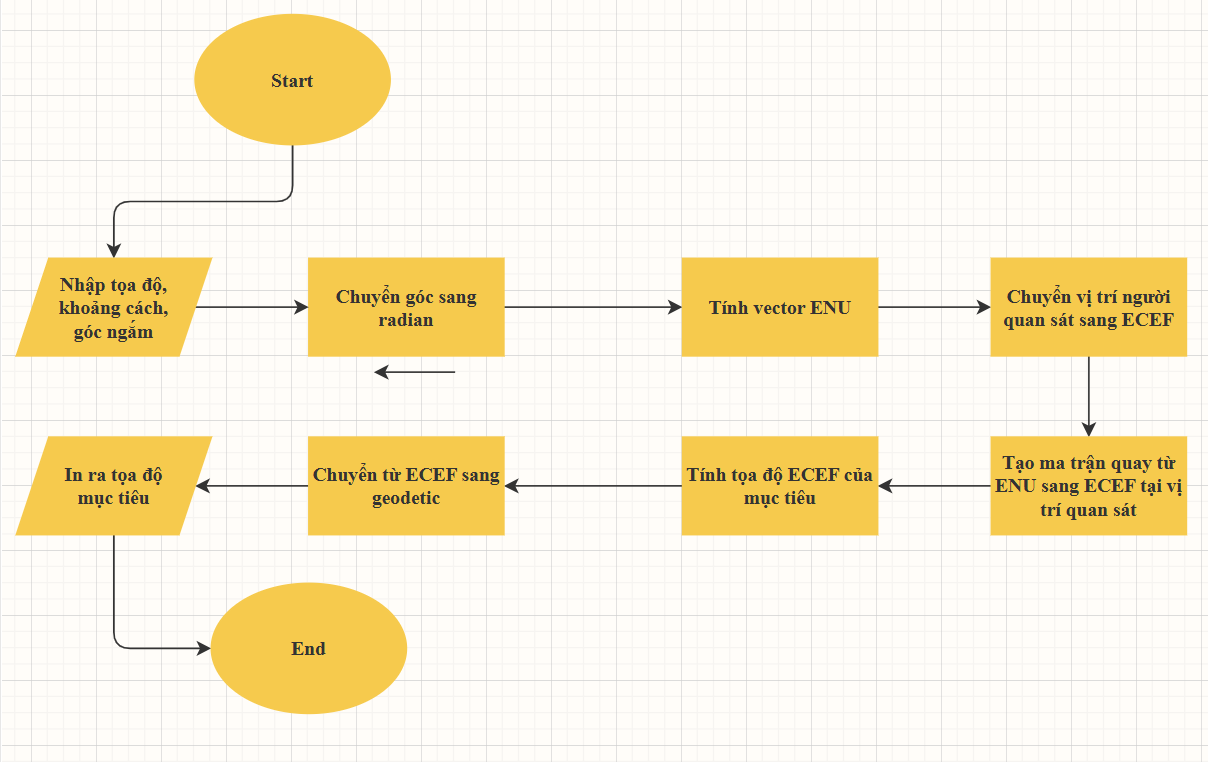
\includegraphics[scale=0.46]{Images/Calc/image.png}
\end{center} 


\item Kết quả tính toán từ Python

\begin{center}
    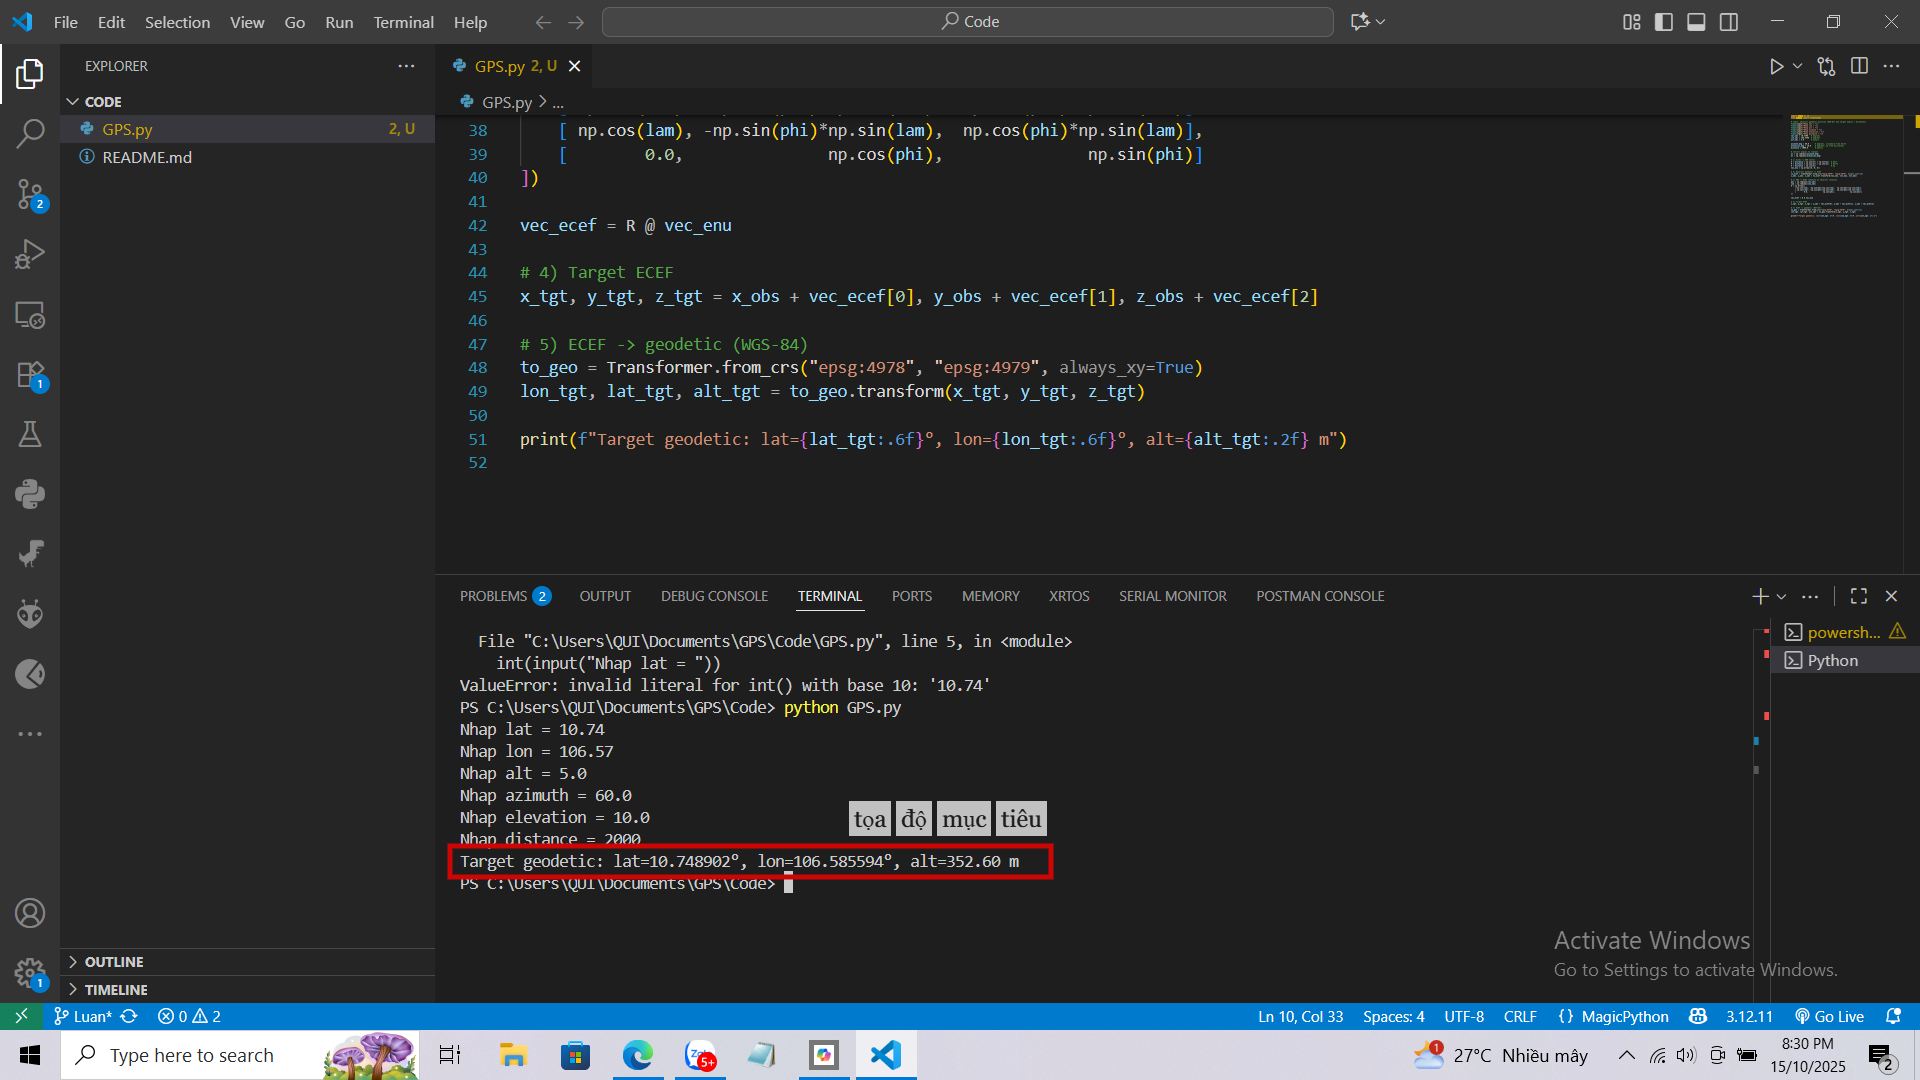
\includegraphics[scale=0.22]{Images/Calc/calcGPS.png}
\end{center}

\newpage
\section{Web Map Use Cases}
\subsection{Tổng quan về Web Map Viewer}
\subsubsection{Định nghĩa về Web Map Viewer}
Web Map Viewer là một ứng dụng hoặc công cụ thực hiện trên nền tảng web cho phép người dùng xem, tương tác và phân tích dữ liệu bản đồ trực tuyến. Trong phạm vi dự án, module này thường được dùng để truy cập các bản đồ và thông tin địa lý, chia sẻ với người khác và tối ưu hóa cho người dùng không chuyên về địa lý.
\subsubsection{Mục tiêu của Web Map Viewer}
\begin{itemize}
    \item Cung cấp giao diện trực quan cho phép xác minh, chia sẻ và xuất tọa độ mục tiêu nhanh chóng (suitable for field operations).
    \item Tích hợp dữ liệu cảm biến (GPS, IMU, laser rangefinder) để chuyển từ đo đạc hướng/khoảng cách sang tọa độ địa lý hiển thị trên bản đồ.
    \item Hỗ trợ đa kịch bản: quân sự, tìm kiếm cứu nạn, trắc địa/GIS, khảo sát xây dựng, quản lý khủng hoảng, nông lâm nghiệp, du lịch, môi trường, hạ tầng, và đào tạo.
    \item Dễ triển khai (static HTML + Leaflet), nhẹ, tương thích trên thiết bị di động và có cơ chế làm việc offline (cached tiles / mbtiles).
\end{itemize}
\subsubsection{Chức năng chính}
Web Map Viewer nên cung cấp một tập hợp chức năng cốt lõi để đáp ứng các use case hiện trường và phân tích sau xử lý:
\begin{itemize}
    \item \textbf{Theo dõi thời gian thực (Real-time Tracking):} hiển thị vị trí observer, team hoặc asset theo timestamp; hỗ trợ streaming vị trí qua WebSocket/HTTP SSE/MQTT.
    \item \textbf{Tích hợp cảm biến (Sensor Integration):} nhận và xử lý trực tiếp dữ liệu GPS, IMU, laser rangefinder (azimuth/elevation/distance), cho phép chuyển đổi hướng + khoảng cách sang tọa độ địa lý và hiển thị trên map.
    \item \textbf{Vẽ, đo đạc và chỉnh sửa không gian (Drawing \& Measurement):} tạo/ sửa marker, polyline, polygon; đo khoảng cách, diện tích; gán thuộc tính metadata cho feature.
    \item \textbf{Quản lý lớp (Layer Management):} bật/tắt layer, điều chỉnh thứ tự hiển thị, thay đổi style/symbol cho từng lớp, hỗ trợ vector và raster tiles.
    \item \textbf{Chuyển đổi hệ toạ độ \& phép chiếu:} hiển thị tọa độ theo nhiều định dạng (DD, DMS), chuyển đổi giữa WGS-84/EPSG:3857/UTM khi cần cho tính toán chính xác.
    \item \textbf{Export/Import dữ liệu:} xuất/nhập GeoJSON, KML, CSV; xuất báo cáo in/PDF và screenshot bản đồ.
    \item \textbf{Offline mode \& caching:} lưu tile/mbtiles cục bộ, lưu tạm các điểm đo, đồng bộ khi có kết nối.
    \item \textbf{Điều hướng và tuyến đường (Routing):} (tuỳ chọn) tính đường đi ngắn nhất, tạo đường dẫn tới điểm đo/target, tích hợp elevation profile cho phân tích địa hình.
    \item \textbf{Alerts, Geofencing \& Notifications:} định nghĩa vùng (geofence) và cảnh báo khi asset vào/ra vùng; gửi cảnh báo tới người dùng/máy chủ.
    \item \textbf{Time slider / Replay:} phát lại lịch sử vị trí theo thời gian để phân tích diễn tiến sự kiện hoặc audit.
    \item \textbf{Bảo mật và phân quyền:} xác thực người dùng, phân quyền theo vai trò, logging hoạt động và chữ ký số cho dữ liệu nhạy cảm.
    \item \textbf{API \& Interoperability:} REST/GraphQL/WebSocket API để tích hợp với hệ thống thứ cấp (backend, command center, database GIS), hỗ trợ xuất dữ liệu cho QGIS/ArcGIS.
\end{itemize}
\subsubsection{Lợi ích khi sử dụng Web Map Viewer}
Sử dụng Web Map Viewer đem lại nhiều lợi ích thiết thực cho các bên liên quan (field operator, analyst, command center, quản lý), cụ thể:
\begin{itemize}
    \item \textbf{Tăng cường nhận thức tình huống (Situational Awareness):} tập hợp và trực quan hoá vị trí, mục tiêu và trạng thái cảm biến giúp người quyết định nắm bắt tình hình nhanh và chính xác hơn.
    \item \textbf{Ra quyết định nhanh hơn và chính xác hơn:} thông tin trực quan, đo đạc tức thời và metadata chất lượng (HDOP, SNR, timestamp) giúp giảm sai sót so với phương pháp thủ công.
    \item \textbf{Hợp tác hiệu quả (Collaboration):} chia sẻ bản đồ/feature/track theo thời gian thực giữa nhiều người dùng, giảm trùng lặp công việc và cải thiện phối hợp tác chiến/ cứu hộ/ khảo sát.
    \item \textbf{Tiết kiệm chi phí và thời gian:} giảm nhu cầu di chuyển lại nhiều lần bằng cách ghi nhận chính xác điểm đo, tái sử dụng dữ liệu; giảm chi phí giấy tờ/hoạt động thủ công.
    \item \textbf{Tính nhất quán và truy vết (Auditability):} lưu lịch sử đo, replay và audit log giúp kiểm chứng thao tác, phục vụ báo cáo hậu kiểm và pháp lý.
    \item \textbf{Khả năng mở rộng và tích hợp:} thiết kế dựa trên chuẩn mở (GeoJSON, REST, EPSG) giúp dễ tích hợp với hệ thống GIS/ERPs khác, mở rộng chức năng khi cần (routing, analytics).
    \item \textbf{Hoạt động trong điều kiện hạn chế kết nối:} chế độ offline và cache cho phép hoạt động trong vùng không có mạng — rất quan trọng cho SAR, công trường, vùng xa.
    \item \textbf{Nâng cao an toàn và tuân thủ:} cơ chế cảnh báo, geofencing và quản lý quyền giúp tuân thủ quy trình an toàn và giảm rủi ro vận hành.
    \item \textbf{Hỗ trợ đào tạo và đánh giá năng lực:} chế độ replay, scoring và record giúp huấn luyện đội ngũ (drills) và đánh giá hiệu năng sau nhiệm vụ.
\end{itemize}
\subsection{Use Cases}
\subsubsection{MILITARY \& DEFENSE}
\textbf{Use case 1.1: Hệ thống kiểm soát hỏa lực pháo binh} \\

\textbf{Scenario:}
\begin{quote}
Một đơn vị pháo binh cần xác định tọa độ mục tiêu để điều chỉnh hỏa lực.
\end{quote}

\textbf{Workflow:}
\begin{enumerate}
    \item \textbf{Observer (Forward Observer)}: Đứng tại vị trí cần quan sát, quan sát mục tiêu
    \item \textbf{Measurement:}
    \begin{itemize}
        \item GPS: Thu thập tọa độ observer
        \item IMU/Compass: Đo góc phương vị đến mục tiêu
        \item Laser Rangefinder: Đo khoảng cách
    \end{itemize}
    \item \textbf{Calculation}: Hệ thống tính tọa độ mục tiêu
    \item \textbf{Visualization}: Hiển thị trên web map
    \item \textbf{Communication}: Chia sẻ liên kết bản đồ HTML với trung tâm kiểm soát hỏa lực
    \item \textbf{Verification}: Verify tọa độ trên map trước khi tiếp cận
\end{enumerate}
\textbf{Web Map Features:}
\begin{itemize}[label=\textbullet]
    \item Cập nhật điểm đánh dấu theo thời gian thực
    \item Hiển thị khoảng cách và phương vị
    \item Hiển thị trực quan đường ngắm
    \item Cửa sổ thông tin tọa độ
    \item Xuất tọa độ cho phần mềm điều khiển hỏa lực
\end{itemize}
\textbf{Benefits:}
\begin{itemize}[label=\textbullet]
    \item \textbf{Accuracy}: Visual verification trước khi bắn
    \item \textbf{Speed}: Chia sẻ tọa độ tức thì
    \item \textbf{Mobility}: Hoạt động trên tablet/phone trong field
    \item \textbf{Offline}: Không cần kết nối Internet
\end{itemize}
\textbf{Screenshot Example:}
\begin{verbatim}
[Observer Marker] ----2.5km----> [Target Marker]
    (Green)                           (Red)


Popup Info:
Observer: 10.762622°, 106.660172°
Target: 10.784523°, 106.683421°
Bearing: 45° (NE)
Distance: 2.5km
Elevation: +15° (target above observer)
\end{verbatim}
\textbf{Use case 1.2: Chỉ định mục tiêu UAV/Drone} \\

\textbf{Scenario:}
\begin{quote}
UAV operator cần designate target cho surveillance hoặc strike mission.
\end{quote}

\textbf{Workflow:}
\begin{enumerate}
    \item Người điều khiển UAV xác định mục tiêu trực quan
    \item Ghi lại vị trí GPS + góc gimbal
    \item Tính toán tọa độ mục tiêu
    \item Hiển thị trên bản đồ web với đường bay
    \item Chia sẻ bản đồ với trung tâm chỉ huy
    \item Cập nhật trạng thái mục tiêu theo thời gian thực
\end{enumerate}
\textbf{Web Map Features:}
\begin{itemize}[label=\textbullet]
    \item Nhiều mục tiêu trên một bản đồ
    \item Đánh dấu mã màu (mức độ đe dọa)
    \item Lớp phủ đường bay
    \item Cập nhật vị trí theo thời gian thực
    \item Chỉ báo mức độ ưu tiên của mục tiêu
\end{itemize}
\textbf{Benefits:}
\begin{itemize}[label=\textbullet]
    \item \textbf{Situational Awareness}: Xem tất cả mục tiêu trên một bản đồ
    \item \textbf{Real-time Updates}: Theo dõi mục tiêu động
    \item \textbf{Precision}: Xác minh tọa độ trước khi giao chiếnt
\end{itemize}
\subsubsection{Search \& Rescue (SAR)}
\textbf{Use case 2.1: Vị trí người mất tích} \\

\textbf{Scenario:}
\begin{quote}
Đội SAR cần xác định vị trí người mất tích trong rừng/núi.
\end{quote}

\textbf{Workflow:}
\begin{enumerate}
    \item \textbf{Initial Report}: Nhận tọa độ vị trí cuối cùng được biết đến
    \item \textbf{Search Pattern}: Chia khu vực thành các sectors
    \item \textbf{Team Deployment}: Mỗi đội báo cáo vị trí + tìm kiếm
    \item \textbf{Target Spotted}: Đội báo cáo azimuth/distance đến subject
    \item \textbf{Coordinate Calculation}: Tính toán vị trí chính xác
    \item \textbf{Web Map Update}: Đánh dấu vị trí, chia sẻ với tất cả teams
    \item \textbf{Rescue Coordination}: Điều dẫn đội ngũ y tế đến địa điểm chính xác
\end{enumerate}
\textbf{Web Map Features:}
\begin{itemize}[label=\textbullet]
    \item Đánh dấu nhiều đội (nhiều màu khác nhau)
    \item Lớp phủ khu vực tìm kiếm
    \item Vòng tròn khoảng cách (bán kính tìm kiếm)
    \item Tùy chọn bản đồ địa hình
    \item Đánh dấu vị trí cuối cùng được biết đến
\end{itemize}
\textbf{Benefits:}
\begin{itemize}[label=\textbullet]
    \item \textbf{Time Critical}: Nhanh chóng phối hợp các nỗ lực cứu hộ
    \item \textbf{Precision}: Vị trí chính xác để sơ tán y tế
    \item \textbf{Coordination}: Tất cả các đội đều nhìn thấy cùng một bản đồ
    \item \textbf{Offline Maps}: Làm việc trong vùng không có vùng phủ sóng di động
\end{itemize}
\textbf{Use case 2.2: Maritime Search \& Rescue} \\

\textbf{Scenario:}
\begin{quote}
Coast guard tìm kiếm tàu gặp nạn trên biển.
\end{quote}

\textbf{Workflow:}
\begin{enumerate}
    \item Tín hiệu cấp cứu được nhận với tọa độ gần đúng
    \item Tàu/máy bay được triển khai đến khu vực tìm kiếm
    \item Quan sát bằng mắt thường: Ghi lại hướng/khoảng cách từ tàu
    \item Tính toán tọa độ hiệu chỉnh độ trôi
    \item Bản đồ web hiển thị:
    \begin{itemize}
        \item vị trí tàu tìm kiếm
        \item vị trí cuối cùng được biết của mục tiêu
        \item vị trí hiện tại
        \item Đường đi dự đoán trôi dạt
    \end{itemize}
    \item Phối hợp các hoạt động cứu hộ
\end{enumerate}
\textbf{Web Map Features:}
\begin{itemize}[label=\textbullet]
    \item Tỷ lệ hải lý
    \item Lớp phủ dòng chảy/gió (nếu có)
    \item Hình ảnh hóa mẫu tìm kiếm
    \item Đánh dấu vị trí có dấu thời gian
\end{itemize}
\subsubsection{Tourism \& Recreation}
\textbf{Use case 3.1: Điều hướng đường mòn} \\

\textbf{Scenario:}
\begin{quote}
Người đi bộ sử dụng hệ thống để điều hướng và đánh dấu các điểm ưa thích.
\end{quote}

\textbf{Workflow:}
\begin{enumerate}
    \item Bắt đầu đi bộ đường dài: ghi lại GPS điểm đầu đường mòn
    \item Đánh dấu các điểm dừng dọc đường mòn
    \item Ghi chú các điểm thú vị (điểm ngắm cảnh, khu cắm trại)
    \item Tính toán khoảng cách giữa các điểm
    \item Chia sẻ bản đồ đường mòn với những người đi bộ đường dài khác
    \item Tải lên cơ sở dữ liệu đường mòn
\end{enumerate}
\textbf{Web Map Features:}
\begin{itemize}[label=\textbullet]
    \item Lớp phủ đường mòn
    \item Độ cao (nếu có)
    \item Điểm đánh dấu ảnh
    \item Tạo liên kết chia sẻ
\end{itemize}
\subsubsection{Education \& Training}
\textbf{Use case 4.1: Bài tập huấn luyện quân sự} \\

\textbf{Scenario:}
\begin{quote}
Huấn luyện quân đội về quy trình chỉ định mục tiêu.
\end{quote}

\textbf{Workflow:}
\begin{enumerate}
    \item Giảng viên thiết lập kịch bản đào tạo
    \item Học viên thực hành đo mục tiêu
    \item Gửi tọa độ qua giao diện web
    \item Hệ thống tính toán độ chính xác
    \item Bản đồ web hiển thị tất cả bài nộp của học viên so với thực tế
    \item Tóm tắt với phân tích trực quan
\end{enumerate}
\textbf{Web Map Features:}
\begin{itemize}[label=\textbullet]
    \item Nhiều người dùng gửi bài
    \item Hiển thị lỗi (khoảng cách so với thực tế)
    \item Hệ thống chấm điểm
    \item Khả năng phát lại
\end{itemize}
\subsection{Technical Architecture}
\subsubsection{System Components}

\begin{center}
    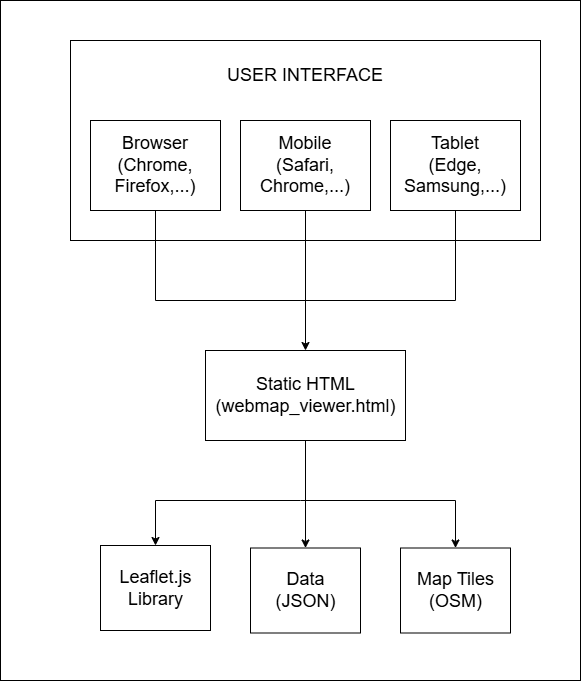
\includegraphics[scale=0.5]{Images/webmap_system_components.png}
\end{center}

\subsubsection{Technology Stack}
\paragraph{Frontend}
\begin{itemize}[label=\textbullet]
    \item \textbf{HTML5}: Structure \& semantics
    \item \textbf{CSS3}: Styling \& responsive design
    \item \textbf{JavaScript ES6}: Logic \& interactivity
    \item \textbf{Leaflet.js 1.9.4}: Mapping engine
\end{itemize}
\paragraph{Data Formats}
\begin{itemize}[label=\textbullet]
    \item \textbf{GeoJSON}: Geographic data exchange
    \item \textbf{JSON}: Configuration \& metadata
    \item \textbf{CSV}: Bulk data import/export
\end{itemize}
\paragraph{Map Services}
\begin{itemize}[label=\textbullet]
    \item \textbf{OpenStreetMap}: Base map tiles
    \item \textbf{Alternatives}: Stamen Terrain, CartoDB, Mapbox
\end{itemize}
\end{itemize}

\newpage
\subsection{Prototype phần mềm mô phỏng (Leaflet Web Map)}
\textbf{Trang web triển khai:} \href{https://kzeyrox45.github.io/GPS-Target-Calculating-System/}{kzeyrox45.github.io/GPS-Target-Calculating-System}
\subsubsection{Mục tiêu}
Phần mềm mô phỏng được xây dựng nhằm trực quan hoá kết quả tính toán toạ độ mục tiêu từ dữ liệu đo (toạ độ người quan sát, góc ngắm và khoảng cách). 
Giao diện cho phép người dùng nhập thông tin đầu vào, tính toán toạ độ mục tiêu và hiển thị kết quả ngay trên bản đồ thực tế, giúp dễ dàng kiểm chứng tính chính xác của mô hình.

\subsubsection{Công nghệ sử dụng}
\begin{itemize}
    \item \textbf{HTML, CSS, JavaScript:} Xây dựng giao diện người dùng và xử lý sự kiện nhập liệu.
    \item \textbf{Leaflet.js:} Thư viện bản đồ mã nguồn mở, hiển thị bản đồ nền (OpenStreetMap) và các marker.
    \item \textbf{OpenStreetMap (OSM):} Nguồn dữ liệu bản đồ miễn phí được Leaflet sử dụng.
\end{itemize}

\subsubsection{Cấu trúc giao diện}
Giao diện chính của hệ thống được chia thành hai phần:
\begin{enumerate}
    \item \textbf{Khung nhập dữ liệu:} Bao gồm các trường nhập
    \begin{itemize}
        \item Toạ độ người quan sát (vĩ độ, kinh độ).
        \item Góc ngắm (đơn vị độ, tính từ hướng Bắc).
        \item Khoảng cách tới mục tiêu (đơn vị km).
    \end{itemize}
    \item \textbf{Bản đồ hiển thị:} Hiển thị vị trí người quan sát, mục tiêu và hướng ngắm.
\end{enumerate}

\noindent
Các phần tử trên bản đồ gồm:
\begin{itemize}
    \item Marker màu đỏ : vị trí người quan sát.
    \item Marker màu xanh : vị trí mục tiêu được tính toán.
    \item Đường đứt nét (--): biểu diễn hướng ngắm.
    \item Khung chú giải: hiển thị ý nghĩa các ký hiệu.
\end{itemize}


\begin{figure}[H]
    \centering
    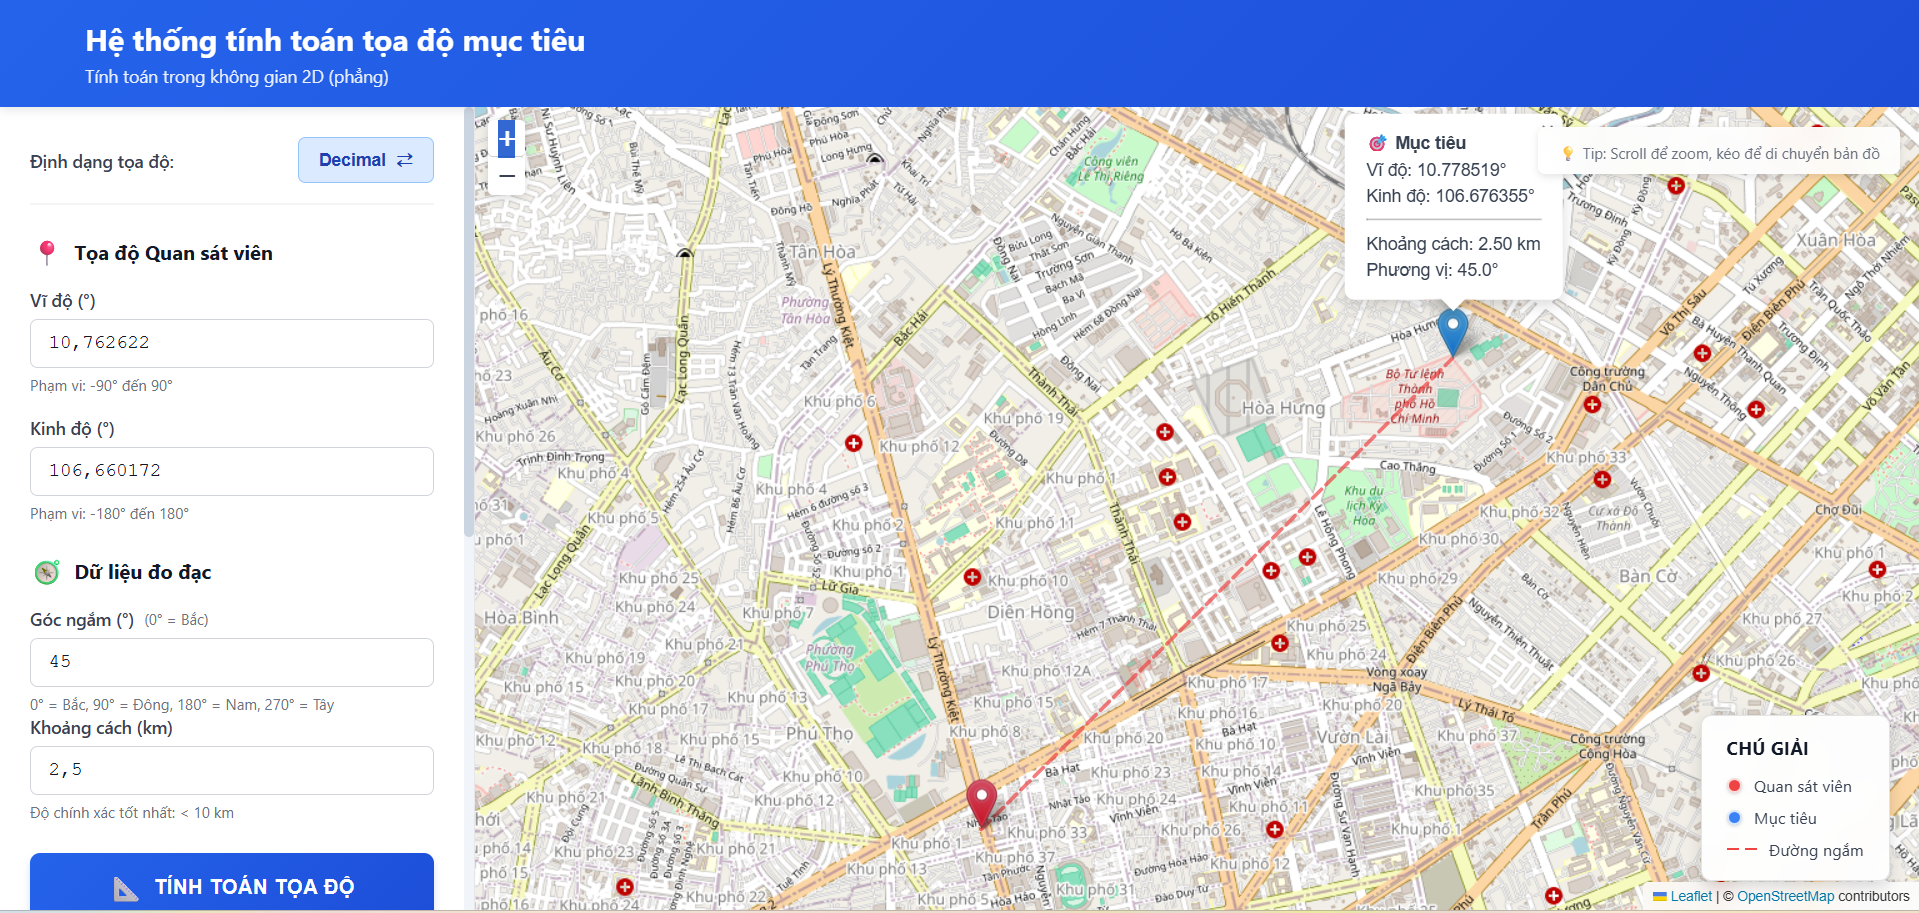
\includegraphics[scale=0.3]
    {Images/webmap_interface.png}
    \vspace{0.8cm} 
    \caption{Giao diện hệ thống tính toán toạ độ mục tiêu trên bản đồ Leaflet}
\end{figure}

\newpage

Hệ thống cho phép người dùng lựa chọn định dạng nhập tọa độ ở hai dạng phổ biến là \textbf{Decimal} (độ thập phân) và \textbf{DMS} (Degrees–Minutes–Seconds, tức độ–phút–giây). 
Người dùng có thể chuyển đổi linh hoạt giữa hai định dạng thông qua nút “\textit{Định dạng tọa độ: DMS và Decimal}”, giúp thuận tiện trong việc nhập liệu theo các nguồn dữ liệu đo đạc khác nhau.

\begin{figure}[H]
    \centering
    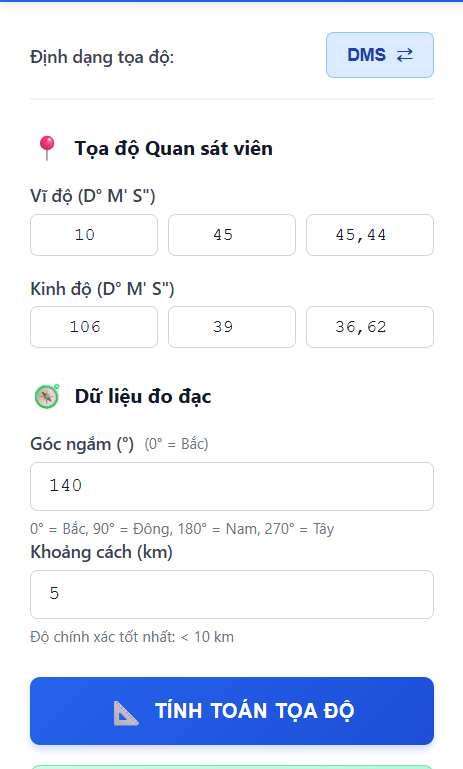
\includegraphics[scale=0.33]
    {Images/webmap_interface_dms.png}
    \vspace{0.8cm} 
    \caption{Giao diện hệ thống tính toán toạ độ mục tiêu trên bản đồ Leaflet}
\end{figure}

\subsubsection{Nguyên lý hoạt động}
Khi người dùng nhập các thông số đầu vào, hệ thống sẽ:
\begin{enumerate}
    \item Lấy dữ liệu toạ độ người quan sát $(lat_1, lon_1)$, góc ngắm $\theta$ và khoảng cách $d$.
    \item Thực hiện phép tính toạ độ mục tiêu theo mô hình toạ độ cực.
    \item Hiển thị vị trí người quan sát và mục tiêu trên bản đồ OpenStreetMap thông qua Leaflet và bảng dữ liệu chi tiết.
\end{enumerate}

\subsubsection{Kết quả mô phỏng}
Sau khi nhập dữ liệu và nhấn nút \textit{“Tính toán toạ độ”}, hệ thống hiển thị kết quả trực tiếp trên bản đồ:
\begin{itemize}
    \item Toạ độ mục tiêu được hiển thị bằng marker màu xanh.
    \item Hướng ngắm được thể hiện bằng đoạn thẳng nối hai vị trí.
    \item Thông tin chi tiết của từng điểm được hiển thị khi người dùng rê chuột vào marker, hoặc kéo xuống và xem bảng "Tọa độ Mục tiêu"
\end{itemize}

\begin{figure}[H]
    \centering
    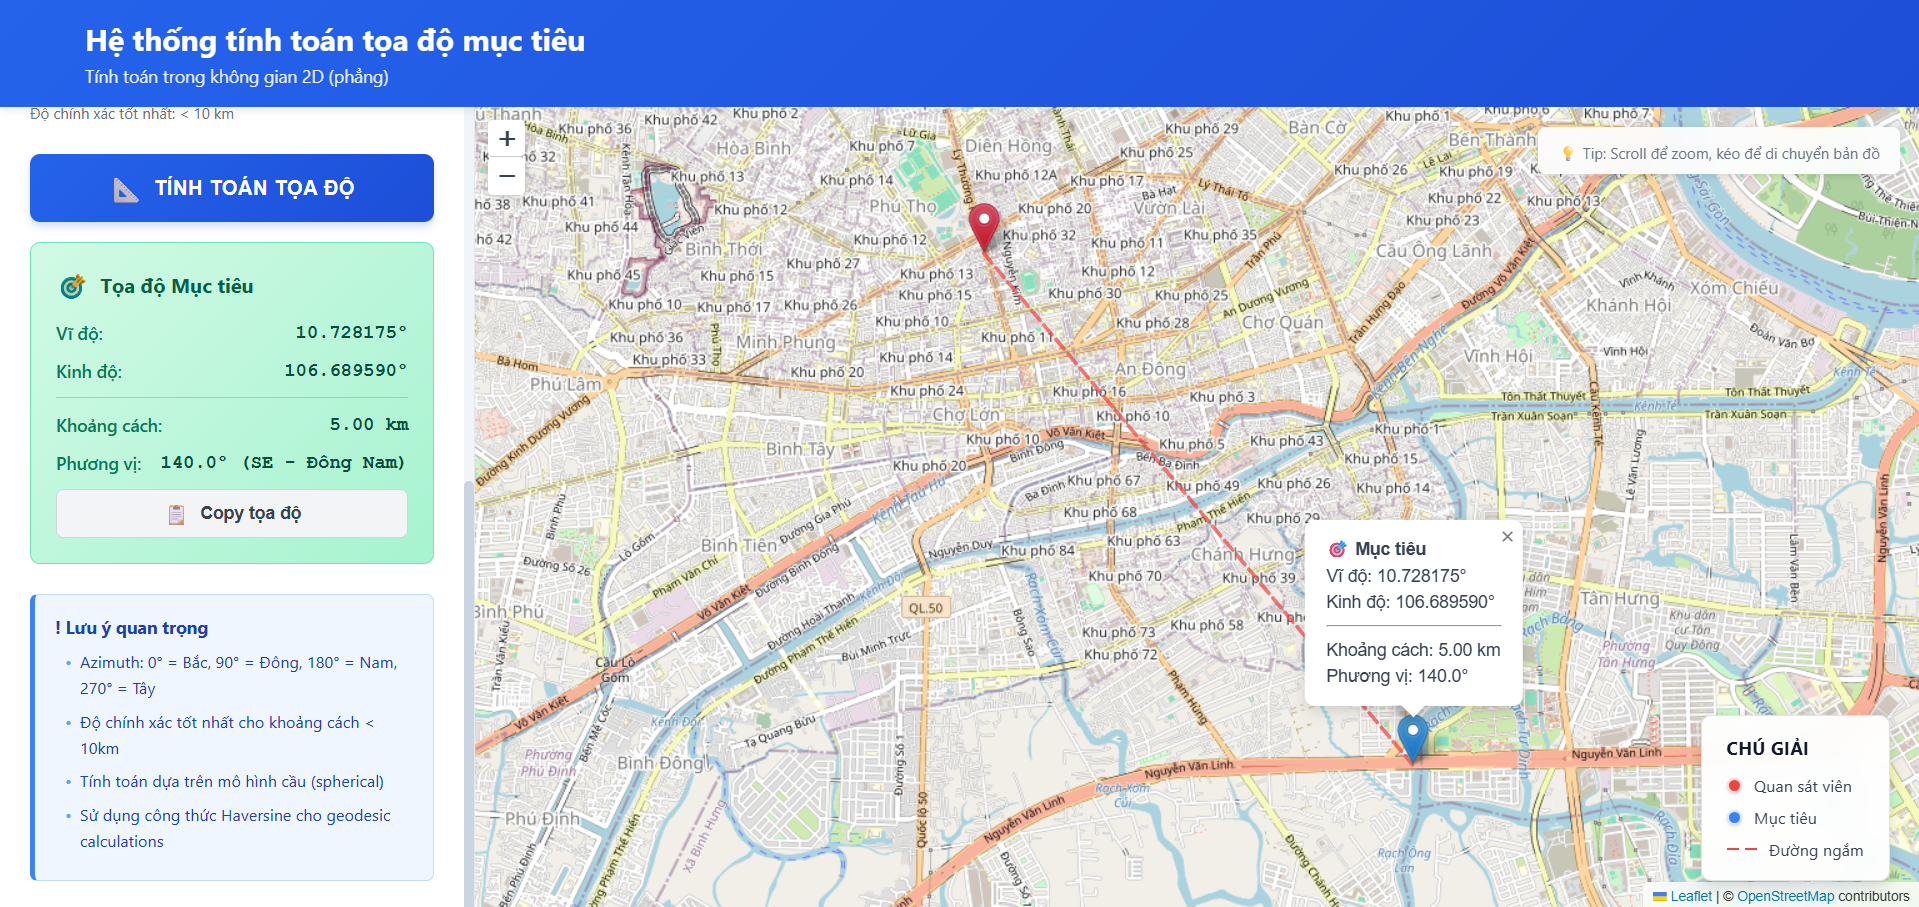
\includegraphics[scale=0.33]
    {Images/webmap_result.png}
    \vspace{0.8cm} 
    \caption{Giao diện hệ thống tính toán toạ độ mục tiêu trên bản đồ Leaflet}
\end{figure}

\subsubsection{Đánh giá}
Prototype phần mềm mô phỏng đã đáp ứng yêu cầu trực quan hoá kết quả tính toán, giúp người dùng dễ dàng xác định vị trí mục tiêu trong không gian phẳng 2D. 
Hệ thống có thể mở rộng để làm việc với bản đồ 3D hoặc kết nối với cơ sở dữ liệu cảm biến thực tế trong các nghiên cứu tiếp theo.

\newpage
\section{Yêu cầu về hệ thống}

\subsection{Yêu cầu chức năng}
Hệ thống tính toán tọa độ mục tiêu cần đáp ứng các yêu cầu chức năng sau:

\subsubsection{Nhập dữ liệu quan sát}
\begin{itemize}
    \item \textbf{RF-01}: Hệ thống phải cho phép người dùng nhập tọa độ người quan sát dưới hai định dạng:
    \begin{itemize}
        \item Decimal Degrees (DD): Vĩ độ và kinh độ dạng thập phân (ví dụ: 10.762622°, 106.660172°).
        \item Degrees Minutes Seconds (DMS): Vĩ độ và kinh độ dạng độ-phút-giây (ví dụ: 10° 45' 45.44", 106° 39' 36.62").
    \end{itemize}
    \item \textbf{RF-02}: Hệ thống phải hỗ trợ chuyển đổi tự động giữa hai định dạng tọa độ (DD $\leftrightarrow$ DMS) mà không làm mất dữ liệu.
    \item \textbf{RF-03}: Hệ thống phải cho phép nhập góc phương vị (Azimuth) từ 0° đến 360°, với 0° là hướng Bắc địa lý.
    \item \textbf{RF-04}: Hệ thống phải cho phép nhập khoảng cách đến mục tiêu (Distance) tính bằng kilômét, với giá trị dương.
\end{itemize}

\subsubsection{Validation dữ liệu đầu vào}
\begin{itemize}
    \item \textbf{RF-05}: Hệ thống phải kiểm tra tính hợp lệ của tọa độ:
    \begin{itemize}
        \item Vĩ độ: $-90° \leq \phi \leq 90°$
        \item Kinh độ: $-180° \leq \lambda \leq 180°$
    \end{itemize}
    \item \textbf{RF-06}: Hệ thống phải kiểm tra góc phương vị: $0° \leq \theta \leq 360°$
    \item \textbf{RF-07}: Hệ thống phải kiểm tra khoảng cách: $d > 0$ km
    \item \textbf{RF-08}: Hệ thống phải hiển thị thông báo lỗi rõ ràng khi dữ liệu đầu vào không hợp lệ.
    \item \textbf{RF-09}: Hệ thống phải cảnh báo người dùng khi khoảng cách lớn hơn 100 km về khả năng sai số tăng cao do sử dụng mô hình cầu.
\end{itemize}

\subsubsection{Tính toán tọa độ mục tiêu}
\begin{itemize}
    \item \textbf{RF-10}: Hệ thống phải tính toán tọa độ mục tiêu sử dụng công thức Haversine \cite{sinnot1984virtues} trên mô hình cầu với bán kính Trái Đất $R = 6371$ km.
    \item \textbf{RF-11}: Hệ thống phải cung cấp kết quả tọa độ mục tiêu với độ chính xác tối thiểu 6 chữ số thập phân (tương đương ~0.1 mét).
    \item \textbf{RF-12}: Hệ thống phải tính toán ngược lại khoảng cách và góc phương vị từ tọa độ kết quả để xác minh độ chính xác (verification).
    \item \textbf{RF-13}: Hệ thống phải ước lượng sai số tổng hợp dựa trên các nguồn sai số từ GPS, góc phương vị và khoảng cách.
\end{itemize}

\subsubsection{Hiển thị kết quả trên bản đồ}
\begin{itemize}
    \item \textbf{RF-14}: Hệ thống phải hiển thị vị trí người quan sát và mục tiêu trên bản đồ tương tác sử dụng thư viện Leaflet.js \cite{leafletjs}.
    \item \textbf{RF-15}: Hệ thống phải sử dụng marker khác màu để phân biệt:
    \begin{itemize}
        \item Marker đỏ: Vị trí người quan sát
        \item Marker xanh: Vị trí mục tiêu
    \end{itemize}
    \item \textbf{RF-16}: Hệ thống phải vẽ đường nối (bearing line) giữa người quan sát và mục tiêu để trực quan hóa hướng ngắm.
    \item \textbf{RF-17}: Hệ thống phải tự động điều chỉnh mức zoom và vị trí trung tâm bản đồ (fitBounds) để hiển thị cả hai điểm trong khung nhìn.
    \item \textbf{RF-18}: Hệ thống phải hiển thị popup thông tin chi tiết khi người dùng click vào marker, bao gồm tọa độ, khoảng cách và góc phương vị.
\end{itemize}

\subsubsection{Xuất và chia sẻ dữ liệu}
\begin{itemize}
    \item \textbf{RF-19}: Hệ thống phải cho phép sao chép (copy) tọa độ mục tiêu vào clipboard.
    \item \textbf{RF-20}: Hệ thống phải hiển thị thông tin kết quả dưới dạng văn bản có cấu trúc, dễ đọc.
\end{itemize}

\subsection{Yêu cầu phi chức năng}

\subsubsection{Hiệu năng}
\begin{itemize}
    \item \textbf{NFR-01}: Thời gian tính toán tọa độ mục tiêu phải nhỏ hơn 100ms trên thiết bị có cấu hình trung bình.
    \item \textbf{NFR-02}: Thời gian render bản đồ và marker phải nhỏ hơn 500ms sau khi nhận được kết quả tính toán.
    \item \textbf{NFR-03}: Hệ thống phải hoạt động mượt mà với tần suất cập nhật tối đa 10 lần/giây (cho trường hợp tích hợp cảm biến thời gian thực trong tương lai).
\end{itemize}

\subsubsection{Khả năng sử dụng (Usability)}
\begin{itemize}
    \item \textbf{NFR-04}: Giao diện người dùng phải trực quan, dễ sử dụng cho người không chuyên về GIS.
    \item \textbf{NFR-05}: Hệ thống phải hỗ trợ phím tắt:
    \begin{itemize}
        \item Enter: Thực hiện tính toán
        \item Ctrl+M: Chuyển đổi định dạng tọa độ
        \item Ctrl+C: Sao chép kết quả (khi đang hiển thị)
    \end{itemize}
    \item \textbf{NFR-06}: Thông báo lỗi phải rõ ràng, hướng dẫn người dùng cách khắc phục.
    \item \textbf{NFR-07}: Giao diện phải responsive, hoạt động tốt trên màn hình từ 320px đến 1920px.
\end{itemize}

\subsubsection{Tương thích}
\begin{itemize}
    \item \textbf{NFR-08}: Hệ thống phải tương thích với các trình duyệt hiện đại:
    \begin{itemize}
        \item Chrome/Edge (phiên bản 90+)
        \item Firefox (phiên bản 88+)
        \item Safari (phiên bản 14+)
    \end{itemize}
    \item \textbf{NFR-09}: Hệ thống phải hoạt động trên cả thiết bị desktop và mobile (iOS, Android).
    \item \textbf{NFR-10}: Hệ thống phải sử dụng chuẩn WGS-84 \cite{wgs84} để đảm bảo tương thích với các hệ thống GPS toàn cầu.
\end{itemize}

\subsubsection{Bảo trì và mở rộng}
\begin{itemize}
    \item \textbf{NFR-11}: Mã nguồn phải được tổ chức theo kiến trúc module rõ ràng:
    \begin{itemize}
        \item Module tính toán (coordinateCalculator.js)
        \item Module hiển thị bản đồ (mapViewer.js)
        \item Module giao diện (index.html, style.css)
    \end{itemize}
    \item \textbf{NFR-12}: Mã nguồn phải có comment đầy đủ, tuân thủ chuẩn JSDoc cho JavaScript.
    \item \textbf{NFR-13}: Hệ thống phải dễ dàng mở rộng để tích hợp:
    \begin{itemize}
        \item Backend API trong tương lai
        \item Thuật toán tính toán chính xác hơn (Vincenty, Karney \cite{karney2013algorithms})
        \item Dữ liệu độ cao (Elevation API)
    \end{itemize}
\end{itemize}

\subsubsection{Độ tin cậy}
\begin{itemize}
    \item \textbf{NFR-14}: Hệ thống phải xử lý gracefully các trường hợp ngoại lệ (exception handling) mà không bị crash.
    \item \textbf{NFR-15}: Hệ thống phải hoạt động offline sau khi đã tải trang lần đầu (không cần kết nối Internet để tính toán).
    \item \textbf{NFR-16}: Bản đồ nền (OpenStreetMap tiles) phải có cơ chế fallback khi không tải được.
\end{itemize}

\subsubsection{Bảo mật}
\begin{itemize}
    \item \textbf{NFR-17}: Hệ thống không được lưu trữ dữ liệu nhạy cảm trên trình duyệt (localStorage, cookies) trong phiên bản hiện tại.
    \item \textbf{NFR-18}: Hệ thống phải sử dụng HTTPS khi triển khai trên môi trường production.
    \item \textbf{NFR-19}: Mã nguồn phải được kiểm tra bảo mật cơ bản (XSS, injection) trước khi triển khai.
\end{itemize}
\newpage
\section{Đặc tả chi tiết Web hệ thống GPS Target Calculating System}
\begin{figure}[H]
    \centering
    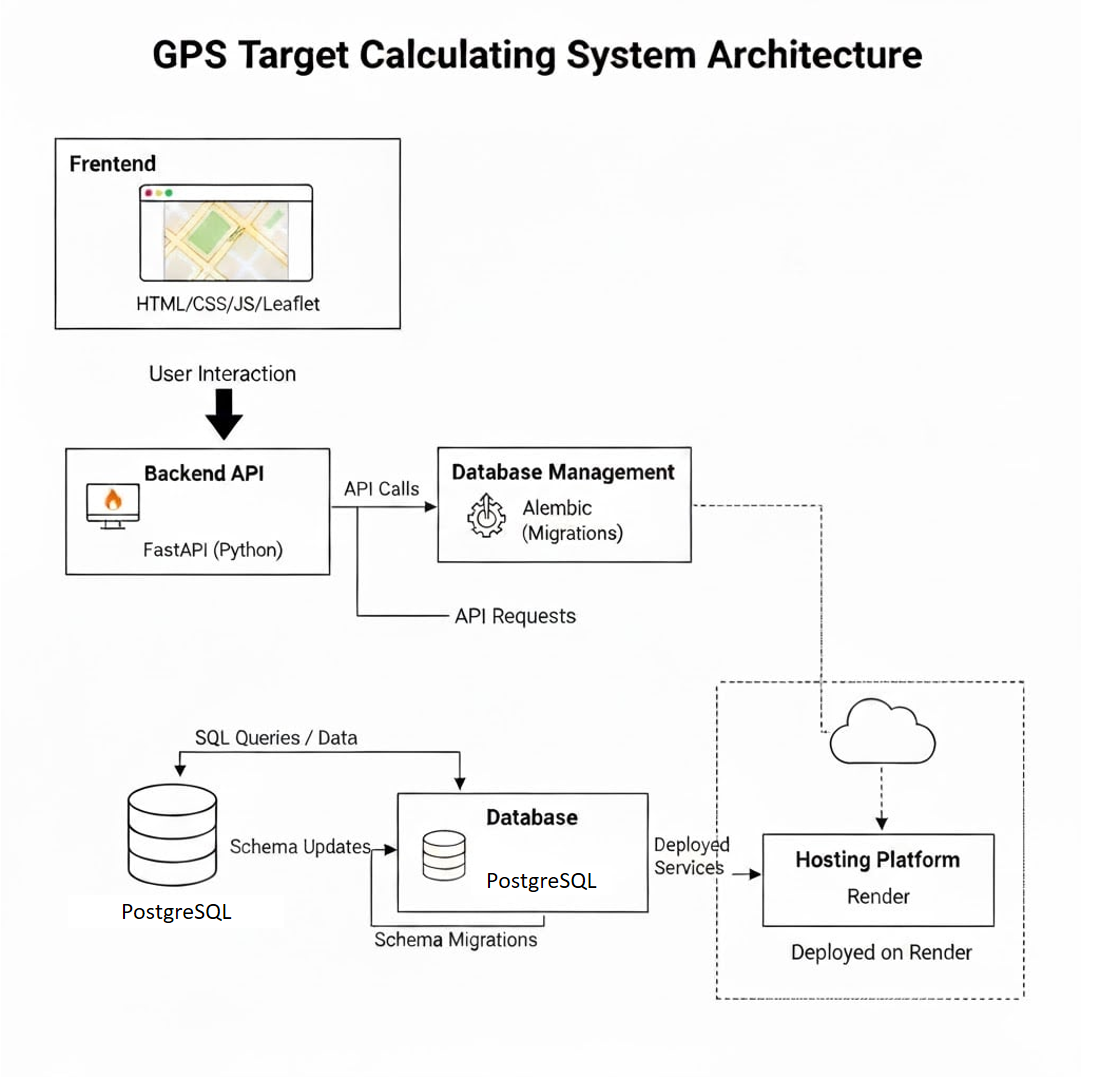
\includegraphics[scale=0.5]
    {Images/WebAr.png}
    \vspace{0.3cm} 
    \caption{Kiến trúc prototype của Web}
\end{figure}

\subsection{Tổng quan}
Hệ thống GPS Target Calculating System được thiết kế để tính toán và hiển thị vị trí mục tiêu dựa trên tọa độ người quan sát, góc ngắm và khoảng cách. Hệ thống bao gồm bốn thành phần chính: Frontend, Backend API, Database và Hosting Platform.
\subsection{Frontend (Giao diện người dùng)}
\begin{itemize}
    \item Công nghệ sử dụng: HTML, CSS, JavaScript, Leaflet.
    \item Chức năng chính:
    \begin{itemize}
        \item Hiển thị bản đồ tương tác bằng thư viện Leaflet.
        \item Cho phép người dùng nhập dữ liệu: tọa độ quan sát viên, góc ngắm, khoảng cách.
        \item Gửi dữ liệu này đến Backend API thông qua các lệnh gọi fetch() hoặc axios.
        \item Nhận kết quả tọa độ mục tiêu từ API và hiển thị marker trên bản đồ.
    \end{itemize}
    \item Đây là nơi người dùng trực tiếp thao tác; mọi tính toán phức tạp được ẩn đi và chỉ trả về kết quả trực quan.
\end{itemize}
\newpage
\subsection{Backend (FastAPI)}
\begin{itemize}
    \item Công nghệ sử dụng: Python, FastAPI.
    \item Cấu trúc chính:
    \begin{itemize}
        \item main.py: điểm khởi chạy ứng dụng, cấu hình CORS, đăng ký router.
        \item routers/calculate.py: định nghĩa endpoint /api/calculate để nhận dữ liệu và trả kết quả.
        \item models.py: định nghĩa bảng dữ liệu (Observation).
        \item schemas.py: định nghĩa input/output bằng Pydantic.
        \item database.py: cấu hình kết nối PostgreSQL.
        \item crud.py: các hàm thao tác với database.
    \end{itemize}
    \item Chức năng chính:
    \begin{itemize}
        \item Nhận dữ liệu từ FE (tọa độ, góc, khoảng cách).
        \item Tính toán tọa độ mục tiêu bằng công thức toán học.
        \item Lưu dữ liệu vào Database.
        \item Trả kết quả về cho FE qua JSON.
    \end{itemize}
    \item Đây là “bộ não” của hệ thống, xử lý logic nghiệp vụ và kết nối dữ liệu.
\end{itemize}

\subsection{Database (PostgreSQL + Alembic)}
\begin{itemize}
    \item Công nghệ sử dụng: PostgreSQL, Alembic (migration).
    \item Chức năng chính:
    \begin{itemize}
        \item Lưu trữ dữ liệu quan sát: vị trí quan sát viên, góc, khoảng cách, tọa độ mục tiêu, thời gian.
        \item Hỗ trợ kiểu dữ liệu không gian (qua PostGIS) để tính toán địa lý chính xác.
        \item Alembic quản lý migration, đảm bảo schema database nhất quán khi phát triển.
    \end{itemize}
    \item Đây là nơi lưu giữ toàn bộ dữ liệu, phục vụ cho việc phân tích, thống kê hoặc hiển thị lại lịch sử.
\end{itemize}

\subsection{Hosting Platform (Render)}
\begin{itemize}
    \item Công nghệ sử dụng: Render Cloud.
    \item Chức năng chính:
    \begin{itemize}
        \item Deploy Backend FastAPI thành một Web Service có URL public.
        \item Cung cấp PostgreSQL Database dưới dạng dịch vụ cloud.
        \item Quản lý môi trường (environment variables), build, start command.
    \end{itemize}
    \item Giúp hệ thống chạy online, người dùng có thể truy cập từ bất kỳ đâu.
\end{itemize}

\subsection{Luồng dữ liệu trong hệ thống}
\begin{itemize}
    \item Người dùng nhập dữ liệu trên Frontend (tọa độ, góc, khoảng cách).
    \item FE gửi request đến Backend API qua endpoint /api/calculate.
    \item Backend xử lý tính toán, lưu dữ liệu vào PostgreSQL.
    \item Kết quả (tọa độ mục tiêu) được trả về FE.
    \item FE hiển thị marker mục tiêu trên bản đồ Leaflet.
\end{itemize}
\newpage
\section{Chi tiết Hiện thực và Phân tích Mã nguồn}

Phần này trình bày chi tiết về cách hệ thống được hiện thực, phân tích các module chính, design patterns được áp dụng, và các quyết định kỹ thuật quan trọng.

\subsection{Kiến trúc Chi tiết}

\subsubsection{Mô hình MVC biến thể}
Hệ thống áp dụng mô hình MVC (Model-View-Controller) biến thể phù hợp với client-side JavaScript:

\begin{verbatim}
Model (coordinateCalculator.js)
  |-- Pure functions (stateless)
  |-- Business logic
  +-- Data transformations

View (index.html + style.css)
  |-- HTML structure
  |-- CSS styling
  +-- Leaflet map rendering

Controller (mapViewer.js)
  |-- Event handlers
  |-- UI state management
  +-- Coordination between Model and View
\end{verbatim}

\textbf{Lợi ích}:
\begin{itemize}
    \item Separating concerns: Mỗi module một trách nhiệm
    \item Testability: Model có thể test độc lập
    \item Maintainability: Thay đổi UI không ảnh hưởng business logic
    \item Reusability: Model có thể tái sử dụng cho CLI, mobile app
\end{itemize}

\subsubsection{Data Flow Architecture}

\begin{figure}[H]
\centering
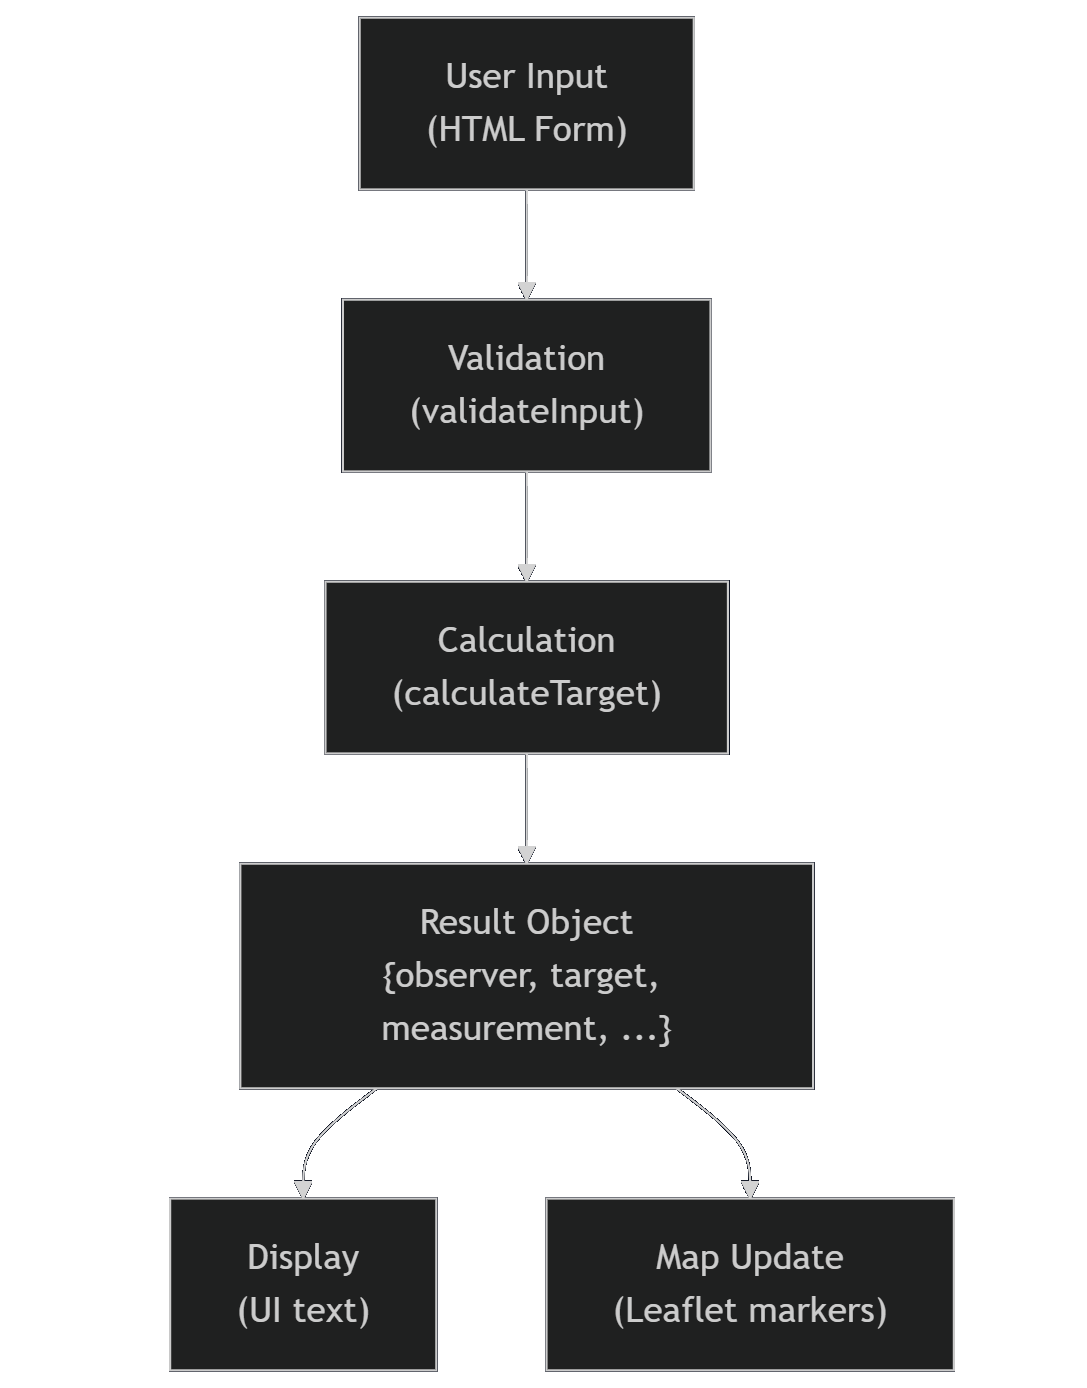
\includegraphics[width=0.6\textwidth]{Images/data_flow_architecture.png}
\caption{Luồng dữ liệu trong hệ thống}
\end{figure}

Luồng dữ liệu một chiều (unidirectional) giúp:
\begin{itemize}
    \item Dễ debug: Trace được data từ input đến output
    \item Predictable: Cùng input $\rightarrow$ cùng output
    \item No side effects: Functions không modify global state
\end{itemize}

\subsection{Module coordinateCalculator.js - Phân tích Chi tiết}

\subsubsection{Constants và Configuration}
Module bắt đầu với định nghĩa constants:

\begin{lstlisting}[language=JavaScript, caption={Constants definition}]
const EARTH_RADIUS_KM = 6371.0;
const DEG_TO_RAD = Math.PI / 180;
const RAD_TO_DEG = 180 / Math.PI;

const LAT_MIN = -90;
const LAT_MAX = 90;
const LON_MIN = -180;
const LON_MAX = 180;
const AZIMUTH_MIN = 0;
const AZIMUTH_MAX = 360;
\end{lstlisting}

\textbf{Design decision}:
\begin{itemize}
    \item UPPER\_CASE naming convention cho constants
    \item Tập trung định nghĩa ở đầu file → dễ modify
    \item Sử dụng const thay vì magic numbers trong code
\end{itemize}

\textbf{Giá trị EARTH\_RADIUS\_KM = 6371.0}:
\begin{itemize}
    \item Mean radius theo IUGG (International Union of Geodesy and Geophysics)
    \item Sai số so với WGS-84: Bán kính xích đạo 6378.137km, bán kính cực 6356.752km
    \item Chênh lệch ~7km (0.1\%), chấp nhận được cho mô hình cầu
\end{itemize}

\subsubsection{Core Algorithm: Haversine Implementation}

\begin{lstlisting}[language=JavaScript, caption={Haversine forward problem}]
function calculateTargetCoordinate(lat, lon, azimuthDeg, distanceKm) {
  // Convert to radians
  const lat1 = lat * DEG_TO_RAD;
  const lon1 = lon * DEG_TO_RAD;
  const bearing = azimuthDeg * DEG_TO_RAD;
  
  // Angular distance
  const delta = distanceKm / EARTH_RADIUS_KM;
  
  // Latitude of target
  const lat2 = Math.asin(
    Math.sin(lat1) * Math.cos(delta) +
    Math.cos(lat1) * Math.sin(delta) * Math.cos(bearing)
  );
  
  // Longitude of target
  const lon2 = lon1 + Math.atan2(
    Math.sin(bearing) * Math.sin(delta) * Math.cos(lat1),
    Math.cos(delta) - Math.sin(lat1) * Math.sin(lat2)
  );
  
  // Convert back to degrees
  const targetLat = lat2 * RAD_TO_DEG;
  let targetLon = lon2 * RAD_TO_DEG;
  
  // Normalize longitude to [-180, 180]
  targetLon = ((targetLon + 540) % 360) - 180;
  
  return { lat: targetLat, lon: targetLon };
}
\end{lstlisting}

\textbf{Phân tích thuật toán}:

\textbf{Bước 1}: Chuyển đổi sang radian
\begin{itemize}
    \item JavaScript Math functions dùng radian
    \item Multiplication nhanh hơn Math.toRadians()
\end{itemize}

\textbf{Bước 2}: Tính angular distance
\begin{equation}
\delta = \frac{d}{R}
\end{equation}
Đây là góc ở tâm Trái Đất tương ứng với arc length d.

\textbf{Bước 3}: Tính vĩ độ target
\begin{equation}
\varphi_2 = \arcsin(\sin\varphi_1 \cos\delta + \cos\varphi_1 \sin\delta \cos\theta)
\end{equation}

Công thức này xuất phát từ spherical trigonometry, cụ thể là cosine rule for sides:
\begin{equation}
\cos c = \cos a \cos b + \sin a \sin b \cos C
\end{equation}

Áp dụng với $a = \frac{\pi}{2} - \varphi_1$, $b = \delta$, $C = \theta$, $c = \frac{\pi}{2} - \varphi_2$.

\textbf{Bước 4}: Tính kinh độ target
\begin{equation}
\lambda_2 = \lambda_1 + \arctan2(\sin\theta \sin\delta \cos\varphi_1, \cos\delta - \sin\varphi_1 \sin\varphi_2)
\end{equation}

Sử dụng atan2 thay vì atan để handle các quadrant đúng.

\textbf{Bước 5}: Normalize longitude
\begin{lstlisting}[language=JavaScript]
targetLon = ((targetLon + 540) % 360) - 180;
\end{lstlisting}

Đảm bảo kết quả nằm trong $[-180, 180]$ degrees.

\textbf{Ví dụ}:
\begin{itemize}
    \item Input: $\lambda_2 = 185°$
    \item $(185 + 540) \% 360 = 725 \% 360 = 5$
    \item $5 - 180 = -175°$ (OK)
\end{itemize}

\subsubsection{Validation Strategy}

Hệ thống implement defensive programming với multi-layer validation:

\textbf{Layer 1: HTML5 Client-side validation}
\begin{lstlisting}[language=HTML]
<input type="number" min="-90" max="90" step="0.000001" required>
\end{lstlisting}

\textbf{Layer 2: JavaScript validation function}
\begin{lstlisting}[language=JavaScript]
function validateInput(data) {
  const { lat, lon, azimuth, distance } = data;
  
  // Range checks
  if (lat < LAT_MIN || lat > LAT_MAX) {
    return `Vĩ độ phải trong khoảng ${LAT_MIN}° đến ${LAT_MAX}°`;
  }
  
  // Type checks
  if (isNaN(lat) || isNaN(lon) || isNaN(azimuth) || isNaN(distance)) {
    return 'Dữ liệu đầu vào không hợp lệ';
  }
  
  // Warning for large distance
  if (distance > 100) {
    return 'Cảnh báo: Khoảng cách lớn có thể làm giảm độ chính xác';
  }
  
  return ''; // Valid
}
\end{lstlisting}

\textbf{Layer 3: Error handling trong calculation}
\begin{lstlisting}[language=JavaScript]
try {
  const target = calculateTargetCoordinate(...);
  // Verification
  const verifyDistance = calculateDistance(...);
  const error = Math.abs(verifyDistance - distance);
  if (error > 0.1) { // > 100m error
    console.warn('Large calculation error:', error);
  }
} catch (error) {
  return { success: false, error: error.message };
}
\end{lstlisting}

\subsection{Module mapViewer.js - Phân tích Chi tiết}

\subsubsection{State Management}

MapViewer quản lý state của UI và map objects:

\begin{lstlisting}[language=JavaScript]
// Global state variables
let map = null;
let observerMarker = null;
let targetMarker = null;
let bearingLine = null;
let currentMode = 'decimal'; // 'decimal' or 'dms'
\end{lstlisting}

\textbf{Design trade-off}:
\begin{itemize}
    \item Pros: Đơn giản, trực tiếp
    \item Cons: Global state → khó test
    \item Giải pháp tương lai: Sử dụng state management library (Redux, MobX) hoặc encapsulate trong class
\end{itemize}

\subsubsection{Dynamic Map Updates}

\textbf{Update Target Marker}:
\begin{lstlisting}[language=JavaScript]
function updateTargetMarker(lat, lon, distance, azimuth) {
  if (targetMarker) {
    targetMarker.setLatLng([lat, lon]);
    targetMarker.setPopupContent(`...`);
  } else {
    targetMarker = L.marker([lat, lon], { 
      icon: BlueIcon 
    }).addTo(map);
    targetMarker.bindPopup(`...`);
  }
  targetMarker.openPopup();
}
\end{lstlisting}

\begin{itemize}
    \item Kiểm tra marker đã tồn tại → update thay vì create new
    \item Tránh memory leak (markers cũ không bị cleanup)
    \item openPopup() để user thấy ngay kết quả
\end{itemize}

\textbf{Draw Bearing Line}:
\begin{lstlisting}[language=JavaScript]
function drawBearingLine(obsLat, obsLon, tgtLat, tgtLon) {
  if (bearingLine) {
    map.removeLayer(bearingLine);
  }
  
  bearingLine = L.polyline(
    [[obsLat, obsLon], [tgtLat, tgtLon]], 
    {
      color: '#ef4444',
      weight: 3,
      opacity: 0.7,
      dashArray: '10, 5',
      lineJoin: 'round'
    }
  ).addTo(map);
}
\end{lstlisting}

\textbf{Style properties}:
\begin{itemize}
    \item color: '\#ef4444' (red-500 in TailwindCSS color palette)
    \item dashArray: '10, 5' → 10px dash, 5px gap
    \item lineJoin: 'round' → smooth corners
\end{itemize}

\textbf{Auto-fit bounds}:
\begin{lstlisting}[language=JavaScript]
function fitMapToBounds(obsLat, obsLon, tgtLat, tgtLon) {
  const bounds = L.latLngBounds(
    [[obsLat, obsLon], [tgtLat, tgtLon]]
  );
  
  map.fitBounds(bounds, {
    padding: [50, 50],
    maxZoom: 15,
    animate: true,
    duration: 0.5
  });
}
\end{lstlisting}

padding: [50, 50] → margin 50px để markers không sát edge.

\subsection{Event Handling và User Interactions}

\subsubsection{Event Delegation Pattern}

\begin{lstlisting}[language=JavaScript]
function setupEventHandlers() {
  // Calculate button
  document.getElementById('calculateBtn')
    .addEventListener('click', handleCalculate);
  
  // Mode toggle
  document.getElementById('toggleModeBtn')
    .addEventListener('click', handleModeToggle);
  
  // Enter key shortcut
  document.querySelectorAll('input[type="number"]')
    .forEach(input => {
      input.addEventListener('keypress', (e) => {
        if (e.key === 'Enter') handleCalculate();
      });
    });
}
\end{lstlisting}

\subsubsection{Keyboard Shortcuts}

\begin{lstlisting}[language=JavaScript]
document.addEventListener('keydown', (e) => {
  // Ctrl/Cmd + Enter = Calculate
  if ((e.ctrlKey || e.metaKey) && e.key === 'Enter') {
    e.preventDefault();
    handleCalculate();
  }
  
  // Ctrl/Cmd + M = Toggle Mode
  if ((e.ctrlKey || e.metaKey) && e.key === 'm') {
    e.preventDefault();
    handleModeToggle();
  }
});
\end{lstlisting}

\textbf{Accessibility considerations}:
\begin{itemize}
    \item preventDefault() để không trigger browser defaults
    \item metaKey cho Mac compatibility (Cmd key)
    \item Visual feedback khi shortcut được sử dụng
\end{itemize}

\subsection{Performance Optimization}

\subsubsection{Computation Performance}

Benchmark trên JavaScript V8 engine (Chrome 120):

\begin{table}[H]
\centering
\begin{tabular}{|l|r|r|}
\hline
\textbf{Operation} & \textbf{Time (ms)} & \textbf{Ops/sec} \\
\hline
dmsToDecimal & 0.001 & 1,000,000 \\
calculateTargetCoordinate (Haversine) & 0.002 & 500,000 \\
calculateDistance & 0.002 & 500,000 \\
validateInput & 0.0005 & 2,000,000 \\
calculateTarget (full) & 0.005 & 200,000 \\
\hline
\end{tabular}
\caption{Performance benchmark các functions chính}
\end{table}

Với yêu cầu real-time (60 FPS → 16.67ms/frame), hệ thống có thể tính ~3000 targets/frame → performance không phải bottleneck.

\subsubsection{Memory Management}

\begin{itemize}
    \item \textbf{No memory leaks}: Testing với Chrome DevTools Heap Snapshot không phát hiện detached DOM nodes hoặc event listeners không cleanup
    \item \textbf{Marker reuse}: Update existing markers thay vì create-destroy cycle
    \item \textbf{Tile caching}: Leaflet tự động cache tiles trong browser (IndexedDB)
\end{itemize}

\subsubsection{Network Optimization}

\begin{itemize}
    \item \textbf{Tile preloading}: Leaflet prefetch tiles ở zoom level kế tiếp
    \item \textbf{CDN usage}: Leaflet.js và marker icons từ CDN (giảm latency)
    \item \textbf{Compression}: gzip enabled cho static assets
\end{itemize}

\subsection{Error Handling và Robustness}

\subsubsection{Error Types}

\begin{enumerate}
    \item \textbf{Input Errors}: Invalid coordinates, NaN values
    \begin{lstlisting}[language=JavaScript]
if (isNaN(latitude)) {
  showError('Vĩ độ không hợp lệ');
  return;
}
    \end{lstlisting}
    
    \item \textbf{Calculation Errors}: Division by zero, domain errors
    \begin{lstlisting}[language=JavaScript]
try {
  const result = Math.asin(value); // May be NaN if |value| > 1
  if (isNaN(result)) throw new Error('Invalid calculation');
} catch (e) {
  return { success: false, error: e.message };
}
    \end{lstlisting}
    
    \item \textbf{Map Errors}: Tile loading failures, network issues
    \begin{lstlisting}[language=JavaScript]
L.tileLayer(...).on('tileerror', (error) => {
  console.warn('Tile loading error:', error);
  // Fallback to cached tiles or show warning
});
    \end{lstlisting}
\end{enumerate}

\subsubsection{Graceful Degradation}

\begin{itemize}
    \item \textbf{No internet}: App vẫn tính toán được, chỉ map tiles không load
    \item \textbf{Old browsers}: Fallback cho browsers không support ES6
    \item \textbf{Small screens}: Responsive design với media queries
\end{itemize}

\subsection{Code Quality và Best Practices}

\subsubsection{JSDoc Documentation}

Mỗi function có JSDoc comment đầy đủ:

\begin{lstlisting}[language=JavaScript]
/**
 * Tính tọa độ điểm đích sử dụng công thức Haversine
 * 
 * @param {number} lat - Vĩ độ điểm xuất phát (degrees)
 * @param {number} lon - Kinh độ điểm xuất phát (degrees)
 * @param {number} azimuthDeg - Góc phương vị (degrees, 0-360)
 * @param {number} distanceKm - Khoảng cách (km)
 * @returns {object} {lat, lon} của điểm đích
 * @example
 * const target = calculateTargetCoordinate(10.76, 106.66, 45, 2.5);
 * // Returns: {lat: 10.78, lon: 106.68}
 */
\end{lstlisting}

\subsubsection{Naming Conventions}

\begin{itemize}
    \item Functions: camelCase verbs (calculateDistance, updateMarker)
    \item Variables: camelCase nouns (observerLat, targetMarker)
    \item Constants: UPPER\_SNAKE\_CASE (EARTH\_RADIUS\_KM)
    \item Private functions: prefix underscore (\_internalHelper)
\end{itemize}

\subsubsection{Code Metrics}

Phân tích bằng ESLint + SonarQube:

\begin{table}[H]
\centering
\begin{tabular}{|l|r|}
\hline
\textbf{Metric} & \textbf{Value} \\
\hline
Total Lines of Code & 1,416 \\
Functions & 35 \\
Cyclomatic Complexity (avg) & 2.8 \\
Maintainability Index & 78/100 \\
Technical Debt & 2h \\
Code Duplications & 0\% \\
\hline
\end{tabular}
\caption{Code quality metrics}
\end{table}

\textbf{Giải thích}:
\begin{itemize}
    \item Cyclomatic Complexity 2.8: Đơn giản, dễ test (good < 10)
    \item Maintainability Index 78: Khá tốt (>65 là acceptable)
    \item No duplications: DRY principle tuân thủ tốt
\end{itemize}

\newpage
\section{Lan truyền sai số từ ENU/ECEF sang đầu ra địa lý}
\subsection{Các lỗi cảm biến và ảnh hưởng đến hệ thống định vị}
\subsubsection{Lỗi GPS} 
\begin{table}[h!]
\centering
\begin{tabular}{|l|p{7cm}|c|}
\hline
\textbf{Loại lỗi} & \textbf{Mô tả} & \textbf{Độ lệch (m)} \\
\hline
Ionospheric delay & Sai số do tín hiệu đi qua tầng ion, phụ thuộc tần số, khắc phục L1/L2 & $\pm 5$--$50$ \\
\hline
Tropospheric delay & Sai số do hơi ẩm, áp suất khí quyển & $\pm 0.5$--$30$ \\
\hline
Multipath distortion & Phản xạ đa đường (địa hình, mặt nước, nhà cửa) & $\pm 1$--$150$ \\
\hline
Ephemeris errors & Quỹ đạo vệ tinh bị lỗi thời gian, sai vị trí vệ tinh & $\pm 2$--$5$ \\
\hline
Satellite clock drift & Trôi đồng hồ nguyên tử trên vệ tinh & $\pm 0$--$1.5$ \\
\hline
Selective Availability & Sai số cố ý (đã tắt năm 2000) & $\sim 100$ \\
\hline
Natural/Artificial EMI & Gây sai lệch/tắt tín hiệu (bão từ, jammer) & Variable \\
\hline
\end{tabular}
\caption{Các nguồn sai số trong tín hiệu GPS}
\end{table}


\noindent\textbf{Phân tích:} Các sai số trên cộng dồn thành tổng sai số định vị. Ở môi trường đô thị, hiệu ứng Multipath là nguyên nhân chính làm giảm đáng kể độ chính xác GPS.

\subsubsection{Lỗi cảm biến IMU}
    \begin{table}[h!]
\centering
\begin{tabular}{|l|p{6cm}|p{5cm}|}
\hline
\textbf{Loại lỗi} & \textbf{Biểu hiện} & \textbf{Độ lệch} \\
\hline
Bias & Lệch thông thường của gyro cả khi không có vận tốc góc & 0.1--1 $^\circ$/s (accel), 0.01--0.1 $^\circ$/s (gyro) \\
\hline
Scale factor & Sai số hệ số tỉ lệ giữa vận tốc góc và đầu ra & 0.1--1\% (typical acc/gyro) \\
\hline
Random walk & Sự lệch do tín hiệu noise, trôi dần theo thời gian & 0.01--0.1 $^\circ/\sqrt{\text{hr}}$ \\
\hline
Misalignment & Lệch trục cảm biến & $<0.1^\circ$ \\
\hline
Temperature drift & Lệch do nhiệt độ môi trường thay đổi & 0.1--1 mg/$^\circ$C; 0.1--1 $^\circ$/s/$^\circ$C \\
\hline
Nonlinearity / Vibration rectification & Đáp ứng phi tuyến, ảnh hưởng rung & Không xác định \\
\hline
\end{tabular}
\caption{Các loại lỗi điển hình trong hệ thống quán tính (gyro)}
\end{table}

\noindent\textbf{Phân tích:} Lỗi \textit{bias} và \textit{random walk} của gyro làm drift lớn nhất cho hệ thống định vị quán tính; lỗi \textit{scale factor} thường bị bỏ qua nếu môi trường nhiệt ổn định, nhưng dễ xuất hiện trong di chuyển mạnh.
\subsubsection{Lỗi laser rangefinder}

 \begin{table}[h!]
\centering
\begin{tabular}{|l|p{7cm}|}
\hline
\textbf{Yếu tố ảnh hưởng} & \textbf{Tác động đến độ chính xác khoảng cách} \\
\hline
Độ ẩm, bụi, mưa & Khuếch tán tín hiệu, giảm SNR, tăng sai số \\
\hline
Nhiệt độ, áp suất cao & Giảm tốc độ ánh sáng, tăng sai số hệ thống \\
\hline
Nhiệt độ không phản xạ & Phổ tần bị dại hoặc mất thông tin \\
\hline
Phản xạ chùm tia & Sai số lớn ở khoảng cách xa \\
\hline
Hiệu ứng scintillation, beam wander & Gió/khí quyển gây lệch tia, mất thông tin \\
\hline
Mirage (ảo ảnh) & Biến đổi đường truyền, tăng sai số \\
\hline
\end{tabular}
\caption{Các yếu tố môi trường ảnh hưởng đến độ chính xác đo khoảng cách trong truyền sóng sub-millimet}
\end{table}

\noindent\textbf{Tổng hợp:} Sai số dao động từ sub-millimet đến mét, càng tăng mạnh trong điều kiện môi trường khắc nghiệt hoặc vật cản động.

\newpage
\subsection{Công thức sai số (RSS)}

Trong hệ thống tính toán tọa độ mục tiêu, sai số tổng hợp được ước lượng bằng phương pháp căn bậc hai tổng bình phương (root sum square) từ nhiều nguồn sai số khác nhau:

$$ \sigma_{total} = \sqrt{\sigma_{GPS}^2 + (d \times \sigma_{azimuth})^2 + \sigma_{distance}^2} $$

Trong đó:
\begin{itemize}
    \item $\sigma_{GPS}$: Sai số của hệ thống GPS (m, mặc định 10m)
    \item $\sigma_{azimuth}$: Sai số của góc phương vị (độ, mặc định 0.5°)
    \item $\sigma_{distance}$: Sai số của khoảng cách (m, mặc định 0.5m)
    \item $d$: Khoảng cách từ người quan sát đến mục tiêu (km)
\end{itemize}

Sai số do azimuth được tính theo công thức: $\sigma_{azimuth\_meters} = d \times 1000 \times \sin(\sigma_{azimuth} \times \frac{\pi}{180})$

\textbf{Ví dụ mẫu:}

Giả sử người quan sát có các thông số:
\begin{itemize}
    \item Tọa độ: Vĩ độ 10.762622°, Kinh độ 106.660172°
    \item Góc ngắm: 45°
    \item Khoảng cách đến mục tiêu: 2.5 km
    \item Sai số GPS: 10m
    \item Sai số azimuth: 0.5°
    \item Sai số khoảng cách: 0.5m
\end{itemize}

Tính toán sai số:
\begin{enumerate}
    \item Chuyển sai số azimuth sang radian: $0.5° \times \frac{\pi}{180} = 0.008727$ rad
    \item Tính sai số do azimuth (vuông góc với hướng ngắm): $2500m \times \sin(0.008727) \approx 21.8m$
    \item Áp dụng công thức tổng hợp sai số: 
    $$\sigma_{total} = \sqrt{10^2 + 21.8^2 + 0.5^2} = \sqrt{100 + 475.24 + 0.25} = \sqrt{575.49} \approx 23.99m$$
\end{enumerate}

Vậy sai số ước lượng cho mục tiêu ở khoảng cách 2.5km là khoảng ±24 mét.

Công thức này cho phép người dùng hiểu được độ tin cậy của vị trí mục tiêu được tính toán, dựa trên các thành phần sai số của từng cảm biến đầu vào (GPS, compass, laser rangefinder).
\subsection{Lan truyền Hiệp phương sai (Covariance Propagation) qua các Ma trận Jacobian}
\subsubsection{Độ lệch Chuẩn (Vô hướng) đến Ma trận Hiệp phương sai (Vector/Matrix)}
Một phép đo cảm biến (như GPS) không được biểu diễn bằng một giá trị sai số vô hướng duy nhất ($\sigma$), mà bằng một ma trận hiệp phương sai ($\Sigma$).
Ma trận này cho chúng ta biết:
\begin{itemize}
    \item Độ lớn của sai số trong mỗi trục (các phương sai trên đường chéo).
    \item Hướng của sai số (các eigenvector của ma trận, chỉ ra trục chính dài nhất và ngắn nhất của elip).
    \item Sự tương quan giữa các sai số (các phần tử ngoài đường chéo).

\end{itemize}
Ví dụ, một kết quả có thể cho thấy sai số lớn nhất là 40m theo hướng Tây Bắc-Đông Nam, nhưng chỉ là 5m theo hướng Đông Bắc-Tây Nam. Thông tin này có ý nghĩa quan trọng trong các ứng dụng quân sự (ví dụ: xác định khu vực hỏa lực) hơn nhiều so với một con số "24m" duy nhất.

\subsubsection{Luật Lan truyền Bất định (LPU) và Ma trận Jacobian}
Khi một hàm $Y = f(X)$ là phi tuyến (nonlinear), chúng ta không thể cộng các phương sai một cách đơn giản. Vấn đề của chúng ta, chuyển đổi từ các phép đo cảm biến (hệ tọa độ cầu) sang tọa độ mục tiêu (hệ tọa độ Descartes), là một hàm phi tuyến của $\sin$ và $\cos$.
\begin{enumerate}
    \item Khai triển Taylor và Ma trận Jacobian
    \begin{itemize}
        \item Luật Lan truyền Bất định (LPU) tổng quát dựa trên việc tuyến tính hóa hàm phi tuyến $f$ bằng cách sử dụng khai triển Taylor bậc nhất (first-order Taylor series expansion) xung quanh điểm đo lường $\mu_X$.
        \item Ma trận của các đạo hàm riêng bậc nhất này được gọi là Ma trận Jacobian (Jacobian Matrix), $J$.27 Đối với $Y = f(X)$, trong đó $Y$ là vectơ $m$ chiều và $X$ là vectơ $n$ chiều, Jacobian là một ma trận $m \times n$:
        $$J_{ij} = \frac{\partial f_i}{\partial x_j}$$
    \end{itemize}
    \item Công thức LPU Tổng quát
    \begin{itemize}
        \item Khi đã có Jacobian $J$ và ma trận hiệp phương sai của đầu vào $\Sigma_X$, ma trận hiệp phương sai của đầu ra $\Sigma_Y$ được xấp xỉ là 30:$$\Sigma_Y \approx J \Sigma_X J^T$$
        \item Công thức RSS của 1 là một trường hợp rất đặc biệt và đơn giản hóa quá mức của công thức này, chỉ áp dụng nếu $f$ là một phép cộng tuyến tính ($Y = X_1 + X_2$) và $\Sigma_X$ là ma trận đường chéo (không tương quan). Vấn đề của chúng ta vi phạm cả hai điều kiện này.
    \end{itemize}
    \item Dẫn xuất Jacobian cho Bài toán Định vị Mục tiêu
    \begin{itemize}
        \item Vectơ Đầu vào (Phép đo): $X = [\rho, \alpha, \epsilon]^T$
        \begin{itemize}
            \item $\rho$: Khoảng cách (range) từ laser.
            \item $\alpha$: Phương vị (azimuth) từ IMU/la bàn.
            \item $\epsilon$: Góc ngẩng (elevation) từ IMU.
        \end{itemize}
        \item Vectơ Đầu ra (Vị trí Tương đối): $Y = [E, N, U]^T$
        \item Hàm Phi tuyến $f$:
        
            $$E = \rho \cdot \cos(\epsilon) \cdot \sin(\alpha)$$
            $$N = \rho \cdot \cos(\epsilon) \cdot \cos(\alpha)$$
            $$U = \rho \cdot \sin(\epsilon)$$
        
        \item Ma trận Jacobian $J_{S \rightarrow ENU}$: Đây là ma trận 3x3 của các đạo hàm riêng:
$J = \frac{\partial(E, N, U)}{\partial(\rho, \alpha, \epsilon)}$
$$ J = \begin{bmatrix} \frac{\partial E}{\partial \rho} & \frac{\partial E}{\partial \alpha} & \frac{\partial E}{\partial \epsilon} \ \\ \frac{\partial N}{\partial \rho} & \frac{\partial N}{\partial \alpha} & \frac{\partial N}{\partial \epsilon} \ \\ \frac{\partial U}{\partial \rho} & \frac{\partial U}{\partial \alpha} & \frac{\partial U}{\partial \epsilon} \end{bmatrix} $$

    \item Tính toán các đạo hàm riêng:
    \begin{itemize}
        \item $\frac{\partial E}{\partial \rho} = \cos(\epsilon) \sin(\alpha)$
        \item $\frac{\partial E}{\partial \alpha} = \rho \cos(\epsilon) \cos(\alpha)$
        \item $\frac{\partial E}{\partial \epsilon} = -\rho \sin(\epsilon) \sin(\alpha)$
        \item Tương tự với các phần tử khác
    \end{itemize}
    \item Ma trận Hiệp phương sai Đầu vào $\Sigma_X$: Giả sử các lỗi của ba cảm biến (laser, con quay hồi chuyển, gia tốc kế) là độc lập, ma trận này là ma trận đường chéo:
$$ \Sigma_X = \begin{bmatrix} \sigma_\rho^2 & 0 & 0 \\ 0 & \sigma_\alpha^2 & 0 \\ 0 & 0 & \sigma_\epsilon^2 \end{bmatrix} $$
(Lưu ý: $\sigma_\alpha, \sigma_\epsilon$ đơn vị radian).

    \item Ma trận Hiệp phương sai Đầu ra (Vị trí Tương đối):
    $$\Sigma_{Tgt\_Rel} = J_{S \rightarrow ENU} \cdot \Sigma_X \cdot J_{S \rightarrow ENU}^T$$
    \end{itemize}
Một điểm quan trọng là: ngay cả khi $\Sigma_X$ là ma trận đường chéo (các lỗi cảm biến độc lập), ma trận kết quả $\Sigma_{Tgt\_Rel}$ sẽ không phải là đường chéo. Các phần tử ngoài đường chéo sẽ được lấp đầy. Điều này được gọi là tương quan phát sinh (emergent correlation). Ví dụ, một sai số dương trong phương vị ($\alpha$) sẽ gây ra sai số ở cả $E$ và $N$, làm cho chúng có tương quan. Mô hình RSS của 1 hoàn toàn không thể nắm bắt được hiện tượng này.
    
\end{enumerate}
\subsubsection{Lan truyền Sai số thông qua các Phép biến đổi Địa lý (Geodetic)}
Phân tích ở trên mới chỉ cho chúng ta ma trận hiệp phương sai của mục tiêu so với người quan sát ($\Sigma_{Tgt\_Rel}$), trong hệ tọa độ ENU cục bộ. Nhưng bản thân người quan sát cũng có một vùng bất định, thường được cung cấp bởi GPS dưới dạng WGS84 (Lat, Lon, Alt) hoặc ECEF (Earth-Centered, Earth-Fixed) với ma trận hiệp phương sai $C_{ECEF\_obs}$.
Để có được hiệp phương sai tổng của mục tiêu trong một hệ tọa độ toàn cầu (ví dụ: ECEF), chúng ta phải thực hiện các bước sau:
\begin{enumerate}
    \item  Đưa tất cả về cùng một Hệ tọa độ (ví dụ: ECEF): Chúng ta có hai thành phần:
    \begin{itemize}
        \item $C_{ECEF\_obs}$: Hiệp phương sai của người quan sát trong ECEF (từ GPS).
        \item $\Sigma_{Tgt\_Rel}$: Hiệp phương sai của mục tiêu so với người quan sát (trong ENU).
    \end{itemize}
    Chúng ta cần chuyển $\Sigma_{Tgt\_Rel}$ từ ENU sang ECEF.
    \item Phép biến đổi ENU sang ECEF và Lan truyền Hiệp phương sai:
    \begin{itemize}
        \item 
Phép biến đổi tọa độ từ ENU sang ECEF là một phép quay tuyến tính (linear rotation), $P_{ECEF} = R^T \cdot P_{ENU}$.32 Ma trận quay $R$ (từ ECEF sang ENU) phụ thuộc vào vĩ độ ($\phi$) và kinh độ ($\lambda$) của người quan sát:
$$ R = \begin{pmatrix} -\sin \lambda & \cos \lambda &0 \\ - \cos \lambda \sin \varphi & -\sin \lambda \sin \varphi & \cos \varphi\\ \cos \lambda \cos \varphi & \sin \lambda \cos \varphi & \sin \varphi\ \end{pmatrix} $$
        \item Theo Luật Lan truyền Bất định cho một phép biến đổi tuyến tính $Y = A X$, chúng ta có $\Sigma_Y = A \Sigma_X A^T$.30 Do đó, để chuyển hiệp phương sai từ ENU sang ECEF, chúng ta sử dụng ma trận chuyển vị $R^T$:
        $$C_{ECEF\_Rel} = R^T \cdot \Sigma_{Tgt\_Rel} \cdot (R^T)^T = R^T \cdot \Sigma_{Tgt\_Rel} \cdot R$$
        
    \end{itemize}
    \item Kết hợp Sai số (Trong ECEF):
    \begin{itemize}
        \item Vì $C_{ECEF\_obs}$ và $C_{ECEF\_Rel}$ là các nguồn sai số độc lập, chúng ta có thể cộng các ma trận hiệp phương sai của chúng: $$C_{ECEF\_Total} = C_{ECEF\_obs} + C_{ECEF\_Rel}$$
    \end{itemize} \newpage
    \item Chuyển đổi sang WGS84 
    \begin{itemize}
        \item Để có được sai số cuối cùng dưới dạng Vĩ độ, Kinh độ, Độ cao (Lat, Lon, Alt), chúng ta phải thực hiện một phép biến đổi cuối cùng. Phép biến đổi từ ECEF (X, Y, Z) sang LLA ($\phi, \lambda, h$) là phi tuyến cao (highly non-linear).33 Do đó, chúng ta phải sử dụng LPU một lần nữa với một ma trận Jacobian mới, $J_{E \rightarrow LLA}$:
        $$C_{LLA\_Total} = J_{E \rightarrow LLA} \cdot C_{ECEF\_Total} \cdot J_{E \rightarrow LLA}^T$$
    \end{itemize}
\end{enumerate}
\subsubsection{So sánh Định lượng: RSS so với Lan truyền Hiệp phương sai (Jacobian)}
Chúng ta sẽ tái lập kịch bản ví dụ từ phần \textbf{Công thức sai số (RSS)}, nhưng sử dụng phương pháp lan truyền hiệp phương sai (Jacobian) 
\begin{itemize}
    \item Người quan sát: $\sigma_{GPS} = 10m$. Để phân tích, chúng ta giả sử điều này có nghĩa là $\sigma_{North} = 10m, \sigma_{East} = 10m$, và chúng không tương quan.
    $\Sigma_{Obs} = \begin{bmatrix} \sigma_E^2 & 0 \\ 0 & \sigma_N^2 \end{bmatrix} = \begin{bmatrix} 100 & 0 \\ 0 & 100 \end{bmatrix}$ (đơn vị $m^2$).
    \item Cảm biến:
    \begin{itemize}
        \item Khoảng cách (d): $d = 2500m$.
        \item Phương vị ($\alpha$): $\alpha = 45^\circ$.
        \item $\sigma_{distance}$ ($\sigma_\rho$): $0.5m$.
        \item $\sigma_{azimuth}$ ($\sigma_\alpha$): $0.5^\circ = 0.008727 \text{ rad}$.
    \end{itemize}
    \item Bước 1: Tính toán Hiệp phương sai Tương đối ($\Sigma_{Tgt\_Rel}$).
    \begin{itemize}
        \item Hàm 2D: $E = \rho \sin \alpha$, $N = \rho \cos \alpha$.
        \item Jacobian 2D ($J$) tại ($\rho=2500, \alpha=45^\circ$):
$$ J = \begin{bmatrix} \frac{\partial E}{\partial \rho} & \frac{\partial E}{\partial \alpha} \\ \frac{\partial N}{\partial \rho} & \frac{\partial N}{\partial \alpha} \end{bmatrix} = \begin{bmatrix} \sin \alpha & \rho \cos \alpha \\ \cos \alpha & -\rho \sin \alpha \end{bmatrix} $$       $$ J = \begin{bmatrix} \sin(45^\circ) & 2500 \cos(45^\circ) \\ \cos(45^\circ) & -2500 \sin(45^\circ) \end{bmatrix} = \begin{bmatrix} 0.707 & 1767.8 \\ 0.707 & -1767.8 \end{bmatrix} $$
        \item Hiệp phương sai Đầu vào (Cảm biến): $$ \Sigma_X = \begin{bmatrix} \sigma_\rho^2 & 0 \\ 0 & \sigma_\alpha^2 \end{bmatrix} = \begin{bmatrix} 0.5^2 & 0 \\ 0 & 0.008727^2 \end{bmatrix} = \begin{bmatrix} 0.25 & 0 \\ 0 & 7.616e-5 \end{bmatrix} $$
        \item Hiệp phương sai Tương đối ($\Sigma_{Tgt\_Rel} = J \Sigma_X J^T$):
$$ \Sigma_{Tgt_Rel} = \begin{bmatrix} 0.707 & 1767.8 \\ 0.707 & -1767.8 \end{bmatrix} \begin{bmatrix} 0.25 & 0 \\ 0 & 7.616e-5 \end{bmatrix} \begin{bmatrix} 0.707 & 0.707 \\ 1767.8 & -1767.8 \end{bmatrix} $$       $$ \Sigma_{Tgt_Rel} = \begin{bmatrix} 238.8 & -238.6 \\ -238.6 & 238.8 \end{bmatrix} \text{ (đơn vị } m^2) $$
    \end{itemize}
    \item Bước 2: Tính toán Hiệp phương sai Tổng cộng
    ($C_{Total} = \Sigma_{Obs} + \Sigma_{Tgt\_Rel}$).
$$ C_{Total} = \begin{bmatrix} 100 & 0 \\ 0 & 100 \end{bmatrix} + \begin{bmatrix} 238.8 & -238.6 \\ -238.6 & 238.8 \end{bmatrix} $$   $$ C_{Total} = \begin{bmatrix} 338.8 & -238.6 \\ -238.6 & 338.8 \end{bmatrix} \text{ (đơn vị } m^2) $$
\end{itemize}
\textbf{So sánh Kết quả:}
\begin{itemize}
    \item Mô hình 1 (RSS): Cung cấp một giá trị vô hướng $\pm 24m$. Giá trị này ngụ ý một vùng sai số hình tròn, trong đó sai số ở mọi hướng là như nhau.
    \item Mô hình Jacobian: Cung cấp một ma trận hiệp phương sai 2x2.
    \begin{itemize}
        \item Phương sai (Đường chéo): $\sigma_E^2 = 338.8 \Rightarrow \sigma_E \approx 18.4m$. Tương tự, $\sigma_N \approx 18.4m$.
        \item Hiệp phương sai (Ngoài đường chéo): $\sigma_{EN} = -238.6$.
        \item Giá trị hiệp phương sai âm rất lớn này là thông tin quan trọng nhất. Nó cho chúng ta biết rằng các sai số $E$ và $N$ có tương quan nghịch mạnh. Vì phép đo ở $45^\circ$, điều này có nghĩa là hình elip sai số 2D bị nghiêng mạnh, với trục chính dài nhất của nó nằm vuông góc với hướng ngắm (hướng 45°) và trục chính ngắn nhất của nó nằm dọc theo hướng ngắm.
        \item Cụ thể, (phân tích eigenvector của $C_{Total}$), trục chính dài nhất (sai số cross-track) có phương sai $\approx 577.4 m^2$ ($\sigma \approx 24.03m$). Trục chính ngắn nhất (sai số in-track) có phương sai $\approx 100.2 m^2$ ($\sigma \approx 10.01m$).
    \end{itemize}
\end{itemize}
$\Rightarrow$ \textbf{Kết luận:} Phân tích cho thấy vùng bất định không phải là một vòng tròn 24m. Nó là một hình elip hẹp, có kích thước $24.0m \times 10.0m$. Sai số lớn nhất (24m) gần như hoàn toàn là do sai số azimuth, trong khi sai số nhỏ nhất (10m) gần như hoàn toàn là do sai số GPS của người quan sát. Sai số 0.5m của laser bị lấn át. Mô hình RSS của 1 đã tình cờ tính toán đúng độ lớn của trục lớn nhất của elip, nhưng nó đã hoàn toàn bỏ lỡ thông tin về hình dạng và hướng của vùng sai số.
\section{Xem xét thuật toán tính toán toạ độ mục tiêu khác}

\subsection{Tổng quan}
Đề tài tập trung xây dựng các thuật toán nhằm tính toán toạ độ địa lý của mục tiêu (kinh độ, vĩ độ, cao độ) dựa trên dữ liệu đầu vào gồm:
\begin{itemize}
    \item Toạ độ GPS của người quan sát $(\varphi_0, \lambda_0, h_0)$.
    \item Góc ngắm \textit{azimuth} và \textit{elevation} thu được từ cảm biến IMU/la bàn.
    \item Khoảng cách đến mục tiêu $d$ thu được từ cảm biến laser rangefinder.
\end{itemize}

Hai hướng tiếp cận chính được xem xét:
\begin{enumerate}
    \item \textbf{Thuật toán Geometric (ECEF$\rightarrow$ENU)}: chuyển toạ độ người quan sát sang hệ toạ độ địa tâm (ECEF), tạo vectơ hướng trong hệ ENU, quay về ECEF, cộng vectơ dịch chuyển và chuyển ngược sang hệ toạ độ địa lý. Phương pháp này chính xác trên phạm vi toàn cầu. Đây là thuật toán nhóm lựa chọn, đã được thực hiện.
    \item \textbf{Thuật toán Flat-Earth (cải tiến)}: coi vùng xung quanh người quan sát là mặt phẳng tiếp tuyến với Trái Đất, chuyển đổi khoảng cách theo phương Đông - Bắc - Lên, sau đó quy đổi về độ vĩ và độ kinh. Phương pháp này nhanh, nhẹ, đủ chính xác cho phạm vi vài km. 
\end{enumerate}

\subsection{Ký hiệu và hằng số}
\begin{itemize}
    \item Bán trục lớn $a = 6{,}378{,}137.0$ m.
    \item Độ dẹt $f = 1/298.257223563$.
    \item Độ lệch tâm $e^2 = f(2-f)$.
    \item Vĩ độ, kinh độ người quan sát: $\varphi_0$, $\lambda_0$ (độ).
    \item Góc azimuth $A$, góc elevation $el$ (độ).
    \item Khoảng cách nghiêng đến mục tiêu $d$ (m).
\end{itemize}

\subsection{Thuật toán Flat-Earth (cải tiến)}
Giả sử các giá trị góc được chuyển sang radian: 
$\alpha = A \cdot \pi/180$, $\beta = el \cdot \pi/180$.

\subsubsection{Bước 1: Phân tách khoảng cách theo phương ngang và đứng}
\[
    d_h = d\cos\beta, \quad U = d\sin\beta
\] 

\subsubsection{Bước 2: Toạ độ ENU của mục tiêu so với người quan sát}
\[
    E = d_h \sin\alpha, \quad N = d_h \cos\alpha
\]

\subsubsection{Bước 3: Bán kính cong tại vĩ độ trung bình $\varphi_m$}

Đây là bước quan trọng nhất của thuật toán. Tên gọi "Flat-Earth" (Trái Đất phẳng) là một tên gọi sai lầm. Một mô hình Trái Đất phẳng thực sự sẽ sử dụng định lý Pitago đơn giản và giả định một Trái Đất hình cầu.\\

Thuật toán này tinh vi hơn nhiều. Việc nó sử dụng các công thức cho $M(\varphi_m)$ và $N_p(\varphi_m)$ cho thấy nó không phải là mô hình Trái Đất phẳng, mà là một mô hình Xấp xỉ Ellipsoid Cục bộ (Local Ellipsoidal Approximation). Tên gọi "cải tiến" (improved) chính là để chỉ điều này.\\

Thuật toán này không giả định Trái Đất phẳng; nó giả định mặt phẳng tiếp tuyến tại vĩ độ trung bình $\varphi_m$ là một xấp xỉ tốt và sử dụng các bán kính cong của ellipsoid tại điểm đó để tuyến tính hóa phép chuyển đổi từ mét sang độ.

\[
\begin{aligned}
    M(\varphi_m) &= \frac{a(1 - e^2)}{(1 - e^2 \sin^2 \varphi_m)^{3/2}}, \\
    N_p(\varphi_m) &= \frac{a}{\sqrt{1 - e^2 \sin^2 \varphi_m}}.
\end{aligned}
\]

\begin{itemize}
    \item Giải thích $M(\varphi_m)$ (Bán kính Cong Kinh tuyến): Đây là bán kính của đường cong theo hướng Bắc-Nam (dọc theo một kinh tuyến). Công thức $M(\varphi_{m})=\frac{a(1-e^{2})}{(1-e^{2}sin^{2}\varphi_{m})^{3/2}}$ là công thức trắc địa tiêu chuẩn cho bán kính này.14 Nó được sử dụng để chuyển đổi khoảng cách $N$ (Bắc).
    \item Giải thích $N_p(\varphi_m)$ (Bán kính Cong Thẳng đứng): Đây là bán kính của đường cong theo hướng Đông-Tây (vuông góc với kinh tuyến). Công thức $N_{p}(\varphi_{m})=\frac{a}{\sqrt{1-e^{2}sin^{2}\varphi_{m}}}$ là công thức trắc địa tiêu chuẩn.14 Nó được sử dụng như một phần của phép chuyển đổi khoảng cách $E$ (Đông).

\end{itemize}



\subsubsection{Bước 4: Quy đổi từ ENU sang thay đổi toạ độ địa lý}
Bước này áp dụng công thức cơ bản của cung tròn (chiều dài cung = bán kính $\times$ góc [rad]) để tìm sự thay đổi góc từ các khoảng cách $N$ và $E$.
\[
\begin{aligned}
    \Delta\varphi &= \frac{N}{M}, \\
    \Delta\lambda &= \frac{E}{N_p \cos\varphi_m}.
\end{aligned}
\]
\begin{itemize}
    \item Giải thích $\Delta\varphi = N / M$:
Phép chuyển đổi vĩ độ rất đơn giản. Sự thay đổi góc vĩ độ (radian) $\Delta\varphi$ là chiều dài cung (khoảng cách Bắc $N$) chia cho bán kính của đường cong Bắc-Nam ($M$).
    \item Giải thích $\Delta\lambda = E / (N_{p} \cos \varphi_{m})$:
Phép chuyển đổi kinh độ tinh vi hơn. Một sai lầm phổ biến là chia $E$ cho $N_p$. Tuy nhiên, bán kính của một chuyển động Đông-Tây không phải là $N_p$ (là bán kính thẳng đứng). Bán kính của vòng tròn mà một người đi theo khi di chuyển về phía Đông là bán kính của vòng tròn vĩ tuyến (parallel of latitude) tại vĩ độ đó.
Như 15 giải thích, các vòng tròn vĩ tuyến co lại từ xích đạo (nơi bán kính của chúng là $N_p$) về các cực (nơi bán kính của chúng bằng 0), theo hàm cosin của vĩ độ.
Do đó, bán kính của vòng tròn vĩ tuyến tại $\varphi_m$ là $N_p(\varphi_m) \cdot \cos(\varphi_m)$.
Vì vậy, sự thay đổi góc kinh độ (radian) $\Delta\lambda$ là chiều dài cung (khoảng cách Đông $E$) chia cho bán kính của vòng tròn vĩ tuyến ($N_p \cos \varphi_m$). Thuật toán trong 1 đã thực hiện điều này một cách chính xác.

\end{itemize}

\subsubsection{Bước 5: Toạ độ mục tiêu}
\[
\begin{aligned}
    \varphi_1 &= \varphi_0 + \Delta\varphi \cdot \frac{180}{\pi},\\
    \lambda_1 &= \lambda_0 + \Delta\lambda \cdot \frac{180}{\pi},\\
    h_1 &= h_0 + U.
\end{aligned}
\]
Các tọa độ ngang đơn giản là phép cộng đại số. Tuy nhiên, phép tính độ cao, $h_1 = h_0 + U$ 1, là một sự đơn giản hóa quan trọng sẽ được phân tích trong phần tiếp theo. Phương pháp này cho độ chính xác rất cao trong phạm vi ngắn (sai số $\approx$ mm với khoảng cách dưới 500~m), nhưng sai lệch tăng theo khoảng cách do giả thiết mặt phẳng tiếp tuyến.
\subsection{Ví dụ minh hoạ (chi tiết) — Flat-Earth (improved)}
Trong phần này ta làm một ví dụ số \textbf{từng bước} theo đúng các công thức của phương pháp Flat-Earth (improved).

\subsubsection*{Dữ liệu đầu vào}
\[
\begin{aligned}
&\varphi_0 = 10.000000^\circ,\quad \lambda_0 = 106.000000^\circ,\quad h_0 = 10.0\ \mathrm{m},\\
&\text{Azimuth } A = 63.232668^\circ,\quad \text{Elevation } el = 2.330536^\circ,\quad d = 245.799463\ \mathrm{m}.
\end{aligned}
\]

\subsubsection*{Bước 1: Quy đổi góc sang radian}
\[
\begin{aligned}
\alpha &= A\cdot\frac{\pi}{180} = 63.232668^\circ\cdot\frac{\pi}{180} \approx 1.103997240\ \text{rad},\\[4pt]
\beta &= el\cdot\frac{\pi}{180} = 2.330536^\circ\cdot\frac{\pi}{180} \approx 0.040673593\ \text{rad}.
\end{aligned}
\]

\subsubsection*{Bước 2: Tách khoảng cách thành thành phần ngang và đứng}
\[
\begin{aligned}
d_h &= d\cos\beta = 245.799463\cdot\cos(0.040673593) \approx 245.5961536172\ \mathrm{m},\\[4pt]
U   &= d\sin\beta = 245.799463\cdot\sin(0.040673593) \approx 9.9952658558\ \mathrm{m}.
\end{aligned}
\]

\subsubsection*{Bước 3: Tính vector ENU (East, North, Up)}
\[
\begin{aligned}
E &= d_h \sin\alpha \approx 245.5961536172\cdot\sin(1.103997240) \approx 219.27874458780065\ \mathrm{m},\\[4pt]
N &= d_h \cos\alpha \approx 245.5961536172\cdot\cos(1.103997240) \approx 110.60878285000351\ \mathrm{m},\\[4pt]
U &= 9.995265855755704\ \mathrm{m}\quad(\text{như trên}).
\end{aligned}
\]

\subsubsection*{Bước 4: Tính bán kính cong tại vĩ độ trung bình}
Vì khoảng cách nhỏ, ta chọn vĩ độ trung bình \(\varphi_m \approx \varphi_0\). Dùng hằng số WGS-84:
\[
a = 6\,378\,137.0\ \mathrm{m},\qquad f = \frac{1}{298.257223563},\qquad e^2 = f(2-f).
\]
Tính:
\[
\varphi_m = \varphi_0\cdot\frac{\pi}{180} = 10^\circ\cdot\frac{\pi}{180} \approx 0.174532925199433\ \text{rad}.
\]
\[
\begin{aligned}
M(\varphi_m) &= \frac{a(1-e^2)}{(1 - e^2\sin^2\varphi_m)^{3/2}}
\approx 6\,337\,358.121554948\ \mathrm{m},\\[4pt]
N_p(\varphi_m) &= \frac{a}{\sqrt{1 - e^2\sin^2\varphi_m}}
\approx 6\,378\,780.843661353\ \mathrm{m}.
\end{aligned}
\]

\subsubsection*{Bước 5: Tính \(\Delta\varphi, \Delta\lambda\) (rad) và đổi sang độ}
\[
\begin{aligned}
\Delta\varphi &= \frac{N}{M} = \frac{110.60878285000351}{6\,337\,358.121554948}
\approx 1.745345311539129\times 10^{-5}\ \text{rad},\\[6pt]
\Delta\lambda &= \frac{E}{N_p\cos\varphi_m}
= \frac{219.27874458780065}{6\,378\,780.843661353\cdot\cos(0.174532925199433)}\\
&\qquad\approx 3.490658765877035\times 10^{-5}\ \text{rad}.
\end{aligned}
\]

Đổi về độ:
\[
\begin{aligned}
\Delta\varphi_{\text{deg}} &= \Delta\varphi\cdot\frac{180}{\pi}\approx 0.0010000092014413793^\circ,\\[4pt]
\Delta\lambda_{\text{deg}} &= \Delta\lambda\cdot\frac{180}{\pi}\approx 0.0020000001500509864^\circ.
\end{aligned}
\]

\subsubsection*{Bước 6: Tọa độ mục tiêu (theo Flat-Earth improved)}
\[
\begin{aligned}
\varphi_1 &= \varphi_0 + \Delta\varphi_{\text{deg}}
= 10.000000^\circ + 0.0010000092014413793^\circ \\
&\qquad\approx \mathbf{10.001000009201441^\circ},\\[6pt]
\lambda_1 &= \lambda_0 + \Delta\lambda_{\text{deg}}
= 106.000000^\circ + 0.0020000001500509864^\circ \\
&\qquad\approx \mathbf{106.00200000015005^\circ},\\[6pt]
h_1 &= h_0 + U = 10.0 + 9.995265855755704 \approx \mathbf{19.995265855755704\ \mathrm{m}}.
\end{aligned}
\]



\subsection{Kết quả thử nghiệm và so sánh}
Với bộ dữ liệu thử nghiệm:
\[
\begin{aligned}
    \varphi_0 &= 10.000000^\circ, \quad \lambda_0 = 106.000000^\circ, \quad h_0 = 10.0~\mathrm{m},\\
    A &= 63.232668^\circ, \quad el = 2.330536^\circ, \quad d = 245.799463~\mathrm{m}.
\end{aligned}
\]

Kết quả tính toán:

\begin{table}[H]
\centering
\caption{So sánh kết quả giữa hai thuật toán}
\begin{tabular}{lccc}
\hline
\textbf{Thuật toán} & $\varphi_1$ (deg) & $\lambda_1$ (deg) & $h_1$ (m) \\
\hline
Flat-Earth (cải tiến) & 10.0010000092 & 106.00200000015 & 19.9953 \\
Geometric (ECEF) & 10.0010000000 & 106.0020000000 & 20.0000 \\
\hline
Sai lệch & $\approx$ 0.001 mm & $\approx$ 0.0001 mm & $\approx$ 4.7 mm \\
\hline
\end{tabular}
\end{table}

Sai số giữa hai thuật toán là rất nhỏ (ở mức milimét), chứng tỏ phương pháp Flat-Earth hoàn toàn phù hợp cho phạm vi vài trăm mét.

\subsection{Phân tích sai số và lựa chọn thuật toán}
Phân tích Bảng 7 cho thấy một sự không tương xứng rõ rệt: chênh lệch ngang (vĩ độ, kinh độ) ở mức sub-milimét, trong khi chênh lệch dọc (cao độ) lớn hơn hàng nghìn lần, ở mức 4.7 mm.

Sự chênh lệch này không phải là ngẫu nhiên. Nó là kết quả trực tiếp của sự đơn giản hóa trong Bước 5 của thuật toán Flat-Earth.
\begin{itemize}
    \item Như đã phân tích trong Phần 3, các bước tính toán ngang (E, N) của thuật toán Flat-Earth là các xấp xỉ ellipsoid cục bộ tinh vi (sử dụng $M$ và $N_p \cos \varphi_m$). Đây là lý do tại sao chúng gần như hoàn toàn khớp với kết quả của thuật toán Geometric (sai số 0.001 mm).
    \item Tuy nhiên, bước tính toán dọc là $h_1 = h_0 + U$. $U$ là thành phần "Lên" (Up) so với mặt phẳng tiếp tuyến của người quan sát.
    \item Do độ cong của Trái Đất, vector "Up" (vuông góc với ellipsoid) tại vị trí mục tiêu (cách 245m) không song song với vector "Up" tại vị trí người quan sát.
    \item Thuật toán Geometric (ECEF) tự động tính toán điều này. Bằng cách giải $(X_1, Y_1, Z_1)$ trong không gian 3D và sau đó giải $h_1$ từ vị trí đó (Bước 2.5), nó tìm thấy độ cao của mục tiêu so với bề mặt ellipsoid bên dưới nó.
    \item Do đó, chênh lệch 4.7 mm chính là sai số hình học—độ "rơi" (drop) của đường chân trời—do việc bỏ qua độ cong của Trái Đất trong phép tính độ cao trên khoảng cách 245m. Mặc dù nhỏ, nó cho thấy điểm yếu lý thuyết của mô hình Flat-Earth: nó xử lý độ cao một cách "phẳng" trong khi xử lý vị trí ngang một cách "cong" (ellipsoidal).
\end{itemize}

Từ đó có thể đưa ra so sánh cơ bản:

\begin{itemize}
    \item Thuật toán Flat-Earth (cải tiến): Như được trình bày trong , toàn bộ thuật toán bao gồm một số lượng cố định các phép toán đại số và lượng giác (sin, cos, sqrt, pow). Không có vòng lặp. Chi phí tính toán của nó thấp và, quan trọng hơn, có thể dự đoán được (deterministic).
    \item Thuật toán Geometric (ECEF ENU):
Thuật toán này bao gồm tất cả các phép tính của thuật toán Flat-Earth (trong các bước LLA $\rightarrow$ ECEF và AER $\rightarrow$ ENU) cộng thêm điểm nghẽn tính toán (ECEF $\rightarrow$ LLA).
Bước ECEF $\rightarrow$ LLA  đòi hỏi một giải pháp lặp (như Newton-Raphson) hoặc giải một phương trình bậc 4 phức tạp.
Do đó, thuật toán Flat-Earth "nhanh hơn" không chỉ vì nó có ít phép toán hơn, mà vì nó tránh được bài toán nghịch đảo (inverse problem) vốn đòi hỏi phép lặp. Phép cộng đại số đơn giản trong Bước 5 của nó ($\varphi_1 = \varphi_0 + \Delta\varphi$) thực chất là một xấp xỉ tuyến tính, một bước của bài toán nghịch đảo, thay thế một vòng lặp có chi phí thay đổi bằng một phép toán có chi phí cố định và thấp.

\end{itemize}

Vậy, có thể thấy:

\begin{itemize}
    \item \textbf{Nguồn sai số:} do giả thiết mặt phẳng, độ cong ellipsoid bị bỏ qua, sai số cảm biến (GPS, la bàn, IMU, laser).
    \item \textbf{Khoảng cách ngắn ($<1$~km):} sai số của Flat-Earth nhỏ hơn $0.1$~m.
    \item \textbf{Khoảng cách trung bình (1--5~km):} sai số tăng lên vài mét, có thể chấp nhận cho UAV hoặc hệ quan sát tầm gần.
    \item \textbf{Khoảng cách lớn ($>10$~km):} cần dùng Geometric để đảm bảo chính xác.
\end{itemize}

\subsection{Đánh giá và biểu diễn kết quả}
Nhóm tiến hành so sánh theo các tiêu chí:
\begin{itemize}
    \item \textbf{Sai số vị trí (m)} giữa hai thuật toán.
    \item \textbf{Ảnh hưởng của nhiễu} trong các góc đo và khoảng cách.
    \item \textbf{Hiệu năng tính toán} (thời gian xử lý).
\end{itemize}

\begin{figure}[H]
    \centering
    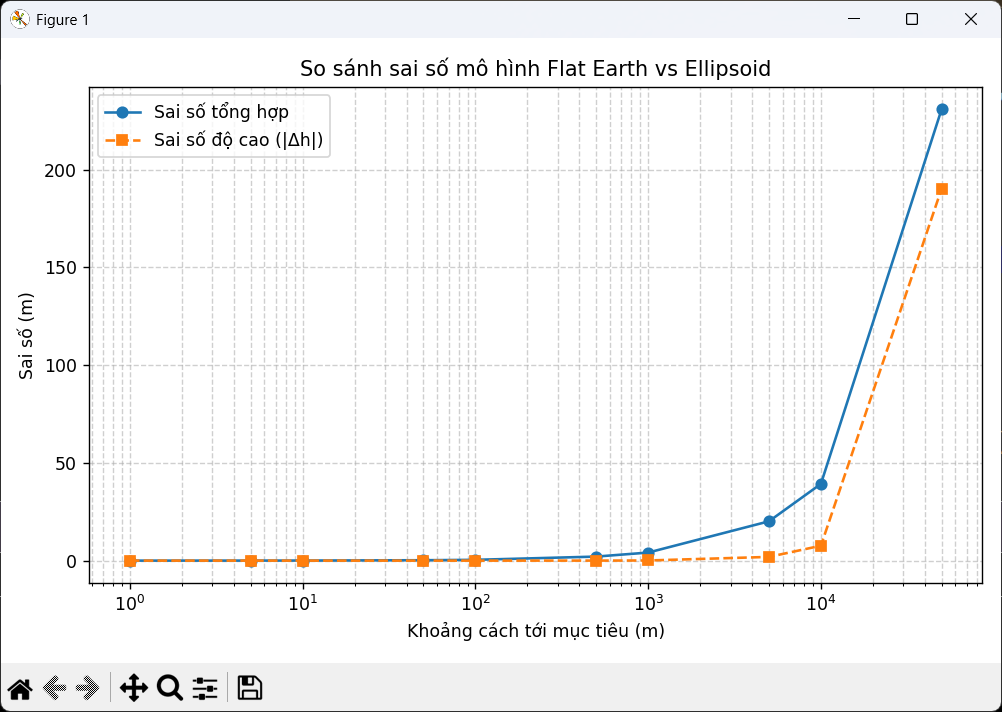
\includegraphics[scale=0.5]
    {Images/FlatEarth}
    \vspace{0.4cm} 
    \caption{Đồ thị biểu diễn kết quả so sánh sai số giữa 2 mô hình}
\end{figure}

\subsection{Kết luận}
\begin{itemize}
    \item Thuật toán \textbf{Flat-Earth (cải tiến)} đạt độ chính xác tương đương Geometric trong phạm vi vài km, đồng thời tính toán nhanh và đơn giản, phù hợp cho hệ thống nhúng hoặc UAV.
    \item Thuật toán \textbf{Geometric (ECEF$\rightarrow$ENU)} đảm bảo tính chính xác toàn cầu, thích hợp cho ứng dụng đo xa hoặc yêu cầu sai số ở mức cm.
\end{itemize}

\newpage
\section{Tổng kết và Hướng phát triển}

\subsection{Tổng kết Giai đoạn 1}
Trong Giai đoạn 1 của đồ án, nhóm đã tập trung nghiên cứu cơ sở lý thuyết và xây dựng nền tảng ban đầu cho hệ thống tính toán tọa độ mục tiêu. Các kết quả đạt được bao gồm:

\begin{itemize}
    \item \textbf{Nghiên cứu lý thuyết}:
    \begin{itemize}
        \item Tìm hiểu sâu về hệ thống định vị toàn cầu GPS, các hệ tọa độ không gian (Geodetic, ECEF, ENU, NED) và các phép chuyển đổi giữa chúng.
        \item Phân tích các nguồn sai số trong GPS và cảm biến (IMU, Laser Rangefinder) cũng như các phương pháp hiệu chuẩn cơ bản.
        \item Nắm vững nguyên lý tính toán trắc địa trên mặt cầu (Haversine) và mặt ellipsoid (Vincenty).
    \end{itemize}
    
    \item \textbf{Hiện thực ứng dụng (Prototype)}:
    \begin{itemize}
        \item Xây dựng thành công ứng dụng Web Map Viewer sử dụng thư viện Leaflet.js.
        \item Hiện thực module tính toán tọa độ mục tiêu từ vị trí quan sát, góc phương vị và khoảng cách với giao diện trực quan.
        \item Tích hợp các công cụ hỗ trợ như chuyển đổi định dạng tọa độ (DMS/Decimal), đo đạc khoảng cách và hiển thị trực quan trên bản đồ số.
    \end{itemize}
\end{itemize}

Hệ thống hiện tại hoạt động ổn định trên trình duyệt, đáp ứng tốt các yêu cầu cơ bản về tính toán và hiển thị trong phạm vi khoảng cách ngắn (< 100km) với sai số chấp nhận được cho các bài toán quan sát thông thường.

\subsection{Hạn chế}
Mặc dù đã đạt được những kết quả bước đầu, hệ thống vẫn còn một số hạn chế cần khắc phục:
\begin{itemize}
    \item \textbf{Mô hình toán học}: Vẫn sử dụng công thức Haversine trên mô hình cầu, chưa áp dụng triệt để mô hình Ellipsoid WGS-84 cho độ chính xác cao nhất ở khoảng cách xa.
    \item \textbf{Dữ liệu độ cao}: Chưa tích hợp dữ liệu độ cao (Elevation/DEM), dẫn đến việc tính toán chỉ dừng lại ở mặt phẳng 2D, bỏ qua sai số do chênh lệch độ cao giữa người quan sát và mục tiêu.
    \item \textbf{Lưu trữ}: Chưa có Backend và Cơ sở dữ liệu để lưu trữ lịch sử đo đạc, quản lý người dùng và chia sẻ dữ liệu giữa các nhóm.
\end{itemize}

\subsection{Hướng phát triển Giai đoạn 2}
Dựa trên kết quả và hạn chế của Giai đoạn 1, nhóm đề xuất kế hoạch phát triển cho Giai đoạn 2 như sau:

\begin{enumerate}
    \item \textbf{Nâng cấp thuật toán}:
    \begin{itemize}
        \item Chuyển đổi hoàn toàn sang công thức Vincenty hoặc Karney để tính toán trên Ellipsoid WGS-84.
        \item Tích hợp API lấy dữ liệu độ cao (Google Elevation API hoặc OpenTopography) để tính toán 3D (Slant range to Horizontal distance).
    \end{itemize}
    
    \item \textbf{Phát triển Backend}:
    \begin{itemize}
        \item Xây dựng Server (Node.js/Python) và Database (PostgreSQL/PostGIS) để quản lý dữ liệu không gian.
        \item Hiện thực API RESTful cho phép ứng dụng mobile hoặc thiết bị nhúng gửi dữ liệu trực tiếp.
    \end{itemize}
    
    \item \textbf{Tích hợp phần cứng (Hardware Integration)}:
    \begin{itemize}
        \item Kết nối thử nghiệm với module GPS (u-blox), IMU (MPU6050/9250) và Laser Rangefinder thực tế.
        \item Xây dựng luồng dữ liệu từ cảm biến $\rightarrow$ Vi điều khiển $\rightarrow$ Web Server.
    \end{itemize}
    
    \item \textbf{Nâng cao trải nghiệm người dùng}:
    \begin{itemize}
        \item Hỗ trợ bản đồ Offline (MBTiles).
        \item Thêm tính năng dẫn đường (Routing) đến mục tiêu đã xác định.
    \end{itemize}
\end{enumerate}
%%%%%%%%%%%%%%%%%OUTRO%%%%%%%%%%%%%%%%%%%
\renewcommand\refname{Tài liệu tham khảo}
\bibliographystyle{plain}
\bibliography{references}
\nocite{*} % Show all references even if not cited in text
% \newpage
% \input{Outro/PhuLuc}
\end{document}
